\documentclass[12pt,notitlepage]{article}

\usepackage{amsmath}
\usepackage{amssymb}
\usepackage{graphicx}
\usepackage{natbib}
\usepackage{tikz}
\usepackage{empheq}
\usepackage{cases}

\usepackage{titlesec}

\setcounter{secnumdepth}{4}

\titleformat{\paragraph}
{\normalfont\normalsize\bfseries}{\theparagraph}{1em}{}
\titlespacing*{\paragraph}
{0pt}{3.25ex plus 1ex minus .2ex}{1.5ex plus .2ex}

\usepackage{xcolor}
\usepackage{soul}
\definecolor{redhl}{rgb}{1,0.5,0.5}
\definecolor{bluehl}{rgb}{0.75,0.75,1}
\definecolor{greenhl}{rgb}{0.5,1.0,0.5}
\definecolor{tealhl}{rgb}{0.6,0.8,0.8}
\newcommand{\awnote}[1]{\sethlcolor{redhl}\hl{(AW: #1)}}
\newcommand{\dbnote}[1]{\sethlcolor{bluehl}\hl{(DB: #1)}}
\newcommand{\psnote}[1]{\sethlcolor{greenhl}\hl{(PS: #1)}}
\newcommand{\tknote}[1]{\sethlcolor{tealhl}\hl{(TK: #1)}}
\newcommand{\boxedeq}[2]{\begin{empheq}[box={\fboxsep=6pt\fbox}]{align}\label{#1}#2\end{empheq}}

% for atmosphere / volatiles
%\newcommand{\water}[0]{H$_2$O}
%\newcommand{\dih}[0]{H$_2$}

\newcommand{\myemph}[1]{\textbf{#1}}
\begin{document}

\title{Manual and extended notes for SPIDER\\[2ex] 
\includegraphics[width=0.5\textwidth]{figs/spider_logo}}
\author{Dan J. Bower}

\pagenumbering{Roman}

\maketitle

\tableofcontents
\newpage
\listoffigures
\newpage
\listoftables
\newpage
\pagenumbering{arabic}

%\begin{abstract}
%The abstract text goes here.
%\end{abstract}

%\section{Preface}
%This document is work in progress, and contains an extended description of the equations and derivations related to the SPIDER code \citep{BSW18}.  It essentially covers the physics and mathematics in more depth than is covered in \cite{ABE93,ABE95,BSW18}.  In fact, the notes in this document apply much more broadly than for just the SPIDER code, since they present the conservation equations for a multi-component system and are hence generally applicable to a range of fluid dynamical applications.  For example, this theory will also be applicable to recent melting and energy transport implementations in StagYY \citep{TACK08}.  There remains duplication of material in this document and several sections need to be reorganised.
%%%%
\subsection{Author contributions}
\begin{itemize}
\item \cite{BSW18} provided the base code
\item \cite{BKW19} added support for outgassing volatiles
\item Rob Spaargaren (ETHZ) added compositional dependent viscosity and discussion on the mixing length profile
\end{itemize}
%\clearpage

%\section{Fundamental thermodynamics}
%\label{sect:thermodynamic}
\fbox{\parbox{\textwidth}{Understand the origin of the energy transport associated with the enthalpy of chemical/phase components.  This derives the energy equation for a multi-component system that appears in the appendix of \cite{ABE95}.}}\\

\noindent
In the following section, I combine the notation from \cite{DM62} and \cite{ABE95} so beware of notation changes compared to the original papers.  Where a choice can be made, I typically stick to the notation of \cite{ABE95}.  Conservation of mass fraction \cite[Eq.~II.13,][]{DM62}, \cite[also Eq.~A2,][]{ABE95}, \myemph{where $i$ is a thermodynamic (chemical) component and $j$ refers to a reaction}:
\begin{equation}
\rho \frac{D \omega_i}{Dt} = -\nabla \cdot \vec{J}_i + \rho \sum_{j=1}^r \nu_{ij} \mathcal{J}_j \qquad (i=1,\ n)
\label{eq:ABE95_A2}
\end{equation}
Here I define \myemph{$\mathcal{J}_j$ as the rate of reaction $j$ per unit mass} (same as $w_j$ in \cite{ABE95} but this notation may be confused with mass fraction $\omega$ which is why I change the symbol).  \cite{ABE95} defines \myemph{$\nu_{ij}$ as the mass of component $i$ formed by reaction $j$}.  Note that \cite{DM62} use slightly different definitions of these quantities, since they define $\mathcal{J}$ as a mass per unit volume and unit time and omit the leading $\rho$ term.  Entropy balance \cite[Eq.~III.12,][]{DM62}, \cite[also Eq.~A4,][]{ABE95}:
\begin{equation}
\rho \frac{Ds}{Dt} = - \nabla \cdot \vec{J}_s + \sigma
\label{DM62_ch3_eq12}
\end{equation}
where the entropy flux $\vec{J}_s$ is the difference between the total entropy flux $\vec{J}_{s,\ tot}$ and a convective term $\rho s v$ \cite[Eq.~III.13,][]{DM62}:
\begin{equation}
\vec{J}_s = \vec{J}_{s,\ tot} - \rho s v
\end{equation}
The entropy balance, \myemph{excluding viscous dissipation and external forces}, is \cite[Eq.~III.19,][]{DM62}:
\begin{equation}
\rho \frac{Ds}{Dt} = - \nabla \cdot \left( \frac{\vec{J}_q - \sum_i \mu_i \vec{J}_i}{T} \right) - \frac{1}{T^2} \vec{J}_q \cdot \nabla T - \frac{1}{T} \sum_{i=1}^n \vec{J}_i \cdot T \nabla \left( \frac{\mu_i}{T} \right) - \frac{\rho}{T} \sum_{i=1}^n \sum_{j=1}^r \nu_{ij} \mu_i \mathcal{J}_j 
\end{equation}
Where entropy flux is \cite[Eq.~III.20,][]{DM62}:
\begin{equation}
\vec{J}_s = \frac{1}{T} \left( \vec{J}_q - \sum_{i=1}^n \mu_i \vec{J}_i \right)
\end{equation}
and entropy production is \cite[Eq.~III.21,][]{DM62}:
\begin{equation}
\sigma = - \frac{1}{T^2} \vec{J}_q \cdot \nabla T - \frac{1}{T} \sum_{i=1}^n \vec{J}_i \cdot T \nabla \left( \frac{\mu_i}{T} \right)
- \frac{\rho}{T} \sum_{i=1}^n \sum_{j=1}^r \nu_{ij} \mu_i \mathcal{J}_j
\end{equation}
By using the thermodynamic relation \cite[Eq.~III.23,][]{DM62}:
\begin{equation}
T d \left( \frac{\mu_i}{T} \right) = \left( d \mu_i \right)_T - \frac{h_i}{T} dT
\end{equation}
We can define a new flux as \cite[Eq.~III.24,][]{DM62}:
\begin{equation}
\vec{J}_q^\prime = \vec{J}_q - \sum_{i=1}^n h_i \vec{J}_i
\label{eq:Jqprime}
\end{equation}
\myemph{Eq.~\ref{eq:Jqprime} is the definition of heat flux used by \cite{ABE95} and therefore it removes the energetic contribution associated with the transport of enthalpy by the components.  This term then reappears as an entropy source term, since of course the physics must remain the same!}.
Then entropy flow is \cite[Eq.~III.26,][]{DM62}, \cite[also Eq.~A5,][]{ABE95}:
\begin{equation}
\vec{J}_s = \frac{1}{T} \vec{J}_q^\prime + \sum_{i=1}^n s_i \vec{J}_i
\label{DM62_ch3_eq26}
\end{equation}
where $s_i = -(\mu_i-h_i)/T$ is the partial specific entropy of component $i$.  \myemph{Written in this way the entropy flux contains the heat flow $\vec{J}_q^\prime$ and a transport of partial entropies with respect to the barycentric velocity $v$}.  The entropy production associated with this definition can be written as \cite[Eq.~III.25,][]{DM62}, \cite[also Eq.~A6,][]{ABE95}:
\begin{equation}
\sigma = - \frac{1}{T^2} \vec{J}_q^\prime \cdot \nabla T - \frac{1}{T} \sum_{i=1}^n \vec{J}_i \cdot \left( \nabla \mu_i \right)_T - \frac{\rho}{T} \sum_{i=1}^n \sum_{j=1}^r \nu_{ij} \mu_i \mathcal{J}_j
\label{eq:DM62_ch3_eq25}
\end{equation}
%%%
Quoting from \cite{DM62}:\\

\emph{``It is clear that the difference between $\vec{J}_q$ and $\vec{J}_q^\prime$ (Eq.~\ref{eq:Jqprime}) represents a transfer of heat due to diffusion. Therefore the quantity $\vec{J}_q^\prime$ also represents an irreversible heat flow. In fact in diffusing mixtures the concept of heat flow can be defined in different ways. Obviously a different definition of the notion of heat flux leaves all physical results unchanged. But to any particular choice corresponds a special form of the entropy production $\sigma$. It is a matter of expediency which choice is the most suitable in a particular application of the theory. The freedom of defining the heat flow in various ways, of which the possibility was indicated here in the framework of a macroscopic treatment, exists also in the microscopic theories of transport phenomena in mixtures.''}\\

Abe chooses to model $J_q^\prime$ as a convective heat flux using mixing length theory.  In this regard, \cite[Eq.~47,][]{ABE95} \myemph{excludes the energetic contribution of the enthalpy transport of the components (but remember it appears later in Abe's formulation)}.  Now, using the above equations we can derive \cite[Eq.~A10,][]{ABE95} using several vector identities:
%%%
\begin{align}
\rho \frac{Ds}{Dt} &= -\nabla \cdot \left(  \frac{1}{T} \vec{J}_q^\prime + \sum_{i=1}^n s_i \vec{J_i} \right) + \sigma \\
&= - \frac{1}{T} \nabla \cdot \vec{J}_q^\prime + \frac{1}{T^2} \vec{J}_q^\prime \cdot \nabla T - \sum_{i=1}^n \nabla s_i \cdot \vec{J}_i - \sum_{i=1}^n s_i \nabla \cdot \vec{J}_i + \sigma
\end{align}
Sub in $\sigma$ (Eq.~\ref{eq:DM62_ch3_eq25}) and immediately see that the $1/T^2$ term cancels leaving:
\begin{equation}
\rho \frac{Ds}{Dt} = - \frac{1}{T} \nabla \cdot \vec{J}_q^\prime - \sum_{i=1}^n \nabla s_i \cdot \vec{J}_i - \sum_{i=1}^n s_i \nabla \cdot \vec{J}_i - \frac{1}{T} \sum_{i=1}^n \vec{J}_i \cdot (\nabla \mu_i)_T - \frac{\rho}{T} \sum_{i=1}^n \sum_{j=1}^r \nu_{ij} \mu_i \mathcal{J}_j
\end{equation}
Now use Eq.~\ref{eq:ABE95_A2} to eliminate the chemical reaction term:
\begin{equation}
\rho \frac{Ds}{Dt} = - \frac{1}{T} \nabla \cdot \vec{J}_q^\prime - \sum_{i=1}^n \nabla s_i \cdot \vec{J}_i - \sum_{i=1}^n s_i \nabla \cdot \vec{J}_i - \frac{1}{T} \sum_{i=1}^n \vec{J}_i \cdot (\nabla \mu_i)_T - \frac{1}{T} \sum_{i=1}^n \left( \mu_i \rho \frac{D\omega_i}{Dt} +\mu_i \nabla \cdot \vec{J}_i \right)
\end{equation}
Collect terms.  \myemph{\cite{ABE95} missing $\rho$ on the RHS}:
\begin{equation}
\rho \frac{Ds}{Dt} = - \frac{1}{T} \nabla \cdot \vec{J}_q^\prime - \sum_{i=1}^n \nabla \cdot (s_i \vec{J}_i ) - \frac{1}{T} \sum_{i=1}^n \nabla \cdot (\mu_i \vec{J}_i) - \frac{\rho}{T} \sum_{i=1}^n \mu_i  \frac{D\omega_i}{Dt}
\end{equation}
Now use $h_i = \mu_i + T s_i$:
\begin{equation}
\rho \frac{Ds}{Dt} = - \frac{1}{T} \nabla \cdot \vec{J}_q^\prime - \frac{1}{T} \sum_{i=1}^n \nabla \cdot (h_i \vec{J}_i ) - \frac{\rho}{T} \sum_{i=1}^n \mu_i  \frac{D\omega_i}{Dt}
\end{equation}
Leading to \cite[Eq.~A10,][]{ABE95}, \myemph{\cite[Eq.~A10,][]{ABE95} missing $\rho$}:
\boxedeq{}{\rho \frac{Ds}{Dt} = - \frac{1}{T} \nabla \cdot \left( \vec{J}_q^\prime + \sum_{i=1}^n h_i \vec{J}_i \right) - \frac{\rho}{T} \sum_{i=1}^n \mu_i  \frac{D\omega_i}{Dt}}
How \cite[Eq.~4][]{ABE95} is derived from this point is confusing.  It appears that if you literally swap out components and replace them with phases, where the two phases are melt and solid, you can reproduce \cite[Eq.~4][]{ABE95}.  But then later, \cite{ABE95} states that this equation must be \emph{``modified for multi-component systems, because energy transport due to mass transport must be taken into account''}.  He then goes onto to derive the following equation, which makes sense based on \cite[Eq.~A10,][]{ABE95}.  The transport of thermodynamic components can be divided between a melt and solid phase.  \myemph{This is how the notion of phases is introduced into the formulation}.
\begin{equation}
\sum_{i=1}^n h_i\vec{J}_i = \sum_{i=1}^n h_i^m \vec{J}_i^m + h_i^s \vec{J}_i^s
\end{equation}
where $h_i^m$ and $h_i^s$ are the partial specific enthalpy of component $i$ in melt and solid phases, respectively.  Now recognise that the following holds, since the we can split the flux into a part relative to the velocity of the melt:
\begin{subequations}
\begin{align}
\vec{J}_i^m&= \rho \phi \omega_i^m (\vec{U}_i^m - \vec{U} )\\
&= \rho \phi \omega_i^m (\vec{U}_i^m - \vec{U}_{m} + \vec{U}_m - \vec{U} )\\
&= \rho \phi \omega_i^m (\vec{U}_i^m - \vec{U}_{m} ) + \rho \phi \omega_i^m ( \vec{U}_m - \vec{U} )\\
&= \vec{j}_i^m + \omega_i^m \vec{J}_m
\end{align}
\label{eq:J_mi}
\end{subequations}
and similarly:
%%%
\begin{subequations}
\begin{align}
\vec{J}_i^s&= \rho (1-\phi) \omega_i^s (\vec{U}_i^s - \vec{U} )\\
&= \rho (1-\phi) \omega_i^s (\vec{U}_i^s - \vec{U}_s + \vec{U}_s - \vec{U} )\\
&= \rho (1-\phi) \omega_i^s (\vec{U}_i^s - \vec{U}_s) + \rho (1-\phi) \omega_i^s (\vec{U}_{s} - \vec{U})\\
&= \vec{j}_i^s + \omega_i^s \vec{J}_s\\
&= \vec{j}_i^s - \omega_i^s \vec{J}_m
\end{align}
\label{eq:J_si}
\end{subequations}
where $\omega_i^m$, $\omega_i^s$, $\vec{J}_i^m$, and $\vec{J}_i^s$ are the mass fraction and mass flux of component $i$ in melt and solid phases, respectively.  $j_i^m$ and $j_i^s$ are the mass fluxes of component $i$ in melt and solid phases, respectively, caused by mechanisms other than melt-solid relative motion.  Substitute in Eqs.~\ref{eq:J_mi} and \ref{eq:J_si}:
\begin{equation}
\sum_{i=1}^n h_i\vec{J}_i = \sum_{i=1}^n h_i^m \vec{J}_i^m + h_i^s \vec{J}_i^s =  \sum_{i=1}^n h_i^m \left( \vec{j}_i^m + \omega_i^m \vec{J}_m \right) + h_i^s \left( \vec{j}_i^s - \omega_i^s \vec{J}_m \right)
\end{equation}
and collect terms:
\begin{align}
\sum_{i=1}^n h_i\vec{J}_i &= \vec{J}_m \sum_{i=1}^n \left( h_i^m \omega_i^m - h_i^s \omega_i^s \right) + \sum_{i=1}^n h_i^m \vec{j}_i^m + h_i^s \vec{j}_i^s\\
&= \vec{J}_m \left( h^m - h^s \right) + \sum_{i=1}^n h_i^m \vec{j}_i^m + h_i^s \vec{j}_i^s\\
&= \Delta h \vec{J}_m + \sum_{i=1}^n h_i^m \vec{j}_i^m + h_i^s \vec{j}_i^s
\end{align}
This is helpful because the gravitational separation term (first term) can be parameterised simply based on Stokes' law.  The second term within the summation ultimately becomes the ``mixing term'' (see below), which represents energy transport due to mechanisms other than relative melt--solid separation.

For two phases ($n=2$) and $J_m=-J_s$, \myemph{\cite[Eq.~4,][]{ABE95} missing $\rho$}:
\boxedeq{eq:entropy_twophase}{\rho \frac{Ds}{Dt} = - \frac{1}{T} \nabla \cdot \left( \vec{J}_q^\prime + (h_m-h_s) \vec{J}_m \right) - \frac{\rho}{T} (\mu_m-\mu_s) \frac{D\phi}{Dt}}
Note this contains a latent heat ($\Delta h$) associated with melt--solid separation ($\vec{J}_m$).  At chemical equilibrium, which we always assume, $\mu_m=\mu_s$ and hence the last term is zero.  Now, for multi-component systems, energy transport due to mass transport must be taken into account \myemph{\cite[Eq.~20,][]{ABE95} missing $\rho$}:
\begin{align}
\begin{split}
\rho \frac{Ds}{Dt} &= -\frac{1}{T} \nabla \cdot \left[ \vec{J}_q^\prime + \Delta h \vec{J}_m + \sum_{i=1}^n (h_{mi} \vec{j}_{mi} + h_{si} \vec{j}_{si} ) \right]\\
&\qquad -\frac{\rho}{T} \left[ \Delta \mu \frac{D\phi}{Dt} + \sum_{i=1}^n \left( \phi \mu_{mi}\frac{D\omega_{mi}}{Dt} + (1-\phi) \mu_{si} \frac{D\omega_{si}}{Dt} \right) \right]
\end{split}
\end{align}
Under the assumption of chemical equilibrium, the final term of Eq.~\ref{eq:entropy_twophase} is zero.  We then arrive at the fundamental equation that we solve in the SPIDER code.
\boxedeq{eq:entropy_twophase_chemeq}{\rho \frac{Ds}{Dt} = - \frac{1}{T} \nabla \cdot \left( \vec{J}_q^\prime + (h_m-h_s) \vec{J}_m \right)}
With temperature as the primary variable \myemph{\cite[Eq.~10,][]{ABE95}}:
\boxedeq{eq:temperature_twophase_chemeq}{\rho C_p \frac{DT}{Dt} = - \nabla \cdot \left( \vec{J}_q^\prime + (h_m-h_s) \vec{J}_m \right) - \rho (h_m-h_s) \frac{D\phi}{Dt}}

\noindent The two major steps that we now need to perform are:
\begin{enumerate}
\item Recast the velocities in terms of relative velocities, often relative to the centre of mass (barycentric velocity).
\item Parameterise the resulting fluxes that originate from considering relative velocities.
\end{enumerate}

%\clearpage

%\section{Conservation of chemical species}
%
\subsection{Conservation of mass}

\fbox{\parbox{\textwidth}{Eulerian and Lagrangian forms of mass conservation.}}\\

\noindent
Eulerian:
\begin{equation}
\frac{\partial \rho}{\partial t} + \nabla \cdot ( \rho \vec{U} ) = 0
\end{equation}
Lagrangian (e.g., A1 in \cite{ABE95}):
\begin{equation}
\frac{D \rho}{Dt} + \rho \nabla \cdot \vec{U} = 0
\end{equation}
Material derivative:
\begin{equation}
\frac{D}{Dt} \equiv \frac{\partial}{\partial t} + \vec{U} \cdot \nabla
\end{equation}
where $\rho$ is density, $U$ velocity, $t$ time.  There are no sources or sinks of mass for global mass conservation.

\subsection{Barycentric velocity}

\fbox{\parbox{\textwidth}{Description of the barycentric velocity and measuring the velocity of chemical species relative to it.}}\\

\noindent
The total number of moles in a unit volume $n_t$, is obtained by summing over all the contributions of the \textbf{number of moles per unit volume} of each species, $n_i$:
\begin{equation}
n_t = \sum_i n_i
\end{equation}
The density of the fluid is given by summation over the partial densities of all the species:
\begin{equation}
\rho = \sum_i \rho_i
\end{equation}
where:
\begin{equation}
\rho_i = n_i \mathcal{M}_i
\end{equation}
where $\mathcal{M}_i$ is the molecular weight of species $i$.  The molecular weight of the mixture is:
\begin{equation}
\overline{\mathcal{M}} = \sum_i x_i \mathcal{M}_i
\end{equation}
where $x_i=n_i/n_t$ is mole fraction of species $i$.  So the density of the mixture is:
\begin{equation}
\rho = n_t \overline{\mathcal{M}}
\end{equation}
The mass fraction of species $i$, $\omega_i$:
\begin{equation}
\omega_i = \frac{\rho_i}{\rho} = \frac{n_i \mathcal{M}_i}{\rho}
\label{eq:rhoi}
\end{equation}
The absolute molar flux of species $i$ with respect to \textbf{fixed spatial coordinate} is given by:
\begin{equation}
n_i \vec{U}_i
\end{equation}
hence the mass flux of species $i$ with respect to \textbf{fixed spatial coordinate} is given by:
\begin{equation}
\vec{J}^\ast_i = n_i \mathcal{M}_i \vec{U}_i = \rho \omega_i \vec{U}_i = \rho_i \vec{U}_i
\label{eq:Jast}
\end{equation}
The mass-weighted average velocity of the fluid $\vec{U}$ (also know as the stream velocity or \textbf{barycentric velocity}) is:
\begin{equation}
\rho \vec{U} = \sum_i \vec{J}^\ast_i = \sum_i \rho_i \vec{U}_i
\end{equation}
\begin{equation}
\vec{U} = \frac{1}{\rho} \sum_i \rho_i \vec{U}_i = \frac{1}{\rho} \sum_i n_i \mathcal{M}_i \vec{U}_i = \sum_i \omega_i \vec{U}_i
\label{eq:barycentric}
\end{equation}
The velocity of species $i$ \textbf{relative to the barycentric velocity} (sometimes called the diffusion or streaming velocity) is:
\begin{equation}
\vec{u}_i = \vec{U}_i - \vec{U}
\label{eq:diffusionvelocity}
\end{equation}
We can now define the \textbf{relative or diffusion flux vector}:
\begin{equation}
\vec{J}_i = \rho_i ( \vec{U}_i - \vec{U}) = \rho_i \vec{u}_i
\label{eq:diffusionflux}
\end{equation}
Note that the mass-weighted average of the diffusion velocity is zero as follows:
\begin{align}
\frac{1}{\rho} \sum_i \rho_i \vec{u}_i &= \frac{1}{\rho} \sum_i \rho_i \vec{U}_i - \frac{1}{\rho} \sum_i \rho_i \vec{U}\\
&= \frac{1}{\rho} (\rho \vec{U}) - \frac{\vec{U}}{\rho} (\rho) = 0
\end{align}
Consequently we can write:
\begin{equation}
\sum_i \vec{J}_i = \sum_i \rho_i \vec{u}_i = 0
\end{equation}
%%%%%%%%%%%
%%% Eulerian %%%
%%%%%%%%%%%
\subsection{Eulerian description with barycentric velocity}
\fbox{\parbox{\textwidth}{Eulerian description for the conservation of mass fraction of species $i$ in terms of the barycentric velocity and fluxes relative to the barycentric velocity.}}\\

\noindent
Conservation of species $i$ in terms of moles per unit volume:
\begin{equation}
\frac{\partial n_i}{\partial t} + \nabla \cdot n_i \vec{U}_i = \dot{M}_i
\end{equation}
where $\dot{M}_i$ is net molar production of species $i$ per unit volume by chemical reaction.  Equivalently:
\begin{equation}
\frac{\partial \rho_i}{\partial t} + \nabla \cdot \vec{J}^\ast_i = \rho \dot{w}_i
\end{equation}
where the chemical source function $\dot{w}$ represents the mass rate of production of species $i$ by chemical reaction \textbf{per unit mass} and may be determined from chemical kinetics.  \textbf{$\vec{J}^\ast_i$ is relative to a fixed reference frame}.  Substitute in expression for $\vec{J}^\ast_i$ using Eqs.~\ref{eq:Jast} and \ref{eq:diffusionvelocity} to eliminate $\vec{U}_i$:
\begin{equation}
\frac{\partial \rho_i}{\partial t} + \nabla \cdot \rho_i (\vec{U} + \vec{u}_i)= \rho \dot{w}_i
\end{equation}
Expand $\nabla$ and substitute in $\rho_i= \rho \omega_i$ (Eq.~\ref{eq:rhoi}):
\begin{equation}
\frac{\partial (\rho \omega_i)}{\partial t}  + \nabla \cdot \rho \omega_i \vec{U} + \nabla \cdot \rho_i \vec{u}_i = \rho \dot{w}_i
\end{equation}
Substitute in $\vec{J}_i$ (Eq.~\ref{eq:diffusionflux}) (\textbf{recall this is relative to the barycentre}):
\begin{align}
\frac{\partial (\rho \omega_i)}{\partial t} + \nabla \cdot \rho \omega_i \vec{U} &= - \nabla \cdot \vec{J}_i + \rho \dot{w}_i\\
\rho \frac{\partial \omega_i}{\partial t} + \omega_i \frac{\partial \rho}{\partial t} + \rho \omega_i \nabla \cdot \vec{U} + \vec{U} \cdot \nabla (\rho \omega_i) &= - \nabla \cdot \vec{J}_i + \rho \dot{w}_i \label{eq:eulerianworking}
\end{align}
Global mass conservation (no sources or sinks of mass):
\begin{equation}
\frac{\partial \rho}{\partial t} = - \nabla \cdot (\rho \vec{U} ) = -\rho \nabla \cdot \vec{U} - \vec{U} \cdot \nabla \rho
\end{equation}
Substitute in Eq.~\ref{eq:eulerianworking}:
\begin{equation}
\rho \frac{\partial \omega_i}{\partial t} - \omega_i \vec{U} \cdot \nabla \rho + \vec{U} \cdot \nabla (\rho \omega_i) = - \nabla \cdot \vec{J}_i + \rho \dot{w}_i
\end{equation}
Expand remaining $\nabla$:
\begin{equation}
\vec{U} \cdot \nabla(\rho \omega_i) = \omega_i \vec{U} \cdot \nabla \rho + \rho \vec{U} \cdot \nabla \omega_i
\label{eq:eulerianworking2}
\end{equation}
Substitute in Eq.~\ref{eq:eulerianworking2}:
\begin{equation}
\rho \frac{\partial \omega_i}{\partial t} + \rho \vec{U} \cdot \nabla \omega_i = - \nabla \cdot \vec{J}_i + \rho \dot{w}_i
\end{equation}
\boxedeq{eq:eulerianfinal}{\frac{\partial \omega_i}{\partial t} + \vec{U} \cdot \nabla \omega_i = -\frac{1}{\rho} \nabla \cdot \vec{J}_i + \dot{w}_i}
%%%%%%%%%%%%
%%% Lagrangian %%%
%%%%%%%%%%%%
\subsection{Lagrangian description with barycentric velocity}
\fbox{\parbox{\textwidth}{Lagrangian description for the conservation of mass fraction of species $i$ in terms of the barycentric velocity and fluxes relative to the barycentric velocity.}}\\

\noindent
Use the material derivative, where $U$ is the centre of mass velocity or equivalently the velocity of fluid element moving with the local barycentre:
\begin{equation}
\frac{D}{D t} \equiv \frac{\partial}{\partial t} + \vec{U} \cdot \nabla
\end{equation}
Substitute in Eq.~\ref{eq:eulerianfinal} (agrees with Eq.~A2 in \cite{ABE95}):
\boxedeq{eq:lagrangianfinal}{\rho \frac{D \omega_i}{Dt} = -\nabla \cdot \vec{J}_i + \rho \dot{w}_i}
%%%%
%%%%
%%%%
\subsection{Melt transport with barycentric velocity}
\fbox{\parbox{\textwidth}{Lagrangian description for the conservation of melt fraction and expressions for the mass flux of melt and solid relative to the barycentric velocity.}}\\

\noindent
Analogous to chemical species transport (Eq.~\ref{eq:lagrangianfinal}), we can consider the evolution of melt fraction $\phi$ (Eq.~2 in \cite{ABE95}):
\boxedeq{}{\rho \frac{D \phi}{D t} = - \nabla \cdot \vec{J}_m + \rho M}
where $\phi$ is melt fraction, $\vec{J}_m$ is the mass flux of melt with \textbf{respect to local barycentric motion} (the motion of the local barycentre of a fluid element composed of melt-solid mixture), and $M$ the melting rate per unit mass.  When we consider an $n$-component system, only $n-1$ equations are independent because the sum of mass fraction is unity.  Therefore, for the simple case of a melt--solid mixture (2 components) we only need one equation for melt fraction.  \myemph{SPIDER actually determines the melt fraction directly from a lookup table using the current pressure and entropy and the predefined melting curves, rather than explicitly tracking its evolution.} For a mixture of melt and solid, the \textbf{barycentric velocity} $U$ (Eq.~\ref{eq:barycentric}) is:
\begin{equation}
\vec{U} = \phi \vec{U}_m + (1-\phi) \vec{U}_s
\label{eq:U_barycentre}
\end{equation}
where $U_m$ and $U_s$ are the velocity of the melt and solid phase, respectively.  Now consider fluxes:
\begin{align}
\vec{J}_m &= \rho \phi (\vec{U}_m - \vec{U}) = -\vec{J}_s \label{eq:Jm}\\
\vec{J}_s &= \rho (1-\phi) (\vec{U}_s - \vec{U}) = -\vec{J}_m \label{eq:Js}
\end{align}
where $\vec{J}_m$ and $\vec{J}_s$ are the mass flux of melt and solid, respectively, \textbf{relative to the barycentre}.  Since the mass flux of melt or solid is caused by the differential motion of the solid and the melt phases, the mass flux is given as a function of relative velocity between the solid and the melt phases and melt fraction.  Eliminating $U$ in Eq.~\ref{eq:Jm} using Eq.~\ref{eq:U_barycentre}:
\begin{equation}
\vec{J}_m=-\vec{J}_s=\rho \phi (1-\phi) (\vec{U}_m-\vec{U}_s)
\end{equation}
\subsection{Melt and chemical species transport}
\fbox{\parbox{\textwidth}{Lagrangian description for the conservation of chemical species assuming partitioning between melt and solid phase at thermodynamic equilibrium.}}\\

\noindent
Following \cite{ABE95}, we now introduce $i$ components, which are chemical species that we wish to track, and each component can exist in the melt or the solid phase.  We have two equations that describe the mass fraction of each component in the melt or solid phase:

\begin{equation}
\rho \frac{D}{Dt} (\phi \omega_{mi} ) = -\nabla \cdot \vec{J}_{mi} + \rho M_i \qquad (i=1,n)
\label{eq:cons_omega_mi}
\end{equation}

\begin{equation}
\rho \frac{D}{Dt} ((1-\phi) \omega_{si} ) = -\nabla \cdot \vec{J}_{si} - \rho M_i \qquad (i=1,n)
\label{eq:cons_omega_si}
\end{equation}
where $\omega_{mi}$, $\omega_{si}$, $\vec{J}_{mi}$, and $\vec{J}_{si}$ are the mass fraction and mass flux of component $i$ in melt and solid phases, respectively, and $M_i$ is the mass melting rate of chemical component $i$ per unit mass.  From the definition of mass flux relative to the barycentre (e.g., analogous to Eqs.~\ref{eq:Jm} and \ref{eq:Js}), $\vec{J}_{mi}$ and $\vec{J}_{si}$ are:
%%%
\begin{subequations}
\begin{align}
\vec{J}_{mi}&= \rho \phi \omega_{mi} (\vec{U}_{mi} - \vec{U} )\\
&= \rho \phi \omega_{mi} (\vec{U}_{mi} - \vec{U}_{m} + \vec{U}_m - \vec{U} )\\
&= \rho \phi \omega_{mi} (\vec{U}_{mi} - \vec{U}_{m} ) + \rho \phi \omega_{mi} ( \vec{U}_m - \vec{U} )\\
&= \vec{j}_{mi} + \omega_{mi} \vec{J}_m
\end{align}
\label{eq:J_mi2}
\end{subequations}
%%%
\begin{subequations}
\begin{align}
\vec{J}_{si}&= \rho (1-\phi) \omega_{si} (\vec{U}_{si} - \vec{U} )\\
&= \rho (1-\phi) \omega_{si} (\vec{U}_{si} - \vec{U}_s + \vec{U}_s - \vec{U} )\\
&= \rho (1-\phi) \omega_{si} (\vec{U}_{si} - \vec{U}_s) + \rho (1-\phi) \omega_{si} (\vec{U}_{s} - \vec{U})\\
&= \vec{j}_{si} + \omega_{si} \vec{J}_s\\
&= \vec{j}_{si} - \omega_{si} \vec{J}_m
\end{align}
\label{eq:J_si2}
\end{subequations}
where:
\begin{equation}
\vec{j}_{mi} \equiv \rho \phi \omega_{mi} ( \vec{U}_{mi}-\vec{U}_m ), \qquad \vec{j}_{si} \equiv \rho (1-\phi) \omega_{mi} (\vec{U}_{si}-\vec{U}_s)
\end{equation}
$\vec{j}_{mi}$ and $\vec{j}_{si}$ are the mass fluxes of component $i$ in melt and solid phases, respectively, \textbf{caused by mechanisms other than melt--solid relative motion}.  Now add Eq.~\ref{eq:cons_omega_mi} and Eq.~\ref{eq:cons_omega_si}, and using Eq.~\ref{eq:J_mi} and Eq.~\ref{eq:J_si} and additionally introducing the mass fraction of component $i$ in the mixture, $\omega_i$ gives:
\begin{equation}
\rho \frac{D\omega_i}{Dt} = -\nabla \cdot \left[ (\omega_{mi}-\omega_{si}) \vec{J}_m + \vec{j}_{mi} + \vec{j}_{si} \right]
\label{eq:Domegai}
\end{equation}
\begin{equation}
\omega_i \equiv \phi \omega_{mi} + (1-\phi) \omega_{si} \qquad (i=1,\ n)
\end{equation}
Sum of mass fractions is unity, so only $n-1$ equations are independent.  Next, consider the case in which solid and melt phases are in chemical equilibrium:
\begin{equation}
\left( \frac{\omega_{si}}{\omega_{mi}} \right)_{at\ equilibrium} = K_{ei}
\end{equation}
Can now rewrite Eq.~\ref{eq:Domegai} using $K_{ei}$:
\begin{equation}
\rho \frac{D \omega_i}{D t} = - \nabla \cdot \left[ \frac{1-K_{ei}}{\phi_e+(1-\phi_e)K_{ei}} \omega_i \vec{J}_{m} + \vec{j}_{mi} + \vec{j}_{si} \right]
\label{eq:Domegai2}
\end{equation}
where $\phi_e$ is the melt fraction at the equilibrium.  We can approximate the convective mass transport by turbulent diffusion in a vigorously convecting layer.  Then vertical mass flux of component $i$ due to convection is given by Fick's law:
\begin{equation}
\vec{j}_{mi} = -\kappa_c \rho \frac{\partial \phi \omega_{mi}}{\partial r}, \qquad \vec{j}_{si} = -\kappa_c \rho \frac{\partial (1-\phi) \omega_{si}}{\partial r}
\end{equation}
where $\omega_{mi}$, $\omega_{si}$ and $\kappa_c$ are the mass fraction of component $i$ within melt and solid phases, and the eddy diffusivity for convective mass transport, respectively.  Then the net convective transport is:
\begin{equation}
\vec{j}_{mi} + \vec{j}_{si} = -\kappa_c \rho \frac{\partial \omega_i}{\partial r}
\end{equation}
So now we can express Eq.~\ref{eq:Domegai2} as:
\boxedeq{}{\rho \frac{D \omega_i}{D t} = - \nabla \cdot \left[ \frac{1-K_{ei}}{\phi_e+(1-\phi_e)K_{ei}} \omega_i \vec{J}_{m} - \rho \kappa_c \frac{\partial \omega_i}{\partial r} \right]}
On the RHS the first term is due to melt--solid relative motion and the second term is due to other mechanisms.

\subsection{Energy transport}
\fbox{\parbox{\textwidth}{Energy conservation in terms of entropy.}}\\

\noindent
Eq. 27 in \cite{ABE95}:
\begin{equation}
\rho T \frac{Ds}{Dt} = -\nabla \cdot \left[ \vec{J}_q + \Delta h \vec{J}_m + \sum_{i=1}^n (h_{mi} \vec{j}_{mi} + h_{si}\vec{j}_{si}) \right]
\end{equation}
Analyse the last term on the RHS:
\begin{align}
\sum_{i=1}^n (h_{mi} \vec{j}_{mi} + h_{si}\vec{j}_{si}) &= -\kappa_c \rho \sum_{i=1}^n \left(h_{mi} \frac{\partial \phi \omega_{mi}}{\partial r} + h_{si} \frac{\partial (1-\phi) \omega_{si}}{\partial r} \right)\\
&= -\kappa_c \rho \sum_{i=1}^n \left[ (h_{mi} \omega_{mi} - h_{si} \omega_{si})\frac{\partial \phi}{\partial r} + h_{mi} \phi \frac{\partial \omega_{mi}}{\partial r} + h_{si} (1-\phi) \frac{\partial \omega_{si}}{\partial r} \right]\\
&= -\kappa_c \rho \sum_{i=1}^n \left[ (h_{mi} \omega_{mi} - h_{si} \omega_{si})\frac{\partial \phi}{\partial r} \right]\\
&= -\kappa_c \rho \Delta h \frac{\partial \phi}{\partial r} \equiv \Delta h \vec{J}_{cm}
\end{align}

\textbf{The convective (phase) mixing term can probably be incorporated into the heat flux(?) if we modify the form of $\kappa_h$.  Or maybe if we decompose the velocities relative to the barycentre differently.  So rather than considering a term associated with melt--solid separation and another, we wrap them both up in the same formulation.  But combining with the convective heat flux seems to make the most sense since these are two terms, opposite in sign for $dS_{liq}/dr<0$ that nearly cancel.  The precision issue arises because this cancellation goes away for $dS_{liq}/dr>0$ and hence $dS/dr$ is driven to a tiny value.}
\boxedeq{}{\rho T \frac{Ds}{Dt} = -\nabla \cdot \left[ \vec{J}_q + \Delta h (\vec{J}_m + \vec{J}_{cm}) \right]}

%\clearpage

%\section{Material properties}
%\subsection{Mantle EOS}
A simple approximation is made to calculate the thermodynamic properties of the mantle silicates, representing them as a pseudo-single-component system.
We consider a mantle that is everywhere in local thermodynamic equilibrium, resulting in uniform compositional profiles.  Driven by buoyancy differences, crystals that form are displaced from their point of crystallization, instantaneously removing heat as they are resorbed by the magma ocean (according to Clausius Clapeyron).  Crystal-melt separation should cause chemical differentiation, however if the timescales for turbulent mixing are sufficiently fast, the mantle will remain homogenous.  Furthermore, persistent differentiation (which is expected for the later stages of crystallization as viscosity rises and timescales lengthen) represents a second-order correction on top of the first order energetics represented by convection, heat dissipation, and crystallization of a uniform composition magma ocean.

We represent the thermodynamics of mantle melting using a pseudo-one-component model, which retains the simplicity of a standard one-component model, while introducing the important multi-component characteristic of a finite temperature interval for melting.  We develop this model in response to the arguments of \cite{SA07}, which shows how many of the most important aspects of mantle melting can be reasonably-represented by a simple one-component model when viewed in pressure-entropy space.  Besides its lack of chemical evolution, the primary shortcoming of this approach is the absence of a thermal melting interval, which arises due to differential chemical partitioning between solid and melt phases, as demonstrated by simple systems with binary loops.  It is a useful first approximation to consider a crystallizing magma ocean as a chemically homogenous system, where the evolving chemistries of its constituent phases are assumed to remain in thermodynamic equilibrium maintaining constant bulk composition.  We can therefore approximate the energetics of this system by modifying a standard one-component system, replacing the univariant melting curve in P-T space $T_{\rm fus}(P)$ by a melting interval.
The single-component melting curve is given by $T_{\rm fus}(P)$ and $S_{\rm fus}(P)$, and is defined by the condition of equilibrium, where the solid and melt phases have equal Gibbs energies at the melting temperature for each pressure.
The modified melting interval is centered on the fusion curve, bounded by the liquidus above and solidus below:
\begin{eqnarray}
T_{\rm liq}(P) = T_{\rm fus}(P) + \Delta T_{\rm fus}(P) \big/ 2\\
T_{\rm sol}(P) = T_{\rm fus}(P) - \Delta T_{\rm fus}(P) \big/ 2
\end{eqnarray}
where the melting interval width is defined by \mbox{$\Delta T_{\rm fus}(P)=\delta T \cdot T_{\rm fus}(P)$} with $\delta T \approx 0.07$ throughout the mantle \citep{SKS09}.
%%%%
\subsection{Solid EOS}
For the Mosenfelder MgSiO3 model, we use the EOS for MgSiO3 melt and Mg-endmember bridgmanite as given by the global fit to shock wave and diamond anvil cell data in \cite{M09}.  Since this paper does not fully define all of the needed EOS parameters, we rely upon the estimated melting region (bounded by solidus and liquidus profiles) for the mantle given by \cite{SKS09}.  It is important to recognize that \cite{M09} does not present a thermodynamically consistent model of this system, due to its  use of the Mie-Gr\"{u}neisen formulation, which assumes that the gr\"{u}neisen parameter is independent of temperature together with its model for the heat capacity of the melt, which induces temperature dependence to the adiabatic compression curves.

The primary thermodynamic property controlling magma ocean evolution is the gr\"{u}neisen parameter, $\gamma$, which controls the adiabatic thermal profile through a convecting system:
\begin{equation}
\frac{dT}{dP}\bigg|_S = \gamma \left( \frac{T}{K_S} \right)
\label{eq:adiabatprof}
\end{equation}
The {\it thermodynamic} definition of the gr\"{u}neisen parameter is given by:
\begin{equation}
  \gamma \equiv -\frac{\partial \log_e{T}}{\partial \log_e{V}}\bigg|_S =
  \frac{\alpha K_S V}{C_P}
  \label{eq:gamThermo}
\end{equation}
where $\alpha$ is the thermal expansion, $K_S$ is the adiabatic bulk modulus, and $C_P$ is the constant pressure heat capacity.  In the case of solids, the gr\"{u}neisen parameter is approximately independent of temperature at low to moderate temperatures, as a consequence of nearly harmonic atomic vibrations for small vibrational amplitudes (as described by the quasi-harmonic approximation,~QHA).  This allows us to integrate Equation~\ref{eq:gamThermo} above to obtain an expression for the temperature along the reference adiabat, $T_{0S}(V)$:
\begin{equation}
  T_{0S}(V) = T_0 \exp \left[ -\int_{V_0}^{V} \frac{\gamma(V)}{V} dV \right]
  \label{eq:adiabatTempGen}
\end{equation}
where $T_0$ is the reference adiabatic temperature at 0~GPa.
%This expression can be extended to define the potential temperature, $\tilde{T}$, which gives the temperature after adiabatic decompression to 0~GPa from the current state:
%\begin{equation}
%  \tilde{T}(V) = T_0 \left( \frac{T}{T_{0S}(V)} \right)
%  \label{eq:adiabatTemp}
%\end{equation}
The standard power-law expression gives a simple and reasonable representation over wide compression ranges:
\begin{equation}
  \gamma(V) = \gamma_0 \left(\frac{V}{V_0}\right)^q
  \label{eq:gamPowLaw}
\end{equation}
where $\gamma_0$ and $q$ give the value at the reference state and the compression dependence.
In this form, the reference adiabatic temperature simplifies to:
\begin{equation}
  T_{0S}(V) = T_0 \exp \left[ -(\gamma - \gamma_0)/q \right]
  \label{eq:adiabatTemp}
\end{equation}
Though this temperature-independent form of the gr\"{u}neisen parameter is often used in shock wave experiments, the underlying assumptions of QHA are strongly violated at significant fractions of the melting temperature.
The most dramatic consequence of the strong anharmonicity present at high temperatures is that thermal expansions are overestimated by 30-100\% near melting \cite{WW09}, challenging the ability to accurately model melting phase relations.

To maintain a physically reasonable model, we apply lowest-order perturbation theory to account for anharmonicity (e.g. \cite{ZK71,OD03}).
Under near-melting conditions, the gr\"{u}neisen parameter is no longer independent of temperature, and thus we first describe the reference adiabat for the solid, $T_{0S}^{\rm sol}$ (Equation~\ref{eq:adiabatTemp}), by defining the gr\"{u}neisen parameter evolution along a reference adiabatic compression curve, $\gamma_{0S}^{\rm sol}$ (Equation~\ref{eq:gamPowLaw}).
Since magma ocean modeling is concerned only with temperatures near or above the solidus, we are free to choose a zero-pressure reference temperature of $T_0^{\rm sol}$=1000~K to ensure that we are in the classical Dulong-Petit limit, yielding a constant heat capacity.
The lowest-order anharmonic correction yields a temperature-dependent heat capacity:
\begin{equation}
  C_V^{\rm sol} = 3N k_B (1 - aT)
  \label{Cv}
\end{equation}
where $k_B$ is Boltzmann's constant, $N$ is the number of atoms per formula unit, $a$ is the volume-dependent anharmonic correction factor.
We assume a power-law dependence for the anharmonicity factor
\begin{equation}
  a(V) = a_0 \left( \frac{V}{V_0} \right)^m
  \label{anhPowLaw}
\end{equation}
where the reference value $a_0$ and its compression dependence $m$ must be determined empirically.
The entropy gain relative to the reference adiabat is obtained by integration:
\begin{equation}
  \Delta S_0^{\rm sol}(V,T) = \int_{T_{0S}^{\rm sol}}^T  \frac{C_V^{\rm sol}}{T} dT = 3N k_B \left[ \log_e (T/T_{0S}^{\rm sol}) - a(T - T_{0S}^{\rm sol}) \right]
  \label{anhEntropy}
\end{equation}
where $T_{0S}^{\rm sol}(V)$ is given by Equation~\eqref{eq:adiabatTemp}.
By taking partial derivatives with respect to $V$ and $T$, we obtain the total differential:
\begin{equation}
  \frac{dS^{\rm sol}}{3N k_B} = \left[ \frac{1}{T} - a \right] dT + \left[ - \frac{1}{T_{0S}^{\rm sol}}\frac{d T_{0S}^{\rm sol}}{dV} -\frac{da}{dV}(T-T_{0S}^{\rm sol}) + a \frac{dT_{0S}^{\rm sol}}{dV}\right]dV
\end{equation}
By setting $dS^{\rm sol}=0$ and rearranging, we obtain the expression for the gr\"{u}neisen parameter allowing in the presence of anharmonic effects:
\begin{equation}
  \gamma^{\rm sol}(V,T) = \frac{(1-a T_{0S}^{\rm sol})\gamma_{0S}^{\rm sol} - (T-T_{0S}^{\rm sol})ma}{1-aT}
  \label{anhGam}
\end{equation}
where if we assume zero anharmonicity ($a=0$) or restrict ourselves to the reference adiabat ($T=T_{0S}^{\rm sol}$), we recover the reference gr\"{u}neisen evolution given by $\gamma_{0S}^{\rm sol}(V)$.

The internal energy expression is similarly determined by integration along a pathway up the reference adiabat and then up to the target temperature $(V_0,T_0) \rightarrow (V,T_{0S}) \rightarrow (V,T)$:
\begin{equation}
  \begin{split}
    \Delta E_0^{\rm sol}(V,T) &= -\int_{V_0}^V  P_S^{\rm sol}(V) dV + \int_{T_{0S}}^{T} C_V^{\rm sol} dT \\
    &= -\int_{V_0}^V  P_S^{\rm sol}(V) dV + 3N k_B [ (T-T_{0S}^{\rm sol}) - a/2(T^2 - {T_{0S}^{\rm sol}}^2) ]
  \end{split}
  \label{anhEint}
\end{equation}
where $P_S^{\rm sol}(V)$ describes the compression curve of the reference adiabat, described using the Vinet EOS:
\begin{equation}
  \begin{split}
    P_S(V) &= 3K_{0S}(1-x)x^{-2}\exp\left[\nu(1-x)\right]\\
    & {\rm where} \;\;\; x=(V/V_0)^{\frac13} \;\;\; {\rm and} \;\;\; \nu=\frac{3}{2}(K'_{0S}-1)
  \end{split}
  \label{eq:vinet}
\end{equation}
where $V_0$, $K_{0S}$, and $K'_{0S}$, are the zero pressure volume, adiabatic bulk modulus, and its pressure derivative.
The total pressure is given by the volume derivative of Equation~\eqref{anhEint}:
\begin{equation}
  \begin{split}
  P^{\rm sol}(V,T)  = & P_S^{\rm sol} + 3N k_B\left[(1-aT)\frac{dT}{dV}\bigg|_S -  (1-aT_{0S}^{\rm sol})\frac{dT_{0S}^{\rm sol}}{dV} \right]\\
  & + \frac{3}{2}N k_B \frac{da}{dV}(T^2 - {T_{0S}^{\rm sol}}^2)
  \end{split}
\end{equation}
%\awnote{
%  It is possible that we might be able to use the standard power law expression as long as we only expect to accurately model the EOS in the local neighborhood of the melting curve.
%  Thus we would NOT use parameter values appropriate to low temperature experiments, and instead need to tweak values signifcantly in order to get sensible results.
%  The problem with this approach is that the melting curve spans a large entropy range over the mantle, and this form will likely NOT accurately capture entropy or heat capacity values.
%  I therefore worry that it is going to seriously impact the energetics of crystallization throughout the mantle.
%}
%To improve the accuracy of the solid model and properly capture its thermal properties over the entire mantle P-T range, we must rely on an anharmonic correction, which accounts for the direct temperature dependence of the internal energy.
%
%Though this same expression is also often used to represent liquids (e.g., \cite{Asimow2012}), $\gamma$ for liquids generally exhibits considerable temperature-dependence \cite{Wolf2015}, and therefore we use this form to express the values along the reference melt adiabat $\gamma_0^{\rm melt}(V)$, and rely upon the thermodynamic definition (Equation~\ref{eq:gamThermo}) to obtain values elsewhere.
%%%
\subsection{Liquid EOS}
To represent the thermodynamics of mantle material in a simple and flexible way, we derive a new parameterization high pressure melt EOS which captures melt behavior while retaining physically meaningful parameters that are easily interpreted in the context of magma ocean crystallization \citep{WB18}.
%%%
\subsection{Solution}
%%% volume-mass proportionality
\subsubsection{Density: Volume--mass proportionality}
\dbnote{Need to relate this to formulation using partial densities further down}
For each component $i$:
\begin{equation}
\rho_i = \frac{m_i}{v_i}
\end{equation}
For solution:
\begin{equation}
\rho_{sol}=\frac{m_{sol}}{v_{sol}} = \frac{\sum_i m_i}{v_{sol}} = \sum_i \frac{m_i}{v_{sol}} = \sum_i \frac{m_i}{v_i} \frac{v_i}{v_{sol}} = \sum_i \rho_i \left( \frac{v_i}{v_{sol}} \right)
\end{equation}
\textbf{Assume volume is proportional to mass}, for both the solution and the pure phase:
\begin{equation}
v \propto m
\end{equation}
Now \textbf{assume proportionality constant $c$ is the same for both the solution and the pure phase}.  This means the two substances have similar pure densities:
\begin{equation}
v = c m
\end{equation}
Therefore, continuing from above by substituting in the assumptions:
\begin{equation}
\rho_{sol}=\sum_i \rho_i \left( \frac{v_i}{v_{sol}} \right) = \sum_i \rho_i \left( \frac{c m_i}{c \sum_i m_i} \right) = \sum_i \rho_i \omega_i
\end{equation}
where $\omega_i$ is mass fraction of component $i$:
\begin{equation}
\omega_i = \frac{m_i}{\sum_i m_i} = \frac{m_i}{M}
\end{equation}
This is perhaps the most used and ``intuitive'' description of the density of a solution.  It conveniently means that the density of a solution is the addition of the mass-weighted (pure) densities of the components:
\begin{equation}
\rho_{sol}=\sum_i \rho_i \omega_i
\end{equation}
%%% volume additivity
\subsubsection{Density: Volume additivity}
\dbnote{Need to relate this to formulation using partial densities further down}
\begin{equation}
\omega_i = \frac{m_i}{M}
\end{equation}
\begin{equation}
\frac{\omega_i}{\rho_i} = \frac{m_i}{M} \frac{v_i}{m_i} = \frac{v_i}{M}
\end{equation}
From above:
\begin{equation}
\therefore \sum_i \left( \frac{\omega_i}{\rho_i} \right) = \frac{1}{M} \sum_i v_i
\end{equation}
Now \textbf{assume volumes are additive}.  Typically true for ideal solutions and immiscible, non-reacting mixtures:
\begin{equation}
\frac{1}{M} \sum_i v_i = \frac{V}{M} = \frac{1}{\rho} \implies \frac{1}{\rho} = \sum_i \left( \frac{\omega_i}{\rho_i} \right)
\end{equation}
where, as before, $\omega$ is the mass fraction of component $i$ in the mixture.  This is what we currently use in SPIDER to calculate the density of the mixture based on the end-member densities of MgSiO$_3$ melt and solid.
%%%%
\subsubsection{Solution properties}
We modify the single-component silicate (bridgmanite) model to accommodate a partially-molten (mixed-phase) region to reasonably approximate the behaviour of a multi-component mantle.  This relies on 2 approximations: 
\begin{enumerate}
\item Chemical differentiation is negligible (second order effect, at least energetically)
\item The thermal range of the partially molten region ($\sim$200~K) is small compared to the temperature difference across the mantle ($\sim$2500~K). Values from \cite{SKS09}.
\end{enumerate}
This is achieved by fitting a single-component fusion curve to the 50\% solidus line for a realistic mantle chemistry.  Then we define a melting interval centred about the fusion curve to ensure solidus and liquidus enthalpy/entropy bounds that match the ``true'' mantle system:
\begin{equation}
\begin{split}
S_{\rm liq}(P) &= S_{\rm fus}(P) + \Delta S_{\rm fus}(P) / 2 \\
S_{\rm sol}(P) &= S_{\rm fus}(P) - \Delta S_{\rm fus}(P) / 2
\end{split}
\label{eqn:fusion_curve}
\end{equation}
where $S$ is entropy, $P$ pressure, and $S_{\rm fus}$ is the fusion curve.  Subscripts ``liq'' and ``sol'' denote that the quantity is determined at the liquidus and solidus, respectively.  The entropy of fusion, $\Delta S_{\rm fus}$ is computed to ensure the liquidus and solidus approximate those for a multi-component mantle.  [\textbf{Side note}: the melting curve used by \cite{ABE93} is from Ohtani (1983), although it may be slightly adjusted(?).  Ohtani appears to assume a constant entropy change on melting (fairly reasonable assumption) of 8.03 cal/mol/K for MgSiO3 melt.  The enthalpy change in \cite{ABE93} is likely calculated from this value, $\Delta h = T \Delta S$.]. To obtain the properties of the two phase aggregate, we represent the entropy of the system as a linear mixture of the solid and liquid values, thus providing a simple estimate of the melt fraction as a function of total entropy:
\begin{equation}
\phi=
\begin{cases}
  1 & \text{for } S>S_{\rm liq} \\
  (S-S_{\rm sol}) / \Delta S_{\rm fus} & \text{for } S_{\rm sol}<S<S_{\rm liq} \\  
  0 & \text{for }  S<S_{\rm sol}
\end{cases}
\end{equation}
\dbnote{Next sentence to improve with ASW input}   An advantage of expressing melt fraction in terms of entropy, rather than temperature, is that heat capacity is self-consistently calculated in the mixed-phase region rather than implicitly assuming that the heat capacity is equal for coexisting melt and solid.  The properties of the melt-solid aggregate are dominantly determined by melt fraction so we approximate temperature, $T$ in the mixed-phase region as a linearly weighted mixture of melt and solid endmembers:

\begin{equation}
T=
\begin{cases}
\label{eqn:temperature_agg}
  T_m & \text{for } S>S_{\rm liq} \\
  \phi T_{\rm liq} + (1-\phi) T_{\rm sol} & \text{for } S_{\rm sol}<S<S_{\rm liq} \\  
  T_s & \text{for } S<S_{\rm sol}
\end{cases}
\end{equation}
Herein subscripts ``m'' and ``s'' denote that the quantity is determined exclusively by the melt or solid equation of state, respectively.  Density $\rho$, following volume additivity, is

\begin{equation}
\label{eqn:density_agg}
\dfrac{1}{\rho} = \dfrac{1-\phi}{\rho_{\rm sol}} + \frac{\phi}{\rho_{\rm liq}}% \quad \quad \text{for } S_{\rm sol}<S<S_{\rm liq}
%%% Cp
\end{equation}
Heat capacity, $c_p$ \citep[e.g.,][]{SOLO07,SS293} is
\begin{equation}
\label{eqn:heat_capacity_agg}
c_p = \dfrac{ \Delta H_{\rm fus}}{\Delta T} = T_{\rm fus} \dfrac{\Delta S_{\rm fus}}{\Delta T_{\rm fus}} \quad \quad \text{for } S_{\rm sol}<S<S_{\rm liq}
\end{equation}
where $T_{\rm fus}$ is temperature of the fusion curve and $\Delta T_{\rm fus} = T_{\rm liq}-T_{\rm sol}$ is the temperature difference between the liquidus and solidus.  Recall that $\Delta H _{\rm fus} = T_{\rm fus} \Delta S_{\rm fus}$ from application of $\Delta S = q_{\rm rev}/T$.  Thermal expansion coefficient $\alpha$ \citep[e.g.,][]{SOLO07,SS293} is
%%% alpha
\begin{equation}
\label{eqn:thermal_exp_agg}
\alpha = -\dfrac{\Delta \rho_{\rm fus}}{\rho \Delta T_{\rm fus}} \quad \quad \text{for } S_{\rm sol}<S<S_{\rm liq}
\end{equation}
where $\Delta \rho_{\rm fus} = \rho_{\rm liq} - \rho_{\rm sol}$.  \myemph{TODO: check this formulation for $\alpha$ is still OK for density cross-overs in the mantle driven by compositional effects.}. The adiabatic temperature gradient $dT/dP|_S$ is derived by noting that an upward parcel of fluid ``solidifies an amount sufficient to release heat of fusion equal to the heat required to make up the difference between the adiabatic gradient and the melting point gradient'' \citep[quoting from][]{HK71}:
%%% dT/dP_s
\begin{equation}
\label{eqn:adiabatic_temp_grad_derivation}
\left. c_p \left( \dfrac{dT_{\rm fus}}{dP} - \dfrac{dT}{dP} \right|_S \right) = \dfrac{\Delta H_{\rm fus}}{dP} = T_{\rm fus} \dfrac{d S_{\rm fus}}{dP} \quad \quad \text{for } S_{\rm sol}<S<S_{\rm liq}
\end{equation}
Rearranging and substituting in Eq.~\ref{eqn:heat_capacity_agg}:
\begin{equation}
\label{eqn:adiabatic_temp_grad}
\left. \dfrac{dT}{dP} \right|_S = \dfrac{dT_{\rm fus}}{dP} - \dfrac{\Delta T_{\rm fus}}{\Delta S_{\rm fus}} \dfrac{d S_{\rm fus}}{dP} \quad \quad \text{for } S_{\rm sol}<S<S_{\rm liq}
\end{equation}
Alternatively:
\begin{equation}
\label{eqn:adiabatic_temp_grad2}
\left. \dfrac{dT}{dP} \right|_S = \dfrac{\alpha T}{\rho c_p}
\end{equation}
\myemph{TODO: Eq.~\ref{eqn:adiabatic_temp_grad} is currently used by SPIDER to compute the adiabatic gradient in the mixed phase region, but this involves calculating the gradient of the fusion curve (both in temperature and entropy space).  This is not as convenient as using Eq.~\ref{eqn:adiabatic_temp_grad2} since this relies solely on properties that are already known.  However, both (or one) must be an order magnitude approximation, since it's not obvious how to show they are (near) equivalent.  Therefore, the preference would be to switch to a formulation akin to Eq.~\ref{eqn:adiabatic_temp_grad2}.  Tests with SPIDER indeed show that  Eq.~\ref{eqn:adiabatic_temp_grad} and  Eq.~\ref{eqn:adiabatic_temp_grad2} return different results.}

Together, these expressions represent a thermodynamically consistent metastable combination of solid and melt phases, chosen to best mimic the behavior of the multicomponent mantle over the melting interval.  Outside of the mixed-phase region the quantities in Eqns.~\ref{eqn:density_agg}--\ref{eqn:adiabatic_temp_grad} are equal to their melt and solid values exclusively, as for temperature (Eqn.~\ref{eqn:temperature_agg}).  This model provides thermodynamic properties as a function of pressure and entropy for the melt, solid, and mixed phase that are input to the evolution model i.e., $\phi$, $T$, $\rho$, $c_p$, $\alpha$, and $dT/dP|_S$.

%\clearpage

%%%%%%%%%%%%%
%%% PRESSURE %%%
%%%%%%%%%%%%%
\section{Hydrostatic pressure}
\fbox{\parbox{\textwidth}{We use the Adams-Williamson equation of state to compute the hydrostatic pressure profile.  This is important because we need to know a relationship between our mesh (originally radius) and the lookup coordinate (pressure).  It is also useful/important for the conversion from radius to mass coordinates and vice versa.}}\\
\subsection{Pressure}
Adams-Williamson equation of state:
\begin{equation}
P = - \frac{\rho_r g}{\beta} (\exp( \beta z )-1)
\end{equation}
where $\rho_r$ is a reference surface density, $g$ gravity which is negative by convention, $\beta$ is a measure of the compressibility of the material, and $z$ is depth.  For Earth, gravity is near constant throughout the mantle and we solve for $\rho_r$ and $\beta$ using a least-squares fit to the density profile of the lower mantle.  Relationship between depth and radius is:
\begin{equation}
z = ro - r \implies \frac{dz}{dr} = -1
\end{equation}
\subsection{Pressure gradient}
\begin{equation}
\frac{dP}{dr} = \frac{dP}{dz} \frac{dz}{dr} = \rho_s g \exp( \beta z )
\end{equation}
\subsection{Density}
\subsubsection{Functional form}
Useful since we can approximate the density \emph{a priori} and use this to convert between radius and mass coordinates:
\begin{equation}
\rho(z) = \rho_s \exp( \beta z )
\end{equation}
\subsubsection{Average density}
Average mantle density $\rho_0$ is convenient to know for the conversion between radius and mass coordinates:
\begin{align}
\frac{4 \pi}{3} \rho_0 (r_o^3-r_i^3) &= 4 \pi \int_{r_i}^{r_o} \rho(r) r^2 dr\\
\rho_0 &= \frac{3 \rho_s}{(r_o^3-r_i^3)} \int_{r_i}^{r_o} \exp( \beta (r_o-r) ) r^2 dr\\
\rho_0 &= \frac{3 \rho_s \exp( \beta r_o )}{(r_o^3-r_i^3)} \int_{r_i}^{r_o} r^2 \exp( -\beta r) dr
\end{align}
Using Wolfram alpha to evaluate the definite integral:
\begin{verbatim}
integrate r^2 exp(-beta*r) dr from r=a to r=b
\end{verbatim}
\begin{equation}
\int_{r_i}^{r_o} r^2 \exp( -\beta r) dr = \frac{\exp(-\beta r_i)(\beta r_i (\beta r_i+2)+2) + \exp(-\beta r_o)(-\beta r_o (\beta r_o+2)-2)}{\beta^3}
\end{equation}
Therefore:
\begin{align}
\rho_0 &= \frac{3 \rho_s \exp( \beta r_o )}{(r_o^3-r_i^3)}
\left[
\frac{\exp(-\beta r_i)(\beta r_i (\beta r_i+2)+2) + \exp(-\beta r_o)(-\beta r_o (\beta r_o+2)-2)}{\beta^3}
\right]\\
\rho_0 &= \frac{3 \rho_s}{\beta^3 (r_o^3-r_i^3)}
\left[
e^{\beta (r_o-r_i)}(\beta r_i (\beta r_i+2)+2) -\beta r_o (\beta r_o+2)-2
\right]
\end{align}
Hence given our simple EOS we can exactly determine the average density of the mantle using the above expression.  \dbnote{This EOS does not perform well at high pressure, and should really be regarded as a fitting function.  Obvious ways to improve on this include using a more sophisticated and accurate EOS, such as the Vinet.}

Look to implement Vinet?  Can we also relate this to mass coordinate?  Vinet EOS is:
\begin{equation}
P = 3 K_{T0} \left( \frac{V}{V_0} \right)^{-\frac{2}{3}} \left[1-\left( \frac{V}{V_0}\right)^\frac{1}{3} \right] \exp \left( \frac{3}{2} ( K_{T0}^\prime-1) \right) \left[1-\left( \frac{V}{V_0}\right)^\frac{1}{3} \right] 
\end{equation}
\begin{equation}
P(r) = \int_r^R \rho(r^\prime) g(r^\prime) dr^\prime
\end{equation}
\begin{equation}
g(r) = \frac{G m(r)}{r^2}
\end{equation}
%\subsubsection{Aside: Sensitivity of EOS to parameters}
%Differentiate with respect to $\beta$ to find the sensitivity of the average density of the shell to the compressibility of the material within the shell.  Again, easiest to do using Wolfram Alpha:
%\begin{verbatim}
%differentiate integrate r^2 exp(-beta*r) dr from r=a to r=b wrt beta
%\end{verbatim}
%\begin{align}
%\frac{d\rho_0}{d\beta} &= \frac{d}{d\beta} \left( \int_{r_i}^{r_o} r^2 \exp( -\beta r) dr \right)\\
%&= e^{- \beta r_i} \left(-\frac{r_i^3}{\beta}-\frac{3r_i^2}{\beta^2}-\frac{6r_i}{\beta^3} \right) + \frac{e^{\beta(-r_i-r_o)}(6e^{\beta r_i} -6e^{\beta r_o})}{\beta^4} + e^{- \beta r_o} \left(\frac{r_o^3}{\beta}+\frac{3r_o^2}{\beta^2}+\frac{6r_o}{\beta^3} \right)
%\end{align}
%\begin{verbatim}
%integrate 3*c*e^(beta)/(1-0.55^3)*r^2 exp(-beta*r) dr from r=0.55 to r=1.0
%\end{verbatim}
%\subsection{Notation}
%Uppercase quantities ($U$, $J$) represents quantities relative to a stationary reference frame.  Lower case quantities are relative to a reference frame moving with the barycentric velocity, $U$.
%%%%
%%%%

%%% TO REMOVE %%%
% this doesn't seem to be going anywhere, and should be eliminated
% when the switch to mass coordinates has been made.
%\section{Analysis of the Lagrangian derivative}
%The LHS is:
%\begin{equation}
%\frac{Ds}{Dt} = \frac{\partial s}{\partial t} + \vec{U} \cdot \nabla s
%\end{equation}
%But in SPIDER (at present) we ignore the second term which is the convective derivative, i.e. the change in entropy due to transport by the flow.  Let's try and determine this second term now.  Use:
%\begin{equation}
%\vec{U} = \phi \vec{U}_m + (1-\phi) \vec{U}_s
%\end{equation}
%and then sub in to eliminate $U_m-U_s$ by using:
%\begin{equation}
%\vec{J}_m = \rho \phi (1-\phi)(\vec{U}_m-\vec{U}_s)
%\end{equation}
%To get:
%\begin{equation}
%\vec{U} \cdot \nabla s = \frac{\vec{J}_m}{\rho(1-\phi)} \cdot \nabla s + \vec{U}_s \cdot \nabla s 
%\end{equation}
%So the first term is only important when relative motion of melt-solid becomes significant, which is around and below the rheological transition.  Now need to find an expression for $\vec{U}_s$!

\subsection{Gravitational potential energy}
The gravitational potential energy per unit mass is:
\begin{equation}
E_{\rm grav} = \frac{\partial U_{\rm grav}}{\partial m} = - \frac{G M(r)}{r} = - |g(r)|r
\end{equation}
where $U_{\mathrm{grav}}$ is gravitational energy, $m$ mass, $G$ gravitational constant, $r$ radius from centre of mass, $M(r)$ integrated mass from centre of mass to $r$, and $g(r)$ acceleration due to gravity as a function of $r$.
Thus, melting influences gravitational potential energy through its affect on $g(r)$, and because $g(r)$ is an integrated quantity it is not sensitive to small changes to the density distribution.  We therefore neglect changes in $E_{\mathrm{grav}}$ for silicate melting in a magma ocean.  However, this term should be included to model mantle-core differentiation because in this case the density contrast between solid and melt components is large.
%%%%
%%%%
%%%%

\section{Mass coordinates}
\fbox{\parbox{\textwidth}{Definition of mass coordinate.}}\\

\noindent
Defined as: \dbnote{4$\pi$ cancels, but check this is OK for scaled masses}
\begin{equation}
\frac{4 \pi}{3} \rho_0 \xi^3 \equiv 4 \pi \int_0^r \rho r^2 dr = m
\end{equation}
Take derivative with respect to r:
\begin{equation}
\frac{4 \pi}{3} \rho_0 3 \xi^2 \frac{d \xi}{d r} = 4 \pi \rho r^2
\end{equation}
Cancel $4 \pi$ and $3$:
\begin{equation}
\rho_0 \xi^2 \frac{d \xi}{d r} = \rho r ^2
\end{equation}
$\rho$ is a function of $r$ or $\xi$, so rearrange and integrate:
\begin{equation}
\int_0^\xi \frac{\rho_0}{\rho} \xi^2 d\xi = \int_0^r r^2 dr = \frac{r^3}{3}
\end{equation}
Finally gives, as in Eq. 30 in \cite{ABE95}:
\begin{equation}
r(\xi) = \left[ 3 \int_0^\xi \frac{\rho_0}{\rho(\xi)} \xi^2 d\xi \right]^\frac{1}{3}
\end{equation}
Note that $\xi$ is referred to by \cite{ABE95} as a ``mass coordinate'' and has \textbf{length dimension}.

%%% TO REMOVE %%%
% I don't think this adds anything
%\subsection{Spherical shell}
%\begin{equation}
%V = \frac{4 \pi}{3} (r_{outer}^3-r_{inner}^3)
%\end{equation}
%\begin{equation}
%r_{outer} = \left( \frac{3V}{4\pi} + r_{inner}^3 \right)^\frac{1}{3}
%\end{equation}
\subsection{Partial derivatives}
\fbox{\parbox{\textwidth}{Determine the mapping between the partial derivatives with respect to radius and with respect to mass coordinate..}}\\

Now want to compute the partial derivatives under the coordinate transformation from $r \rightarrow \xi$, with time $t$ remaining as the second variable, i.e.,
\begin{equation}
(r,t) \rightarrow (\xi,t)
\end{equation}
We use the chain rule.  For the transformation of the spatial derivative, where we explicitly note what is held constant just to be able to compare directly with the formulation in \cite{ABE95}:
\begin{align}
\left( \frac{\partial}{\partial \xi} \right)_t &= \left( \frac{\partial}{\partial r} \right)_t \left( \frac{\partial r}{\partial \xi} \right)_t + \left( \frac{\partial}{\partial t} \right)_r \left( \frac{\partial t}{\partial \xi} \right)_t\\
&= \left( \frac{\partial}{\partial r} \right)_t \left( \frac{\partial r}{\partial \xi} \right)_t
\end{align}
For the transformation of the temporal derivative:
\begin{align}
\left( \frac{\partial}{\partial t} \right)_\xi &= \left( \frac{\partial}{\partial r} \right)_t \left( \frac{\partial r}{\partial t} \right)_\xi + \left( \frac{\partial}{\partial t} \right)_r \left( \frac{\partial t}{\partial t} \right)_\xi\\
&= \left( \frac{\partial}{\partial r} \right)_t \left( \frac{\partial r}{\partial t} \right)_\xi + \left( \frac{\partial}{\partial t} \right)_r, \qquad \text{since}\ \left( \frac{\partial t}{\partial t}\right)_\xi=1
\end{align}
Re-arrange into the form in \cite{ABE95}:
\begin{equation}
\left( \frac{\partial}{\partial r} \right)_t = \left( \frac{\partial \xi}{\partial r} \right)_t \left( \frac{\partial}{\partial \xi} \right)_t = \frac{\rho}{\rho_0} \left( \frac{r}{\xi} \right)^2 \left(\frac{\partial}{\partial \xi} \right)_t
\label{eq:ddr}
\end{equation}
\begin{equation}
 \left( \frac{\partial}{\partial t} \right)_r  = \left( \frac{\partial}{\partial t} \right)_\xi - \left( \frac{\partial r}{\partial t} \right)_\xi  \left( \frac{\partial}{\partial r} \right)_t = \left( \frac{\partial}{\partial t} \right)_\xi - U  \left( \frac{\partial}{\partial r} \right)_t
\end{equation}
where $U$ is the local barycentric velocity in the radial direction.  Thus, the Lagrangian derivatives are replaced by the partial derivative with respect to time, when we use the mass coordinate.
\section{Final equations}
These are what we should solve in SPIDER:
\begin{equation}
\rho T \frac{Ds}{Dt} = -\nabla \cdot \left[ \vec{J}_q + \Delta h (\vec{J}_m + \vec{J}_{cm}) \right]
\end{equation}
Now, transform to the mass coordinates by replacing the Lagrangian with a partial derivative with respect to time:
\begin{equation}
\rho T \left( \frac{\partial s}{\partial t} \right)_\xi = -\nabla \cdot \left[ \vec{J}_q + \Delta h (\vec{J}_m + \vec{J}_{cm}) \right]
\end{equation}
Now expand $\nabla$ operator for spherical coordinates:
\begin{equation}
\rho T \left( \frac{\partial s}{\partial t} \right)_\xi = -\frac{1}{r^2} \frac{\partial}{\partial r} \left( r^2 \left[ \vec{J}_q + \Delta h (\vec{J}_m + \vec{J}_{cm}) \right] \right)
\end{equation}
And replace derivative with respect to $r$ with derivative with respect to $\xi$:
\begin{equation}
\rho T \left( \frac{\partial s}{\partial t} \right)_\xi = - \frac{\rho}{\rho_0 \xi^2} \left(\frac{\partial}{\partial \xi} \right)_t \left( r^2 \left[ \vec{J}_q + \Delta h (\vec{J}_m + \vec{J}_{cm}) \right] \right)
\label{eq:finals}
\end{equation}
This description is known as the ``Lagrangian description'' \citep[e.g.,][]{KWW12} because we are following mass elements.  \dbnote{How to represent this in a finite volume form?}
\subsection{Integral form}
\begin{equation}
\int_V \rho T \left( \frac{\partial s}{\partial t} \right)_\xi dV = - \int_A F \cdot n dA + \int_V \rho H dV
\end{equation}
\subsection{Fluxes}
Mapping to new spatial coordinate:
\begin{equation}
\frac{\partial S}{\partial r}=\frac{\rho}{\rho_0} \left( \frac{r}{\xi} \right)^2 \left(\frac{\partial S}{\partial \xi} \right)_t
\end{equation}
So heat flux becomes:
\begin{equation}
\vec{J}_q=-\rho T \kappa_h \frac{\partial S}{\partial r} = -\rho T \kappa_h \frac{\rho}{\rho_0} \left( \frac{r}{\xi} \right)^2 \left(\frac{\partial S}{\partial \xi} \right)_t
\end{equation}
\dbnote{Probably now makes sense to track $\partial S/\partial \xi$, and integrate this to get $S$ etc.  It's probably easiest to just do as much crunching as possible using $\xi$ rather than $r$ for consistency.}
\subsection{Mesh}
\begin{figure}[!h]
\begin{center}
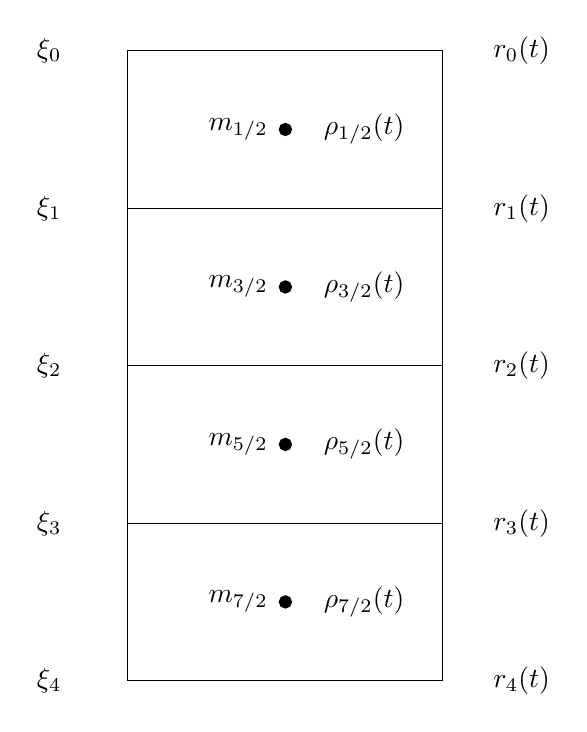
\begin{tikzpicture}[scale=2]
\coordinate (O) at (0,0);
%\draw[semithick](0,0) -- (4,5);
%\draw[semithick](0,0) -- (-4,5);
%\draw[semithick] (4,5) arc (45:135:6.4031242374328485);
\draw (0,0) rectangle (2,1);
\draw (0,1) rectangle (2,2);
\draw (0,2) rectangle (2,3);
\draw (0,3) rectangle (2,4);
%%%
%\draw (-0.5,2.5) -- (-0.5,4.5);
%\draw (6.5,2.5) -- (6.5,4.5);
% xi labels basic nodes
\node at (-0.5,4) {$\xi_0$};
\node at (-0.5,3) {$\xi_1$};
\node at (-0.5,2) {$\xi_2$};
\node at (-0.5,1) {$\xi_3$};
\node at (-0.5,0) {$\xi_4$};
% xi labels staggered nodes
\node at (0.7,3.5) {$m_{1/2}$};
\node at (0.7,2.5) {$m_{3/2}$};
\node at (0.7,1.5) {$m_{5/2}$};
\node at (0.7,0.5) {$m_{7/2}$};
% rho labels staggered nodes
\node at (1.5,3.5) {$\rho_{1/2}(t)$};
\node at (1.5,2.5) {$\rho_{3/2}(t)$};
\node at (1.5,1.5) {$\rho_{5/2}(t)$};
\node at (1.5,0.5) {$\rho_{7/2}(t)$};
% r labels basic nodes
\node at (2.5,4) {$r_0(t)$};
\node at (2.5,3) {$r_1(t)$};
\node at (2.5,2) {$r_2(t)$};
\node at (2.5,1) {$r_3(t)$};
\node at (2.5,0) {$r_4(t)$};
% staggered points
\draw[black,thick,fill=black] (1,3.5) circle [radius=1pt] ;
\draw[black,thick,fill=black] (1,2.5) circle [radius=1pt] ;
\draw[black,thick,fill=black] (1,1.5) circle [radius=1pt] ;
\draw[black,thick,fill=black] (1,0.5) circle [radius=1pt] ;
\end{tikzpicture}
\end{center}
\caption{Schematic representation of the mesh with mass coordinate ($\xi$) or radius $r$ as the spatial dimension.}
\end{figure}
\subsubsection{Relationship to volume (new approach)}
\begin{itemize}
\item We consider elements/cells with fixed mass.
\item Mass of each element is known (prescribed).
\item \textbf{An approximation: hydrostatic/total pressure $P$ is fixed during magma ocean evolution.}  \dbnote{Clearly fails for accreting planet scenario, but in the simplest case can update the hydrostatic pressure each timestep using the same simple EOS as we currently do.}
\begin{itemize}
\item Already in SPIDER, since define radius coordinates and corresponding pressures once during the initialisation.  See Eq.~16 in \cite{BSW18}.
\item We do not recompute the pressure profile due to the evolution of melt fraction (and hence relative contributions of melt versus solid densities) during a model run.
\item Or similarly, it's the differences of melt and solid thermophysical properties at a given pressure, rather than the absolute pressure itself, that is most important for driving the flow.
\item Argument is that melt and solid densities are similar enough to not strongly influence an integrated quantity like pressure.
\item And from a purely pragmatic perspective, we have to know $P$ and $S$ at basic and staggered nodes in order to compute necessary terms for the RHS.
\end{itemize}
\item In the simple case outlined above, we compute density, pressure, and mass by an Adams-Williamson EOS (Eq.~16 in \cite{BSW18}).  \dbnote{Therefore, even for a radial mesh the volume was fixed and also the density, and hence the mass!  Does this partly justify ignoring the convective derivative term in the original formulation?!}
\item More can probably be done here about integrating the hydrostatic .equilibrium equation (see Sect.~\ref{sect:hydrostatic})
\item So assuming we can reasonably determine $P$, and prescribe an initial $S$, we can compute $\rho(P,S)$ at all basic and staggered mesh locations.  \textbf{Knowing $\rho$ and the mass of the elements, and presumably a fixed integration point for $r$ such as the CMB, we can determine the volume of each cell and also the surface areas of the bounding surfaces.}
\item But this could highlight a problem!  Since integrating outwards from the CMB, or inwards from the surface, will not necessarily give us the correct end point of the present-day Earth (since the radius of the surface and core are known well!).
\item \textbf{Two options: switch to test each?}
\begin{enumerate}
\item Assume density of a mass cell is \textbf{constant with time}, i.e. does not respond to changes in melt/solid fraction.  Therefore the volume of the cell will also be constant, and hence the bounding surfaces should correspond to \textbf{time-independent radii}
\item Compute the density of a mass cell, since $\rho(P,S)$ using melt and solid lookup data.  This will result in \textbf{time-dependent radii} for the bounding surfaces, and effectively a planet that can `breathe''.  This might look a bit strange since a planet's surface will move radially in and out as the melt fraction evolves.  \dbnote{And the uncertainties in the EOS, in addition to the overall simplicity of the modelling, probably means this effect is really not important or worthy of modelling (in the case of a fully formed planet).}
\end{enumerate}
\item If we do 1 above, then I think this corresponds closely (or exactly) to the incorrect formulation in the paper?!  Since in both the formulation with $r$ (original) and $\xi$ (new) the bounding surfaces of the elements are assumed to be fixed in time meaning that $\frac{\partial r}{\partial t} = U=0$.  And hence the barycentric velocity is zero and we are justified/consistent when we exclude it from the equation.
\end{itemize}
%%%%%
%%%%%
%%%%%
\section{Hydrostatic equilibrium}
\label{sect:hydrostatic}
\begin{equation}
\frac{dp(r)}{dr} = g(r) \rho(r) = -G \frac{M(r)}{r^2}\rho(r)
\end{equation}
Multiply by $r^2/\rho$ and differentiate with respect to $r$:
\begin{equation}
\frac{d}{dr} \left( \frac{r^2}{\rho(r)} \frac{dp(r)}{dr} \right) = -G \frac{dM(r)}{dr} = -G 4 \pi r^2 \rho(r)
\end{equation}
Rearranging this becomes:
\begin{equation}
\frac{1}{r^2} \frac{d}{dr} \left( \frac{r^2}{\rho}\frac{dp}{dr} \right) = -4 \pi G \rho
\end{equation}
Combined with an EOS of the form $p=p(\rho)$, this is an ordinary second order differential equation for the density or pressure.
%%%%%
%%%%%
%%%%%
\section{Eq. in \cite{ABE93}}
The conversion to mass units means that the Lagrangian derivative becomes the partial derivative:
\begin{equation}
\frac{\partial \omega_i}{\partial t} = -4 \pi \frac{\partial}{\partial m} r^2 \left[ \frac{1-K_i}{K_i+(1-K_i)\phi} \omega_i J_{gm} - \rho \kappa_c \frac{\partial \omega_i}{\partial r} \right]
\end{equation}
%%%%%
%%%%%
%%%%%

\section{Viscosity}
Currently, the standard Arrhenius law is implemented. In order to pin the viscosity to a reference viscosity $\eta_0$ at a certain pressure $P_0$ and temperature $T_0$, it is used in the following form:
\begin{equation}
\ln ( \eta (P,T)) = \ln \eta_0 + \frac{E_a + V_a*P}{RT} - \frac{E_a + V_a P_0}{R T_0},
\end{equation}
for activation energy $E_a$ and activation volume $V_a$. This can be rewritten as
\begin{equation*}
\ln ( \eta (P,T)) = \ln \eta_0 + \frac{(E_a + V_a*(P_0 + \Delta P))*T_0 - (E_a + V_a*P_0)*(T_0 + \Delta T)}{R T_0 (\Delta T + T_0)}
\end{equation*}
for $\Delta P = P - P_0$ and $\Delta T = T - T_0$. If we write $\Delta T' = \Delta T/T_0$, we get
\begin{equation}
\ln ( \eta (P,T)) = \ln \eta_0 + \frac{V_a \Delta P - (E_a + V_a P_0)\Delta T'}{R T_0 (1 + \Delta T')}.
\end{equation}
Values can be specified in the input file, where $\eta_0$ should be specified in -log10visc\_sol, $P_0$ in -P0\_visc and $T_0$ in -T0\_visc. Currently, they are set to CMB values with $\eta0 = 10e22$, $T_0 = T_{CMB} \approx 4000$K and $P_0 = P_{CMB} \approx 138$ GPa. Can also mimic StagYY, where it is set to $P_0 = 0$, $T_0 = 1600$ and $\eta_0 = 10e19$.

\subsection{Compositionally dependent viscosity}
Viscosity is strongly dependent on the Si-abundance in the mantle. Very Si-rich mantles are much more viscous than very Mg-rich mantles. The compositional dependency is applied simply by adding a term to the viscosity, $\ln \eta_{new} = \ln \eta + \Delta \eta_c$. It depends on the Mg/Si-ratio, which is specified in the input file with -Mg\_Si, where you can enter 0.0 to switch it off. Usually, it is set to 1.08, the value for Earth. It is linearly dependent on Mg/Si in several steps:
\begin{equation}
\Delta \eta_c = 
\begin{cases}
2 & \text{Mg/Si} < 0.5 \\
\log(3.3) + (2 - \log(3.3))\frac{0.7 - \text{Mg/Si}}{0.2} & 0.5 \leq \text{Mg/Si} < 0.7 \\
\log(3.3)\frac{1 - \text{Mg/Si}}{0.3} & 0.7 \leq \text{Mg/Si} < 1.0 \\
\log(0.033)\frac{\text{Mg/Si}-1}{0.25} & 1.0 \leq \text{Mg/Si} < 1.25 \\
-2 + (\log(0.033) + 2)\frac{1.5 - \text{Mg/Si}}{0.25} & 1.25 \leq \text{Mg/Si} < 1.5 \\
-2 & \text{Mg/Si} \geq 1.5
\end{cases}.
\end{equation}
%It is centered around Mg/Si=1 here, but can easily be centered around different Mg/Si values by subtracting $\Delta \eta_c$ for the reference Mg/Si from the actual number. It is recommended to center it around the Mg/Si ratio of Earth (which is currently the case) so a viscosity profile based on Earth can be used.
The correction above is centered around Mg/Si = 1.0. If the reference viscosity profile is not for a planet with Mg/Si=1.0, then the compositional correction should be altered to compensate for the difference. This is done by subtracting the compositional correction of the composition for which the reference viscosity profile is calculated (usually Earth-like composition). The composition for which the reference viscosity profile has been calculated can be given in the options file as -Mg\_Si\_ref. This should be set to Earth-like composition as default, since most reference viscosity profiles are calculated for Earth. The compositional correction is stored in P visc\_ref\_comp.

\subsection{Depth-dependent activation volume}
Activation volume $V_a$ changes with depth. This change is already implemented in StagYY, and now also in SPIDER. The implementation and numbers are based on Antoine Rozel's paper, Continental crust formation on early Earth controlled by intrusive magmatism (Nature, 2017). It is described by
\begin{equation}
V_a(P) = V_0 \exp(- P/P_i),
\end{equation}
where $V_0$ is the same as the value for $V_a$ used before, and pressure scaling $P_i$ is given by Rozel et al.\ at $P_i=200$GPa in the lower mantle, and zero in the upper mantle. Currently, in SPIDER it is not possible yet to vary this value between UM and LM (or between layers), but that should not be difficult to implement. Currently, this part is controlled by two input parameters: -activation\_volume\_pressure\_dependency is used to switch this formula on or off (1 is on, any other integer is off), while -activation\_volume\_pressure\_scaling gives the scaling pressure $P_i$ for if the dependency is switched on. Currently it is set to 200e9 Pa (200 GPa).


Using this description for $V_a$ changes the equation for viscosity from equation \ref{eq:visc_constVa}, since the $V_a$ multiplied with $P$ is not the same as the one multiplied with $P_0$ in equation \ref{eq:visc_viscstep1}. Starting from the latter equation, we get
\begin{equation*}
\ln ( \eta (P,T)) = \ln \eta_0 + \frac{( V_a(P)*(P_0 + \Delta P))*T_0 -  V_a(P_0)*P_0*(T_0 + \Delta T) + E_a (T_0 - (T_0 + \Delta T))}{R T_0 (\Delta T + T_0)},
\end{equation*}
which can be slightly rewritten to the form which is implemented in SPIDER,
\begin{equation}
\ln ( \eta (P,T)) = \ln \eta_0 + \frac{V_a(P) \Delta P + P_0 \left( V_a(P) - V_a(P_0) (1 + \Delta T' ) \right) - E_a \Delta T' }{R T},
\label{eq:visc_varVa}
\end{equation}
since $T = T_0(1 + \Delta T' )$. Also, $V_a(P_0) =\exp(-P_0/P_i)$ is a constant throughout the simulation.

\section{Mixing length profile}
According to Kamata (2018) and Wagner et al.\ (2019), the classical mixing length profile is not able to reproduce realistic results, with Nusselt number and average temperature deviating by up to 60\% from 3D simulations. They came up with a way of parametrizing the mixing length profile to get more realistic results. For mantle thickness $D$, the profile can be characterized by two parameters: depth $a$ and size$b$, where the peak of the profile is at a depth of $a\cdot D$ km, and the size of the peak is $b \cdot D$ km. The profile consists of two linear lines from 0 at the top and bottom of the mantle to the peak of the profile. In the classical MLT, we have $a=b=0.5$. Kamata (2018) and Wagner et al. (2019) varied these numbers in their simulations to see which sets gives the most representative results.

\subsection{Kamata's results}
Kamata (2018) finds that the coefficients $a$ and $b$ depend on two parameters: relative mantle size $f = R_{CMB}/R_{top}$, which is about 0.55 for Earth (and is an input parameter for SPIDER), and viscosity contrast across the mantle $\gamma = \ln (\eta_{top}/\eta_{bottom})$.  His descriptions for the parameters are quadratic equations of $f$, $a,b = a_2,b_2 f^2 + a_1,b_1f + a_0,b_0$, where the coefficients depend on $\gamma$. (see equations 13-20 in his paper). He finds that the coefficients slightly depend on the Rayleigh number of the system, but not significantly enough to include it in the parametrization (see Figure 4 in his paper).

\subsection{Wagner et al.'s results}
Wagner et al.\ (2019) use a different parametrization in terms of $\alpha$ and $\beta$, which can be transformed to the original coefficients as $a = \beta/2$ and $b=\alpha/2$. They find a more complex relationship, which depends on the viscosity contrast and on the Rayleigh number of the system. They present a scaling law in their Figure 7 and Table 4,
\begin{equation}
\alpha = \left( a_0 - a_1 \gamma - a_2 \log(\text{Ra}) \right) \tanh \left( a_3 \log (\text{Ra}/\text{Ra}_c) \right),
\end{equation}
where Ra$_c$ is the critical Rayleigh number (which they present an approximation for as a function of $\gamma$). Their parametrization of $\beta$ depends on the dynamic regime. For the stagnant lid regime it is slightly simpler:
\begin{equation}
\beta = b_0 - b_1 \gamma - b_2 \log (\text{Ra}),
\end{equation}
while for the mobile and sluggish lids it's a more complex equation
\begin{equation}
\beta = b_0 - b_1  \tanh \left( \log(\text{Ra}) - b_2 - b_3 \gamma^{b_4} \right).
\end{equation}
Values for the numbers are given in their Table 4, for both Bottom-heated and Mixed heated models (as long as internal heating by radiogenic elements is switched on, we're in the mixed heating regime).

%\section{Parameterised fluxes}
%\subsection{Mixing length theory}
\dbnote{The sign convention needs checking, and may be different to what is actually used in the code.}
Heat (and mass) transport for both the viscous (solid-state) and inviscid regime is parameterised using \textbf{mixing length theory}.  1-D thermal evolution can be effectively modelled using mixing length theory to approximate the radially averaged results of full 3-D convective simulations.  The physical picture is that convective heat transport at a distance $l$ from the nearest boundary is dominated by fluid parcels of size $l$, which transport heat vertically over a distance equal to their size before they dissipate.  The sensible heat flux is expressed as a sum of conductive and convective terms:
\begin{equation}
J_q = -\rho C_p \kappa \left( \frac{\partial T}{\partial r} \right)_S - \rho C_p \kappa_{\rm h}\Delta (\delta_r T)_S
\label{eqn:Jq}
\end{equation}
where $r$ is the radius, $\kappa$ is the thermal diffusivity (due to conduction), $\kappa_{\rm h}$ is the eddy diffusivity (due to convection), and the thermal gradient relative to the adiabat is given by:
\begin{equation}
\label{eqn:thermgrad}
\Delta (\delta_r T)_S =  \frac{\partial T}{\partial r} - \left( \frac{\partial T}{\partial r} \right)_S 
\end{equation}
Equation \ref{eqn:Jq} is cast in a diffusive form identical to Fourier's Law, where the adiabatic thermal gradient transports heat according to simple conduction, and the deviation from the adiabat carries heat diffusively through either conduction, viscous convection, or inviscid convection, as appropriate (for details, see section \ref{sec:mixinglenth} below).

The effective convective diffusivity is expressed in a form identical to Fourier's law (formerly called the eddy diffusivity according to Abe 1993), is determined from the mean free path by $\kappa \sim v l$:
\begin{equation}
  \kappa_{\rm conv} = \begin{cases}
  0 & \Delta(\delta_z T)_S \leq 0 \\
  v_{\rm vis}l & 0 < {Re}_{\rm loc} < 9/8 \\
  v_{\rm invis}l &  9/8 \leq { Re}_{\rm loc}
\end{cases}
\label{eq:convdiff}
\end{equation}
where stable stratification prevents convection when the temperature gradient is not as steep as the adiabat ($\Delta(\delta_z T)_S \leq 0$), and otherwise the local Reynolds number $Re_{\rm loc} = v_{\rm vis} l / \nu$ determines the importance of viscosity to the resulting convection.
The convective velocities are given by a balance of the buoyancy force on each fluid parcel against the viscous drag or pressure drag forces, in the viscous and inviscid cases, respectively:
\begin{equation}
  v_{\rm vis} = \frac{\alpha |g| l^3}{18\nu}  \Delta(\delta_z T)_S \\
\end{equation}
\begin{equation}
  v_{\rm invis} = \sqrt{\frac{\alpha |g| l^2}{16}  \Delta(\delta_z T)_S} \\
\end{equation}
For viscous convection, the parcel velocity is given by Stokes settling for a sphere of diameter $l$. The inviscid case can be determined up to a constant by equating the dynamic pressure force $\sim$$\rho v^2$ with the buoyancy force \awnote{though the exact source of the proportionality constant is unknown}.



To remain consistent with the entropy-pressure formulation used in this study (and avoid the accumulation of numerical errors caused by converting back and forth between entropy and temperature space), we must rewrite the heat transport expressions in terms of entropy gradients, rather than temperature gradients.
The temperature gradient is given by the total differential with respect to pressure and entropy:
\begin{equation}
  \frac{dT}{dr} = \left( \frac{\partial T}{\partial S}\right)_P \frac{dS}{dr} + 
  \left( \frac{\partial T}{\partial P}\right)_S \frac{dP}{dr}
\end{equation}
where the total derivatives $dT\big/dr$, $dS\big/dr$, and $dP\big/dr$, simply reflect the observed gradients along the current temperature, entropy, and pressure profiles of the system, respectively.
Thus, we can rewrite the thermal gradient relative to the adiabat as:
\begin{equation}
\label{eqn:thermgrad_s}
\Delta (\delta_r T)_S =   \left( \frac{\partial T}{\partial S}\right)_P \frac{dS}{dr} = 
\frac{T}{C_p} \frac{dS}{dr}
\end{equation}
yielding a simple expression in terms of the observed radial profile of entropy, rather than temperature.
By substituting into the heat flux expression from Equation \ref{eqn:Jq}, we obtain:
\begin{equation}
  J_q =-\rho C_p \kappa \left( \frac{\partial T}{\partial P}\right)_S \frac{dP}{dr} -
  \rho \kappa_{\rm h} T \frac{dS}{dr}
\label{eqn:Jq_s}
\end{equation}
which enables evaluation of the heat flux directly in pressure-entropy space.


\subsection{Mixing Length Theory}
\label{sec:mixinglenth}

\awnote{ The primary difference between this formulation of mixing length theory and Abe's is that Abe allows convection to ``turn on'' instantly, where it contributes to the total heat transport as soon as the temperature goes super adiabatic. I believe this is WRONG, because it includes additional heat transport due to convection even within a thermal boundary layer (where only conduction operates). Instead, this slight modification ensures that only conduction operates within both stably stratified regions (low thermal gradient) and thermal boundary layers (high thermal gradient), reflecting the fact that convection is inhibited in both these regions, though for different reasons. This formulation also allows interior thermal boundary layers to arise naturally, without crossing any discontinuities in terms of the heat flux. }

The heat-transport diffusivity (formerly called the eddy diffusivity according to Abe 1993) is a piecewise function depending on the heat-transport regime:
\begin{subnumcases}{\kappa_h=}
  \kappa & $\kappa_{\rm vis} \le \kappa \label{eqn:convdiff_a}$ \\
  \kappa_{\rm vis}  & $\kappa < \kappa_{\rm vis} < \nu$  \label{eqn:convdiff_b} \\
  \kappa_{\rm invis} & $\nu \leq \kappa_{\rm vis} \label{eqn:convdiff_c}$
\end{subnumcases}
Viscous diffusive heat transport is the norm for planetary convection, where the rise and fall of convective parcels is primarily resisted by viscous drag (corresponding to Stokes settling).
Within both thermal boundary layers and stably stratified regions, thermal diffusion dominates, where conduction transports heat faster than convection ($\kappa_{\rm vis} \le \kappa$), thereby damping the growth of convective instabilities.
In highly turbulent systems, viscous diffusivity can exceed the viscosity ($\nu \le \kappa_{\rm vis}$), implying that dynamic pressure (not viscous drag) is the dominant force resisting the vertical transport of convective parcels, and thus the system adopts the inviscid diffusivity.
\awnote{Abe 1993 places the boundary between viscous and inviscid convection at $9/8 \cdot \nu$ rather than at $1 \cdot \nu$, but I see no strong justification for this.}


In either convective regime, we estimate the appropriate diffusivity using the average mean-free-path of convective parcels:
\begin{equation}
\kappa_{\rm conv} \sim v_{\rm conv} l
\end{equation}
where $l$ is the convective mixing length, assumed to be equal to the distance to the core of the nearest boundary layer, corresponding to either the top or bottom of the convecting system, or the center of any interior thermal boundary layers that arise as the system evolves.

\subsubsection{Viscous scaling}
For the viscous case, we balance of the buoyancy force on each fluid parcel against the viscous drag:
\begin{equation}
F_{\rm drag} = \frac{1}{2} \rho_{\rm F} U^2 C_{\rm D} A
\end{equation}
where $\rho_{\rm F}$ is density of the fluid, $U$ is velocity, $C_{\rm D}$ is drag coefficient, and $A$ is drag area.
For low laminar flow at low concentrations of perfectly spherical particles and low Reynolds number:
\begin{equation}
C_{\rm D} = 24 / Re = \frac{24 \nu}{U l}
\end{equation}
where $\nu$ is kinematic viscosity, and $l$ is an appropriately chosen length-scale.
\begin{figure}[!bthp]
\centering
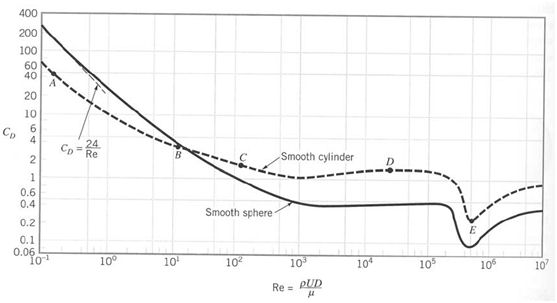
\includegraphics[width=1.0\textwidth]{figs/Shape_CoefficientC.jpg}
\caption{Drag coefficient as a function of Reynolds number for a smooth cylinder and a smooth sphere.  The linear approximation of $24/Re$ is also shown.  (Stolen from the internet so beware of copyright!)}
\end{figure}
Therefore,
\begin{equation}
F_{\rm drag} = 12 \nu \rho_{\rm F} U A / l
\end{equation}
Substituting in the drag area of a sphere:
\begin{equation}
F_{\rm drag} = 12 \nu \rho_{\rm F} U \pi (d/2)^2 / l
\end{equation}
where $d$ is the particle diameter.
The force that balances the drag force is the buoyancy force:
\begin{equation}
12 \nu \rho_{\rm F} U \pi (d/2)^2 / l = \frac{4}{3} \pi \left(\frac{d}{2}\right)^3 g (\rho_{\rm S} - \rho_{\rm F})
\end{equation}
where $g$ is gravitational acceleration, and $\rho_{\rm S}$ is density of the spherical particle.  Rearranging:
\begin{equation}
U = \frac{gdl}{18 \nu} \left( \frac{\rho_{\rm S} - \rho_{\rm F}}{\rho_{\rm F}} \right)
\end{equation}
The fractional density difference due to thermal effects can be expressed as: \dbnote{TODO: this should have factor of 1/2 I think}
\begin{equation}
\frac{\rho_{\rm S} - \rho_{\rm F}}{\rho_{\rm F}} = \alpha \Delta T = \alpha l \left( \frac{dT}{dz} - \left( \frac{dT}{dz} \right)_{\rm s} \right)
\end{equation}
And finally, set the particle diameter equal to the length-scale parameter $l$, which is the mixing length: \dbnote{TODO: also need to introduce factor of 1/2 from averaging over mixing length}
\begin{equation}
U = \frac{\alpha g l^3}{18 \nu} \left( \frac{dT}{dz} - \left( \frac{dT}{dz} \right)_{\rm s} \right)
\end{equation}
%%%%
%%%%
%%%%
\subsubsection{Inviscid scaling}
For the inviscid case we follow \citep{V53}, with some additional insights from \cite[p. 50,][]{KWW12}.  Kinetic energy of a fluid element is balanced by the work done by the buoyancy force over some length scale $x$:
\begin{equation}
\frac{1}{2} m v^2 = \int_0^x K(x) dx
\end{equation}
where $x$ relates to the mixing length.  The buoyancy force is:
\begin{equation}
K(x) = V g \Delta \rho(x) = m g \alpha \Delta T(x)
\end{equation}
where $V$ is volume of the element, $g$ gravity, $\Delta \rho$ density anomaly, $m$ mass of the element, $\alpha$ thermal expansion coefficient, $\Delta T$ thermal anomaly:
\begin{equation}
\Delta T(x) = \left( \frac{dT}{dz} - \left( \frac{dT}{dz} \right)_s \right) x
\end{equation}
Now we can integrate:
\begin{equation}
\int_0^x K(x) dx = mg \alpha  \left( \frac{dT}{dz} - \left( \frac{dT}{dz} \right)_s \right) \frac{x^2}{2}
\end{equation}
Putting this together with the kinetic energy \citep[Eq.~5,][]{V53}:
\begin{equation}
v(x) = \sqrt{\alpha g x^2 \left( \frac{dT}{dz} - \left( \frac{dT}{dz} \right)_s \right)}
\label{eq:mixvele}
\end{equation}
This establishes the basic form of the inviscid scaling for velocity, minus the factors of two that are now discussed.  \cite{V53} then computes an average velocity of all the parcels of fluids with different mixing lengths that are passing through the same region:
\begin{equation}
\overline{v} = \frac{\int_0^l v dx}{\int_0^l dx} = \sqrt{\frac{\alpha g l^2}{4} \left( \frac{dT}{dz} - \left( \frac{dT}{dz} \right)_s \right)}
\end{equation}
This agrees with \cite[Eq.~6a,][]{V53}.  Note that in \cite{V58} she increases the factor from 4 to 8 to improve the description of the turbulent friction \citep[see][]{B98}.  \cite{HVB65} actually look at values up to 16, which may perhaps be the origin of the factor of 16 in \cite{ABE93,ABE95}?  Other origins for factors of two include considering the average thermal perturbation of an element over $[0,x]$:
\begin{equation}
\overline{\Delta T} = \frac{\int_0^l \Delta T dx}{\int_0^l dx} = \left( \frac{dT}{dz} - \left( \frac{dT}{dz} \right)_s \right) \left( \frac{l}{2} \right)
\end{equation}
\cite{KWW12} consider an ``average'' element from the start of their derivation, and thus introduce a factor of two through the average path length of $l_m/2$, which first appears in the thermal anomaly.  Second, another factor of two appears since the buoyancy force is integrated over the average path length.  Finally, another factor of two appears since they assume that half of the work goes into the kinetic energy of the element.  Hence \cite{KWW12} end up with a factor of 8 in the denominator, albeit by slightly different reasoning.  Although \cite{ABE93,ABE95} reference \cite{V53}, it's not obvious that you can just use \cite{V53} and arrive with a factor of 16 in the denominator.  Since factors of 2 seem to be introduced for a variety of reasons by different authors, with origins that are not necessarily explained well, we may just have to accept that \cite{ABE93,ABE95} uses a factor of 16 in the denominator by appealing to a combination of the reasons previously described.  In the end, the numerical challenges result from the presence of the square-root and not the constant prefactor:
\begin{equation}
v_{\rm invis} = \sqrt{\frac{\alpha g l^2}{16} \left( \frac{dT}{dz} - \left( \frac{dT}{dz} \right)_s \right)}
\end{equation}

%%% added Rob Spaargaren as part of his MSc work
\subsection{Kamata and Wagner profile}
According to Kamata (2018) and Wagner et al.\ (2019), the classical mixing length profile is not able to reproduce realistic results, with Nusselt number and average temperature deviating by up to 60\% from 3D simulations. They came up with a way of parametrizing the mixing length profile to get more realistic results. For mantle thickness $D$, the profile can be characterized by two parameters: depth $a$ and size$b$, where the peak of the profile is at a depth of $a\cdot D$ km, and the size of the peak is $b \cdot D$ km. The profile consists of two linear lines from 0 at the top and bottom of the mantle to the peak of the profile. In the classical MLT, we have $a=b=0.5$. Kamata (2018) and Wagner et al. (2019) varied these numbers in their simulations to see which sets gives the most representative results.

\subsubsection{Kamata's results}
Kamata (2018) finds that the coefficients $a$ and $b$ depend on two parameters: relative mantle size $f = R_{CMB}/R_{top}$, which is about 0.55 for Earth (and is an input parameter for SPIDER), and viscosity contrast across the mantle $\gamma = \ln (\eta_{top}/\eta_{bottom})$.  His descriptions for the parameters are quadratic equations of $f$, $a,b = a_2,b_2 f^2 + a_1,b_1f + a_0,b_0$, where the coefficients depend on $\gamma$. (see equations 13-20 in his paper). He finds that the coefficients slightly depend on the Rayleigh number of the system, but not significantly enough to include it in the parametrization (see Figure 4 in his paper).

\subsubsection{Wagner et al.'s results}
Wagner et al.\ (2019) use a different parametrization in terms of $\alpha$ and $\beta$, which can be transformed to the original coefficients as $a = \beta/2$ and $b=\alpha/2$. They find a more complex relationship, which depends on the viscosity contrast and on the Rayleigh number of the system. They present a scaling law in their Figure 7 and Table 4,
\begin{equation}
\alpha = \left( a_0 - a_1 \gamma - a_2 \log(\text{Ra}) \right) \tanh \left( a_3 \log (\text{Ra}/\text{Ra}_c) \right),
\end{equation}
where Ra$_c$ is the critical Rayleigh number (which they present an approximation for as a function of $\gamma$). Their parametrization of $\beta$ depends on the dynamic regime. For the stagnant lid regime it is slightly simpler:
\begin{equation}
\beta = b_0 - b_1 \gamma - b_2 \log (\text{Ra}),
\end{equation}
while for the mobile and sluggish lids it's a more complex equation
\begin{equation}
\beta = b_0 - b_1  \tanh \left( \log(\text{Ra}) - b_2 - b_3 \gamma^{b_4} \right).
\end{equation}
Values for the numbers are given in their Table 4, for both Bottom-heated and Mixed heated models (as long as internal heating by radiogenic elements is switched on, we're in the mixed heating regime).


%\section{Derivations in Abe (1993)}
%\fbox{\parbox{\textwidth}{Notes that are specific to the derivations in \cite{ABE93}}}

\subsection{Phase Separation}
Under the assumption of no melting/solidification, melt-solid separation is treated merely as a mass-transfer process in a two-phase mixture.  Average density of mixture given by:
\begin{equation}
\frac{1}{\rho} = \frac{1}{\rho_s}(1-\phi)+\frac{1}{\rho_m}\phi
\label{eq:abe1993_rho}
\end{equation}
where $\phi$ is mass fraction of melt.
The masses of solid and melt phases per unit volume of mixture (or spatial density of solid and melt phase) are:
\begin{equation}
\rho_s^\ast \equiv (1-\phi) \rho = \frac{\rho_s \rho_m (1-\phi)}{\rho_s \phi + \rho_m(1-\phi)}
\label{eq:abe1993_rhos}
\end{equation}
\begin{equation}
\rho_m^\ast \equiv \phi \rho = \frac{\rho_s \rho_m \phi}{\rho_s \phi + \rho_m(1-\phi)}
\label{eq:abe1993_rhom}
\end{equation}
Mass conservation of each phase in a 1-D system (no melting/solidification):
\begin{equation}
\frac{\partial \rho_m^\ast}{\partial t} + v_m \frac{\partial \rho_m^\ast}{\partial z} = -\rho_m^\ast \frac{\partial v_m}{\partial z}
\end{equation}
\begin{equation}
\frac{\partial \rho_s^\ast}{\partial t} + v_s \frac{\partial \rho_s^\ast}{\partial z} = -\rho_s^\ast \frac{\partial v_s}{\partial z}
\end{equation}
$v_m$ and $v_s$ are velocities averaged over a small domain in the mixture.  $z$ increases upwards.
Define the velocity of the local barycenter of the mixture, $v$, 
\begin{equation}
v \equiv \frac{\rho_m^\ast}{\rho_m^\ast + \rho_s^\ast} v_m + \frac{\rho_s^\ast}{\rho_m^\ast + \rho_s^\ast} v_s = \phi v_m + (1-\phi) v_s
\end{equation}
enabling us to write the mass conservation equation for the system as a whole:
\begin{equation}
\frac{\partial \rho}{\partial t} + v \frac{\partial \rho}{\partial z} = -\rho \frac{\partial v}{\partial z}
\end{equation}
We also define the vertical mass flux of melt, $J_m$, relative to the local barycenter (characterizes the melt-solid separation processes):
\begin{equation}
J_m \equiv \rho_m^\ast (v_m-v) = \rho \phi (1-\phi)(v_m-v_s)
\end{equation}
Using $v$ and $J_m$:
\begin{equation}
v_m = v + \frac{J_m}{\rho \phi}
\end{equation}
\begin{equation}
v_s = v - \frac{J_m}{\rho (1-\phi)}
\end{equation}
Substituting above 2 equations into mass conservation equations (product and chain rule differentiation, then cancel terms):
\begin{equation}
\frac{\partial \rho_m^\ast}{\partial t} + v \frac{\partial \rho_m^\ast}{\partial z} = -\rho_m^\ast \frac{\partial v}{\partial z} - \frac{\partial J_m}{\partial z}
\label{eq:abe1993_rhom_star}
\end{equation}
\begin{equation}
\frac{\partial \rho_s^\ast}{\partial t} + v \frac{\partial \rho_s^\ast}{\partial z} = -\rho_s^\ast \frac{\partial v}{\partial z} + \frac{\partial J_m}{\partial z}
\label{eq:abe1993_rhos_star}
\end{equation}
We can expand the LHS of equation \ref{eq:abe1993_rhom_star} (using substitution for $\rho_m^\ast=\phi\rho$, the product rule, and the application of mass conservation for the total mixture):
\begin{equation}
  \rho(\frac{\partial \phi}{\partial t} + v \frac{\partial \phi}{\partial z}) + \phi(\frac{\partial \rho}{\partial t} + v \frac{\partial \rho}{\partial z})= \rho(\frac{\partial \phi}{\partial t} + v \frac{\partial \phi}{\partial z})  - \phi\rho \frac{\partial v}{\partial z}
\end{equation}
Canceling the repeated term from the RHS and dividing by $\rho$, we get:
\begin{equation}
\frac{\partial \phi}{\partial t} + v \frac{\partial \phi}{\partial z} = - \frac{1}{\rho} \frac{\partial J_m}{\partial z}
\label{eq:abe1993_phaseSepPart1}
\end{equation}
From Equation \ref{eq:abe1993_rho}, we can rewrite $\phi$ in terms of $\rho$ and material constants:
\begin{equation}
\phi = \frac{\rho_m ( \rho_s - \rho)}{\rho ( \rho_s-\rho_m)}
\end{equation}
We can then simplify the L.H.S. of Equation \ref{eq:abe1993_phaseSepPart1} using the chain rule:
\begin{equation}
  \frac{\partial \phi}{\partial t} + v \frac{\partial \phi}{\partial z} = 
  \frac{\partial \phi}{\partial \rho} ( \frac{\partial \phi}{\partial t} + v \frac{\partial \rho}{\partial z}) = 
  -\rho \frac{\partial \phi}{\partial \rho}\frac{\partial v}{\partial z}
\label{eq:abe1993_phaseSepPart2}
\end{equation}
Assuming that $\rho_m$ and $\rho_s$ are constant and are not functions of depth $z$ (or~$\rho$),
\begin{equation}
\frac{\partial \phi}{\partial \rho} = \frac{\rho_m \rho_s}{\rho^2 (\rho_m-\rho_s)}
\label{eq:abe1993_dphidrho}
\end{equation}
which can be substituted into Equation \ref{eq:abe1993_phaseSepPart2} and combined with Equation \ref{eq:abe1993_phaseSepPart1} to obtain a final expression governing phase separation:
\begin{equation}
\frac{\partial \phi}{\partial t} + v \frac{\partial \phi}{\partial z} = \frac{\rho_m \rho_s}{\rho (\rho_s-\rho_m)} \frac{\partial v}{\partial z}
= - \frac{1}{\rho} \frac{\partial J_m}{\partial z}
\label{eq:abe1993_phaseSep}
\end{equation}

%Working:
%\begin{equation}
%\label{rho}
%\rho = \rho_m^\ast + \rho_s^\ast 
%\end{equation}
%\begin{equation}
%\rho_s^\ast =  \rho-\rho_m^\ast
%\end{equation}
%\begin{equation}
%\rho_m^\ast = \rho \phi
%\end{equation}
%To derive the `main' equation in Abe 1993 you use eqn~\ref{rhosstar} and eqn~\ref{rhomstar}.  To get the expression involving $\partial J_m/\partial z$ (in the main equation) you have to eliminate $\partial v/\partial z$ from equations \ref{rhomstar} and \ref{rhosstar} by combining them.  To do this, you subtract (eqn~\ref{rhosstar} $\times \rho_m^\ast$) from (eqn~\ref{rhomstar} $\times \rho_s^\ast$) and use above substitutions to eliminate $\rho_s^\ast$.  Use product rule to differentiate $(\rho \phi)$ and cancel terms.  Rearrange to give:
%\begin{equation}
%\frac{\partial \phi}{\partial t} + v \frac{\partial \phi}{\partial z} = - \frac{1}{\rho} \frac{\partial J_m}{\partial z}
%\end{equation}
%%%%%
%Now, to get the expression involving $\partial v/\partial z$ in the main equation, you have to combine equations \ref{rhomstar} and \ref{rhosstar} in such a way as to eliminate $\partial J_m/\partial z$.  This is easily done by adding eqn.~\ref{rhomstar} and eqn.~\ref{rhosstar} together.  Then, use eqn~\ref{rho} to combine terms and substitute in eqn~\ref{dphidrho} after applying the chain rule (as follows):
%\begin{equation}
%\frac{\partial \phi}{\partial t} + v \frac{\partial \phi}{\partial z} = - \rho \frac{\partial \phi}{\partial \rho}\frac{\partial v}{\partial z} = \frac{\rho_m \rho_s}{\rho (\rho_s-\rho_m)} \frac{\partial v}{\partial z}
%\label{eq:abe1993_phaseSep}
%\end{equation}
%For a while I went around in circles trying to directly relate $\partial J_m/\partial z$ to $\partial v/\partial z$ and in the end I gave up in favour of simply eliminating the terms using simple addition and subtraction of the equations as outlined above.  This obviously works, which must mean that I was violating some assumptions about mass conversation, or not applying the product or chain rule correctly when trying to get directly from $\partial J_m/\partial z$ to $\partial v/\partial z$.  I never did reach a satisfactory explanation of why I couldn't do it (but interesting to see you ran into the same problem).

\subsection{Time Scale}
Characteristic time scale $\tau$ of melt-solid separation.  Shorter one of the e-folding time of melt fraction or solid fraction change in the lower half of the layer.  Partially molten layer of thickness $L$ with uniform initial melt fraction $\phi_0$.

To separate melt and solid in this half layer, assuming a (representative) mass flux of $J_m$, and a mass fraction of either $\phi$ (melt) or $1-\phi$) (solid):
\begin{equation}
\tau = \frac{\rho L}{2 J_m} \min (\phi_0, 1-\phi_0 )
\end{equation}
\dbnote{Still not 100\% why this is called an e-folding time.  You can derive the characteristic timescale by simply calculating the mass of melt or solid in the volume and a mass flux.  You don't need to solve an equation of the form dA/dt=A which I usually think of as necessary to call it an ``e-folding time''}
Presumably this is referred to as an e-folding time due to the form of the PDE and/or assumed form of the solution (expected exponential decay).  But the timescale is simply a separation time over half the layer thickness.

\subsection{Impact Stirring}
\awnote{Many of the details from this section are missing from Abe (1993), and some of the equations reported there have large errors. This derivation is inferred by combining personal derivation with Abe (1993) and the source papers sited there (e.g. Kieffer(1980), Davies(1985), Holsapple(1982))}

Earth accreted through a series of planetesimal impacts, which had an important effect on magma ocean mixing since each impact stirred the mantle below the impact site.
To gain a first order handle on impact stirring, a simple model is developed assuming a roughly linear accretion rate:
\begin{equation}
\frac{dm}{dt} \sim \frac{M_E}{\tau_{acc}}
\label{eq:abe1993_accrate}
\end{equation}
where $M_E$ is the Earth's mass and $\tau_{acc} \approx 10$~Myr is the assumed total accretion timescale.

Planetesimal impact stirring depends strongly on impactor size, with more massive impactors stirring a mantle region to both a greater depth and over a larger footprint.
To model the impactor masses, we assume a power-law distribution:
\begin{equation}
  \frac{dN}{dm} = {K_{max}\left(\frac{m}{M_{max}}\right)^{-q}}
\end{equation}
where $q=1.5$ describes the relative proportion of large vs small planetesimals, and $M_{max}=0.1 M_E$.
This characteristic mass distribution (with $q<2$), implies that the majority of the Earth was built from large rather than small impactors.
To obtain the value for the constant $K_{max}$, we simply integrate the mass distribution, requiring that the accreted impactors sum to the Earth's total mass, ${M_E = \int_0^{M_{max}} m \frac{dN}{dm}dm}$, yielding:
\begin{equation}
  K_{max} = \frac{2-q}{M_{max}}\left(\frac{M_E}{M_{max}}\right)
\end{equation}
This impactor mass distribution can now be used to determine the effectiveness of impact stirring.

Each impactor is able to stir a region of the Earth's mantle below the impact site, which depends on impact size and velocity.
We consider two overlapping stirred regions: the deep narrow region corresponding to the initial penetration of the impactor itself and the shallow broad region reflecting the resulting impact crater.
\awnote{In reality, this is more complicated since we also consider impacts into a magma ocean. Though this type of impact creates a temporary cavity rather than a semi-permanent crater, the physics of the cavity size are similar to gravity-dominated craters, for which the effect of rock-strength is negligible. Thus, hopefully, we can use the same crater-scaling laws to approximate the dimensions of the transient crater cavity, even for a predominantly molten Earth target.}
By assuming a (simplified) constant accretion rate (Equation \ref{eq:abe1993_accrate}), we can evaluate the depth-dependent impact stirring timescale as a fraction of the total accretion timescale:
\begin{equation}
  \tau_{s}(d) = \frac{\tau_{acc}}{N_{s}(d)}
  \label{eq:abe1993_taustir}
\end{equation}
where $d$ is the depth and $N_{s}$ is the effective number of complete stirring events occurring over the entire accretion period at depth $d$.
The number of stirring events can be approximated as:
\begin{equation}
  N_{s}(d) = \frac{S_s(d)}{4\pi(R_E - d)^2}
\end{equation}
representing simply the ratio of the total stirred area (throughout accretion), $S_s(d)$, to the total planetary area at depth $d$.
\awnote{This is similar to Equation 18 of Abe(1993), but that expression has numerous typos, inverting numerator and denominator and missing a needed factor of 4.}
This neglects the fact that the Earth grows as it accretes, and thus early impacts collide with a smaller planet, effectively stirring to greater depths.
This expression thus produces only a rough stirring timescale that is actually an upper-bound, when combined with Equation \ref{eq:abe1993_taustir}.
The two stirred regions can be evaluated from impact physics. 

Direct impactor penetration stirring produces disrupts a deep narrow region of the mantle, defined by the impactor size and penetration depth:
\begin{eqnarray}
  s_p =& \pi r_i^2 \\
  d_p =& 2 r_i v_i/v_s
\end{eqnarray}
where the stirred penetration area of a single impact, $s_p$, is simply the cross sectional area of the impactor with radius $r_i$, and the penetration depth $d_p$, depends on the impactor velocity $v_i$ and the shock wave speed $v_s$.


Impact crater formation, on the other hand, disrupts a shallow broad region of the mantle:
\begin{eqnarray}
  s_{crat} =& \pi r_{crat}^2 \\
  d_{crat} =& f_{crat} r_{crat}
\end{eqnarray}
where $r_{crat}$ is the crater radius and $f_{crat}=0.4$ is a typical crater depth to radius ratio.
To determine the crater radius, we rely on crater scaling laws from the literature, like those reported in Davies(1985), rewritten in the form of \cite{ABE93} as:
\begin{equation}
  V_{crat} = \pi f_{crat} r_{crat}^3 = B m_i^{1-\beta/3} (v_i^2/g)^{+ \beta}
\end{equation}
which approximates the crater volume as a cylinder and depends on the impactor mass $m_i$, the impactor velocity $v_i$, and gravity $g$.
The scaling parameters $B$ and $\beta$ characterize the physical scaling between these quantities, where this form is appropriate for large gravity-dominated collisions where target strength is unimportant.

The total stirred area is calculated as an integral over the impactor mass distribution:
\begin{equation}
  S_s(d)= \int_0^{M_{max}} s(m)\Theta(m > m_c(d))  \frac{dN}{dm} dm
\end{equation}
where $m_c(d)$ is the critical mass below which craters are unable to stir to beyond depth $d$, and $\Theta()$ is a step function ensuring that only sufficiently large impactors able to stir to great enough depth contribute to the total stirred area.
When evaluating the total stirred area, Abe (1993) calculated separately for crater and penetration stirring, and used only the shortest timescale.
In reality, we should use the large crater footprint for the shallow regime and the narrow penetration footprint for the deep regime, which is accomplished by splitting this into two separate integrals.
\awnote{Need to finish this!}

Examination of impact stirring timescales is that they all exceed the timescale for gravitational separation for melt fractions above $\sim$13\%.
Thus, if the melt fraction remains above 0.2 due to suppression from vigorous convective mixing, then impacts play a negligible role.
\awnote{Need to justify this argument based on python runs and include in section above}

%K_{max} = \frac{(2-q)M_E}{M_{max}^2}

\subsection{Thermal Evolution of a Magma Ocean}
Begin with the energy (enthalpy) balance equation for a spherically symmetric planet in local thermodynamic equilibrium: 
\begin{equation}
  \frac{\partial H}{\partial t} = - \frac{1}{\rho}\nabla \cdot \vec{J_{tot}} + \Delta V_m|g|\vec{J_m} \cdot \hat{r} + q_{heat}
\end{equation}
where this accounts for the imbalance of energy flows into/out-of a spherical shell at constant pressure, combined with the change in potential energy due to melting density differences, and internal heating (units are energy per unit mass per unit time).
\awnote{I think this neglects changes in Press due to mass redistribution, but that is fine since they are small for magma ocean\dots but not so if core formation is also being considered}
Here  $J_{tot}$ is the total heat flux, $J_m$ is the total mass flux of melt, and $q_{heat}$ is the total heat generated at this depth.  $\hat{r}$ is the radial unit vector.
Note that this total heat generation represents a sum over all sources including radioactive and tidal heating.
Similarly, the total melt mass flux results from both gravitational separation and convective mixing, ${J_m = J_{gm} + J_{cm}}$.

We can expand the divergence in spherical coordinates, dropping non-symmetric terms, and converting from radius to depth: 
\begin{equation}
  \frac{\partial H}{\partial t} = - \frac{1}{4\pi r^2 \rho} \frac{\partial L_{tot}}{\partial r} + \Delta V_m|g|J_{m\hat{r}} + q_{heat}
\end{equation}
where $L_{tot} = 4 \pi r^2 J_{tot}$ is the total luminosity (energy transported upwards per unit time) carried upward past the current depth. 
\awnote{Abe(1993) converted this equation from depth to mass coordinates, ${\partial m /\partial r = 4 \pi r^2 \rho}$, though this is somewhat nonintuitive for Earth Science audiences.}

\dbnote{ $\Delta V_m = \frac{1}{\rho_m} - \frac{1}{\rho_s} >0$ right? (for the simple case of a typical solid more dense than its melt).  So with more melt flux radially outward the gravitational potential energy is becoming less negative, hence the $+$ sign in the energy balance - correct?}

The total heat flux is a combination of the sensible and latent heat components:
\begin{equation}
  J_{tot} = J_q + T\Delta S_m J_m
\end{equation}
Here $\Delta S_m$ and $\Delta V_m$ are the entropy and volumes of melting (fusion) and $J_q$ is the direct convective heat flux.
The enthalpy and volumes of melting ${\Delta H_m = T(P, [\phi])\Delta S_m(P)}$ and ${\Delta V_m = \Delta V_m(P)}$ are both pressure-dependent quantities (although the entropy change on melting $\Delta S_m$ is often reasonably approximated as constant).

The enthalpy conservation equation implicitly depends on the melt fraction $\phi$ in many places: the convective heat flux $J_q$ depends strongly on the melt-fraction dependent viscosity $\eta(\phi)$, both convective mixing and gravitational separation ${J_m = J_{gm}(\phi) + J_{cm}(\phi)}$, and total density $\rho(\phi)$.
\awnote{something weird happening with highlighting here\dots}
Also, if tidal heating is being considered, tidal dissipation depends very strongly on viscosity, and is thus $\phi$ dependent.
Also note that the melt flux $J_m$ is formerly equal to zero if $\phi=1$ or $\phi=0$.
\awnote{I am not sure that this is explicitly stated in Abe 1993 anywhere, though it is clearly true!}

The form of the energy balance equation used by Abe1993 was in terms of temperature instead of enthalpy (though I think this is less useful, since it makes evolution of a single component system needlessly difficult).
\begin{equation}
  [C_p  + \Delta h (\frac{\partial \phi}{\partial T})_P] \frac{\partial T}{\partial t}= - 4\pi \frac{\partial}{\partial m} r^2[J_q + \Delta h J_m] + \frac{1}{\rho}(\Delta \rho/\rho)|g|J_m + q_{heat}
\end{equation}

\awnote{This form also relies on the constancy of the heat capacity during partial melting and the LHS is not applicable if the system is either fully molten or fully solid}

We can employ a good approximate expression for the melt fraction:
\begin{equation}
  \phi(H) = \frac{H - H_{sol}}{T\Delta S_m(P)} 
\end{equation}
for $H_{sol} < H < H_{liq}$ and otherwise $\phi = 1$ above the liquidus (or 0 below the solidus).
This expression is exact for single component systems and reasonably accurate for multi-component systems to the extent that the entropy change on melting $\Delta S_m$ has similar values for all solid phases.
This expression replaces the less accurate version in terms of temperature used by Abe 1993 (that further requires equal heat capacities for all solid phases), which is not useful for single component systems where partial melt is pinned to the melting curve.

%\awnote{
%This provides us a way forward considering only a single component bridgmanite mantle:
\begin{itemize}
  \item Use a single component melting curve roughly corresponding to the 50\% solidus line for a realistic mantle chemistry. 
  \item Entropy of melting can be adjusted to ensure solidus and liquidus enthalpy bounds that match the true mantle system. 
  \item Use realistic heat capacity and density values (EOSs) for both solid and liquid phases. 
  \item This relies on 2 approximations: 
    \begin{enumerate}
      \item Chemical differentiation is negligible (second order effect, at least energetically)
      \item The thermal range of the partially molten region ($\sim$200~K) is small compared to the temperature difference across the mantle ($\sim$2500~K). Values from Stixrude(2009).
    \end{enumerate}
  \item Allows us to focus on the role of tidal dissipation at depth for keeping a magma ocean near the critical melt fraction (somewhere between 40\% and 60\%), for extremely long times without having to worry about chemical evolution. 
  \item Later work can more carefully examine multi-component evolution using equations of Abe 1995.
\end{itemize}
%}

The melting curve used by Abe 1993 is from Ohtani (1983). \awnote{though it may be slightly adjusted?}
Ohtani appears to assume a constant entropy change on melting (fairly reasonable assumption) of 8.03 cal/mol/K for MgSiO3 melt.
The enthalpy change in Abe 1993 is likely calculated from this value, $\Delta h = T \Delta S$.
Also, the heat capacity and thermal expansion of the melt are assumed constant (probably less accurate)

\awnote{
  The next step is thus to read through Ohtani to obtain equations, or at least a table, for the melting curve values.
  We also need to use the EOS formulas for the solid phases to obtain the density and entropy changes for melt and solid.
}

\subsection{Gravitational potential energy}
The gravitational potential energy per unit mass is:
\begin{equation}
E_{\rm grav} = \frac{\partial U_{\rm grav}}{\partial m} = - \frac{G M(r)}{r} = - |g(r)|r
\end{equation}
where $U_{\mathrm{grav}}$ is gravitational energy, $m$ mass, $G$ gravitational constant, $r$ radius from centre of mass, $M(r)$ integrated mass from centre of mass to $r$, and $g(r)$ acceleration due to gravity as a function of $r$.
Thus, melting influences gravitational potential energy through its affect on $g(r)$, and because $g(r)$ is an integrated quantity it is not sensitive to small changes to the density distribution.  We therefore neglect changes in $E_{\mathrm{grav}}$ for silicate melting in a magma ocean.  However, this term should be included to model mantle-core differentiation because in this case the density contrast between solid and melt components is large.

%\section{Internal heating}
%The concentration $X_i$ of a given isotope $i$ is:
\cite[Eq.~4.7,][]{TS14}
\begin{equation}
X_i(t_\mathrm{age})= X_{i0} \exp{\left( \frac{t_\mathrm{age} \ln2}{T_{i1/2}} \right)}
\end{equation}
where $X_{i0}$ is present-day concentration, $t_\mathrm{age}$ age (time before present), $T_{i1/2}$ half-life.

\begin{equation}
t_\mathrm{age} = t_{i0} - t
\end{equation}
where $t$ the time after the starting time of the protoplanetary system and $t_{i0}$ refers to the time at which the concentration is known or inferred ($X_{i0}$).  For example, $t_{i0}=4.54$ Byrs for isotope concentrations that are measured at present day.  So we can write:

\begin{equation}
X_i(t) = X_{i0} \exp{\left( \frac{(t_{i0}-t) \ln2}{T_{i1/2}} \right)}
\end{equation}

This is useful because the concentration of extant radionuclides are usually defined at present day.  But for extinct radionuclides the present-day abundance is zero so instead we need to be able to define the initial concentration earlier in history.  Often the isotope concentration is defined as:

\begin{equation}
X_i(t=t_{i0})=X_{i0} = x_{i0} C_0
\end{equation}
where $x_{i0}$ is the fractional abundance of the isotope in the naturally occurring element and $C_0$ is the concentration (abundance) of the element, both defined at $t=t_{i0}$.  The rock type under consideration determines $C_0$ at present-day for Earth rocks, meteorites, etc.  The heat production rate for isotope $i$ is thus:
\begin{equation}
H_i(t)=H_i x_{i0} C_0 \exp{\left( \frac{(t_{i0}-t) \ln2}{T_{i1/2}} \right)}
\end{equation}
%%%
\begin{table}[htbp]
\centering
\begin{tabular}{l c c c}
\hline
& T$_{i1/2}$ (Myr) & $x_{i0}$ & $H_i$ (W/kg)\\
\hline
$^{26}$Al & 0.717 & 0 & 0.3583\\
$^{40}$K & 1248 & $1.1668\times10^{-4}$ & $2.8761\times10^{-5}$\\
K & & & $3.4302\times10^{-9}$\\
$^{60}$Fe & 2.62 & 0 & $3.6579\times10^{-2}$\\
$^{232}$Th & 14000 & 1 & $2.6368\times10^{-5}$\\
$^{235}$U & 704 & 0.0072045 & $5.68402\times10^{-4}$\\
$^{238}$U & 4468 & 0.9927955 & $9.4946\times10^{-5}$\\
U & & & $9.8314\times10^{-5}$
\end{tabular}
\caption[Physical constants for radionuclides]{Physical constants for radionuclides.  $x_{i0}$ is the fractional present-day isotopic abundance ($t_{i0}=4.55\times10^9$ yrs).  Reproduced from \cite{RUE17}.}
\label{table:radionuclides}
\end{table}
%%%
The total heating rate is the sum of heating from all isotopes:
\begin{equation}
H(t) = \sum_i H_i(t)
\end{equation}
This equation is the same as \cite[Eq.~4.8][]{TS14}.  Note that \cite{RUE17} computes bulk element power ensuring internal consistency \citep[Sect.~3.7][]{RUE17}.

\section{Atmosphere}
\fbox{\parbox{\textwidth}{Dimensional and non-dimensional equation for the mass balance and evolution of mass balance of a volatile.}}

\noindent \dbnote{TODO: throughout this section the gravity is assumed to be positive, but in SPIDER it is actually negative!  So be aware of sign differences between these notes and the code.}

\subsection{Volatile Mass Balance}
The mass balance of a given volatile in the interior of a SPIDER model \citep[e.g.,][]{LMC13} is:
\begin{equation}
m_{\rm v}^{\rm s} + m_{\rm v}^{\rm l} + m_{\rm v}^{\rm g} + m_{\rm v}^{\rm e} + m_{\rm v}^{\rm o} + m_{\rm v}^r= m_{\rm v}^{\rm t}
\end{equation}
where subscript $v$ denotes a particular volatile and superscripts $s$, $l$, $g$, $o$, $t$ indicates the volatile's mass in the solid, liquid (i.e., melt), gas, and surface liquid ocean, as well as the total mass, respectively.  Superscript $e$ represents the reservoir (lost) due to escape, superscript $o$ accounts for ocean formation (this is just a placeholder and is not currently implemented), and superscript $r$ accounts for the amount of the volatile added (or removed) by chemical reactions.  We can now express these masses as follows:
\begin{equation}
X_{\rm v}^{\rm s} M^{\rm s} + X_{\rm v}^{\rm l} M^{\rm l} + X_{\rm v}^{\rm g} M^{\rm g} + m_{\rm v}^{\rm e} + m_{\rm v}^{\rm o} + m_{\rm v}^r = X_{\rm v}^{\rm init} M^{\rm m}
\end{equation}
where $X$ are mass fractions of volatile in each phase (solid, liquid, and gas), relative to the respective \myemph{physical} reservoir size of solid, liquid, and gas.  \myemph{In SPIDER we actually work with scaled volume or mass, i.e. the $4 \pi$ prefactor associated with spherical geometry is omitted for all spherical volume and mass quantities (except for output, where the $4 \pi$ is reintroduced).  Nevertheless, the above equation is valid for physical or scaled masses.}. The total mass of the mantle:
\begin{equation}
M^{\rm m} = M^{\rm s} + M^{\rm l}
\end{equation}
This is used because it is most sensible to define an initial mass fraction of volatiles relative to the total mantle mass, which is constant, even though the masses of the solid and liquid mantle evolve with time as the magma ocean cools and crystallises.  We assume a simple partition coefficient that relates the mass fraction of the volatile in the solid phase to the mass fraction of the volatile in the liquid phase.
\begin{equation}
k_{\rm v} = \frac{X_{\rm v}^{\rm s}}{X_{\rm v}^{\rm l}}
\end{equation}
We should now consider the \myemph{physical} atmospheric mass of a particular volatile.  First, consider the total atmospheric mass as being composed of $q$ species:
\begin{equation}
m_{\rm t}^{\rm g} = m_0^{\rm g} + m_1^{\rm g} + m_2^{\rm g} + \dots + m_q^{\rm g} = \frac{4 \pi R_p^2}{g} P_s
\end{equation}
where $R_{\rm p}$ is the planetary radius, and $P_s$ is the surface pressure.  Now express in terms of molar mass $\mu$:
\begin{equation}
\mu_{\rm t}^{\rm g} N = \mu_0^{\rm g} n_0 + \mu_1^{\rm g} n_1 + \mu_2^{\rm g} n_2+ \dots + \mu_q^{\rm g} n_q = \frac{4 \pi R_p^2}{g} P_s
\end{equation}
where $\mu_{\rm t}^{\rm g}$ is the mean molar mass of the atmosphere, $N$ the total number of moles, and $n_q$ is the number of moles of species $q$.  Now divide through:
\begin{equation}
\frac{\mu_0^{\rm g}}{\mu_{\rm t}^{\rm g}} \frac{n_0}{N} + \frac{\mu_1^{\rm g}}{\mu_{\rm t}^{\rm g}} \frac{n_1}{N} + \frac{\mu_2^{\rm g}}{\mu_{\rm t}^{\rm g}} \frac{n_2}{N}+ \dots + \frac{\mu_q^{\rm g}}{\mu_{\rm t}^{\rm g}} \frac{n_q}{N} = 1
\end{equation}
The definition of partial pressure $p_q$:
\begin{equation}
\frac{n_q}{N} = \frac{p_q}{P_s}
\end{equation}
Note that the partial pressure must vary with optical depth (i.e., height), but for a well-mixed atmosphere the ratio of the partial pressure to the total pressure for a given species is constant.  By reintroducing the constant factors leads to:
\begin{equation}
4 \pi R_p^2 \left( \frac{\mu_0^{\rm g}}{\mu_{\rm t}^{\rm g}} \right) \frac{p_0}{g} + 4 \pi R_p^2 \left( \frac{\mu_1^{\rm g}}{\mu_{\rm t}^{\rm g}} \right) \frac{p_1}{g} + \dots + 4 \pi R_p^2 \left( \frac{\mu_q^{\rm g}}{\mu_{\rm t}^{\rm g}} \right) \frac{p_q}{g} = \frac{4 \pi R_p^2 P_s}{g} = m_{\rm t}^{\rm g}
\end{equation}
Demonstrating that the mass of a given volatile species $q$ is related to the \myemph{surface partial pressure} as:
\begin{equation}
m_q^{\rm g} = 4 \pi R_p^2 \left( \frac{\mu_q^{\rm g}}{\mu_{\rm t}^{\rm g}} \right) \frac{p_q}{g}
\end{equation}
Many previous studies that consider outgassing of multiple volatiles species do not use this correct expression \citep[e.g.,][]{ET08,LMC13,SMD17,NKT19}.  This is discussed in \cite{BKW19}.  The \myemph{physical} atmospheric mass of a particular volatile is given by:
\begin{equation}
m_{\rm v}^{\rm g} = X_{\rm v}^{\rm g} M^{\rm g} = \frac{4 \pi R_{\rm p}^2}{g} \left( \frac{\mu_{\rm v}^{\rm g}}{\mu_{\rm t}} \right) p (X_{\rm v}^{\rm l})
\end{equation}
\myemph{We must exclude the factor of $4 \pi$ for scaled mass!}.  $p(X_{\rm v}^{\rm l})$ is the partial pressure of the volatile which is a function of the mass fraction in the liquid phase, i.e., by a modified (power-law form) of Henry's law:
\begin{equation}
p( X_{\rm v}^{\rm l} ) = \left( \frac{X_{\rm v}^{\rm l}}{\alpha} \right)^\beta, \qquad \frac{dp}{d X_{\rm v}^{\rm l}} = \frac{\beta}{\alpha} \left( \frac{X_{\rm v}^{\rm l}}{\alpha} \right)^{\beta-1}
\label{eq:Henry_mod}
\end{equation}
where $\alpha$ and $\beta$ are parameters for each volatile.  The ``standard'' Henry's law is recovered when $\beta=1$, but allowing a power-law form provides more flexibility for volatiles that do not follow Henry's law exactly ($\beta \neq 1$).  \myemph{From now on we will only consider the scaled mass which omits the $4 \pi$ factor associated with spherical geometry:}
\boxedeq{eq:dimvolatile}{X_{\rm v}^{\rm l} (k_{\rm v} M^{\rm s} + M^{\rm l}) + \frac{R_{\rm p}^2}{g} \left( \frac{\mu_{\rm v}^{\rm g}}{\mu_{\rm t}} \right) p (X_{\rm v}^{\rm l}) + m_{\rm v}^{\rm e} + m_{\rm v}^{\rm o} + m_{\rm v}^r = X_{\rm v}^{\rm init} M^{\rm m}}
And note, importantly, that we solve for the volatile mass fraction in the liquid phase, from which we can subsequently compute the volatile mass in the solid and gas phase.  The above equation also shows that the volatile abundances are coupled through the mean molecular weight:
\begin{equation}
\mu_{\rm t} = \frac{1}{N} \sum_q \mu_q n_q = \frac{1}{P_s} \sum_q \mu_q p_q \qquad P_s = \sum_q p_q
\label{eq:atmosphere_molar_mass}
\end{equation}
%%%%
%%%%
\subsection{Chemical Reactions}
We use a chemical model similar to \cite{GS14}, wherein we assume chemical reactions are at equilibrium at each time step and then we calculate the change in concentration of reactants and products based on how much of any volatile is added to the system.  \textbf{Here, we are considering reactions between volatiles (i.e., gas phases) that are dissolved in a liquid phase (i.e., the melt, the magma ocean with 100\% melt fraction)}.
\subsubsection{Water production in the magma ocean}
For the reaction that produces water:
\begin{equation}
    {O_2} + 2H_2 \leftrightarrow 2H_2O
    \label{eq:altreaction}
\end{equation}
The equilibrium constant for this reaction, \textbf{expressed in terms of concentrations (i.e., square brackets)} is:
\begin{equation}
    K = \frac{[H_2O]^2}{[H_2]^2[O_2]}
    %K_{eq} = \frac{(P_{H_2O})^2}{\left(P_{H_2}\right)^2 P_{O_2}}
\end{equation}
Note that the equilibrium constant should be unitless, although often this is not the case in the geophysical and astrophysical literature.
This is rewritten in terms of the oxygen fugacity $fO_2$, as: 
\begin{equation}
    \frac{[H_2O]}{[H_2]} = \sqrt{K_{eq}} \left(fO_2\right)^{1/2}
    %\frac{P_{H_2O}}{P_{H_2}} = \sqrt{K_{eq}} \left(fO_2\right)^{1/2}
\end{equation}
Note that the stoichiometry is important for defining the equilibrium constant.  If instead we consider the reaction:
\begin{equation}
    \frac{1}{2} O_2 + H_2 \leftrightarrow H_2O
    \label{eq:reaction}
\end{equation}
We instead derive:
\begin{equation}
     K_{eq} = \frac{[H_2O]}{[H_2] [O_2]^{1/2}} = \frac{[H_2O]}{[H_2] \left(fO_2\right)^{1/2}}
    \label{eq:Keq}
\end{equation}
%and therefore by rearranging:
%\begin{equation}
%    \frac{P_{H_2O}}{P_{H_2}} = K_{eq} \left(fO_2\right)^{1/2}
%\end{equation}
The equilibrium constant for this reaction is calculated based on the surface temperature using data from \cite{RBF78} and a fit from \cite{OS19}.  Note that there seems to be an inconsistency between the assumed stoichiometry and the equilibrium constant within the main body of the text in \cite{OS19}, but this appears to be clarified in their Table~3.  \textbf{Therefore, let's continue using $K_{eq}$ (Eq.~\ref{eq:Keq_OS19}), $fO_2$ (Eq.~\ref{eq:fO2_OS19}) and Eq.~\ref{eq:Keq}}.
%\tknote{I checked this because I also noticed the inconsistency with the reaction equation and expression of the equilibrium constant. Turns out that for the surface temperature range necessary (between 500 and 4000K is what I checked because it is the bounds of the model runs that I did before), both expressions give values that are very close. Converting their expressions for $K_{eq}$ (Eq. 246 here) and $fO_2$ (Eq 40 in Olson \& Sharp) into exponential form and putting them back into the chemical equilibrium expression gives: 
%$K_{eq}(fO_2) ^{1/2} = 10^{\textbf{7.39}\times10^5T_s^{-1.61} - 1.39\times10^6T_s^{-1.7}}$  \\
%or \\
%$(K_{eq} fO_2) ^{1/2} = 10^{\textbf{3.695}\times10^5T_s^{-1.61} - 1.39\times10^6T_s^{-1.7}}$\\
%The difference between the two is only a factor of 1/2 in an exponent that is of order $10^5$, so it doesn't change anything significantly--I can send you the plot but there also isn't much to see (because the lines overlap entirely). We can use either Eq 241 or 244.}
The equilibrium constant depends on the surface temperature \citep[Eq.~41,][]{OS19}:
\begin{equation}
    \log_{10} K_{eq} = 7.39\times 10^5T_s^{-1.61}
    \label{eq:Keq_OS19}
\end{equation}
The oxygen fugacity depends on the surface temperature \citep[Eq.~40,][]{OS19}:
\begin{equation}
\log_{10} fO_2 = -2.75 \times 10^6 T_s^{-1.7}
\label{eq:fO2_OS19}
\end{equation}
Combining Eq.~\ref{eq:Keq_OS19} and \ref{eq:fO2_OS19}:
\begin{equation}
K_{eq} (fO_2)^{1/2} = 10^{7.39 \times 10^5 T_s^{-1.61}-1.375 \times 10^6 T_s^{-1.7}}
\label{eq:Keq_fO2_OS19}
\end{equation}
Now we have two options, which we could in principle switch between in the code with a user-defined FLAG:
\begin{enumerate}
\item Compute the mean of Eq.~\ref{eq:Keq_fO2_OS19} over the surface temperature range from 500 to 4000 K to eliminate $T_s$:
\boxedeq{}{K_{eq}\left(fO_2\right)^{1/2} = 0.01 \label{eq:Keq_fO2_approx}}
\item Retain dependence on the surface temperature $T_s$, since this is computed (known) at every time step within the code:
\boxedeq{}{K_{eq} (fO_2)^{1/2} = 10^{7.39 \times 10^5 T_s^{-1.61}-1.375 \times 10^6 T_s^{-1.7}} \label{eq:Keq_fO2_Ts}}
\end{enumerate}
\textbf{For testing purposes, it's fine to stick to (1), but extension to (2) should not be difficult}.  There are other expressions that we could adopt in the future to determine $fO_2$.  The oxygen fugacity, which is determined by the iron-w\"{u}stite buffer, can be calculated using the interior pressure and temperature using either \citep{O87}: 
\begin{equation}
    \log_{10}\left(fO_2\right) = 6.899 - \frac{27714}{T} + \frac{0.05(P-1)}{T}
\end{equation}
or \citep{F91}:
\begin{equation}
    \log_{10}\left(fO_2\right) = 6.702-\frac{27489}{T} + \frac{0.055(P-1)}{T}
\end{equation}
However, for simplicity at the present time we use Eq.~\ref{eq:Keq_fO2_approx}.  Therefore, at equilibrium we have:
\boxedeq{}{\frac{[H_2O]}{[H_2]} = K_{eq} \left(fO_2\right)^{1/2}=0.01}
%\dbnote{My understanding now is that, given our simplifications, the concentration of H$_2$O to H$_2$ is fixed in the mantle.  Note that it would be trivial to reinstate the surface temperature $T_s$ as a controlling parameter, since we compute this every time step within the code.  So you don't need to average over the surface temperature range if you don't want to.}
%\dbnote{OK, so now we can easily compute $(fO_2)^{1/2}$ for any surface temperature, since it only depends on $K_{eq}$}\tknote{$fO_2$ is set by the pressure and temperature within the mantle and so should eventually be calculated using expression 247 or 248. $K_{eq}$ is presumably also determined by the interior temperature and pressure, because that is what changes the iron-wustite buffer, but for now 246 is the best expression I have found. }\\
%\dbnote{But this above expression is not explicitly used, since we instead compute $Q$ and compare to $K$, as described below?} \tknote{Eq. 250 is used to establish chemical equilibrium in the MO at every timestep. } \\
%\dbnote{Currently, this condition is not at all enforced in the volatile evolution.  I.e., outgassing is driven by over-saturation of the melt phase, and this results in changes in the partial pressure of species in the atmosphere.  The partial pressures are coupled through the fact that partial pressure of one species can change as a consequence of other species outgassing.  But there are no chemical reactions by default.} \\
If the reaction is not in equilibrium, we use Eq.~\ref{eq:Keq} to calculate the reaction quotient Q:
\begin{equation}
Q\left(fO_2\right)^{1/2} = \frac{[H_2O]^\ast}{[H_2]^\ast }
\end{equation}
That is, \textbf{we use the current values of the concentrations of $H_2O$ and $H_2$ (denoted by $^\ast$) to compute the LHS, i.e., Q$(fO_2)^{1/2}$}.
%\dbnote{Now how do we know $(fO_2)^{1/2}$?  It is inconsistent to average over surface temperature as above and then use $K_{eq}$ with its $T_s$ dependence to back-compute $(fO_2)^{1/2}$. Now I think you are only averaging the $T_s$ for the $fO_2$ equation and retaining $K_{eq}$ with its full surface temperature dependence.  Please clarify.} \tknote{I averaged over $K_{eq}(fO_2)^{1/2}$ for the surface temperature range 500-4000K, so the RHS of 252. And then since $fO_2$ is fixed, I am actually comparing $K_{eq}(fO_2)^{1/2}$ to $Q(fO_2)^{1/2}$ because the comparisons still hold. }.
%, where $(fO_2)^{1/2}$ is known from Eq.~\ref{eq:fO2}  \dbnote{Basically, the partial pressures here are after outgassing, atmospheric escape etc., but before we do any chemistry}\tknote{Yes, they are the partial pressures within the mantle.}.
We can then compare Q$(fO_2)^{1/2}$ to K$_{eq}(fO_2)^{1/2}$ to determine if the system is in equilibrium and if it is not, how it will shift to go back into equilibrium. If the reaction quotient is not equal to the equilibrium constant, the concentrations of products will change by some amount $[\delta x]$:
\begin{equation}
K_{eq} (fO_2)^{1/2} = \frac{([H_2O]^\ast + [\delta x])}{([H_2]^\ast - [\delta x])}
\label{eq:Keq_diff}
\end{equation}
%\dbnote{Note that we don't need these three cases here.  $\delta x$ encapsulates sign information, to show whether we need more products or more reactants.  We just have to pick a convention.} \tknote{Set the forward reaction to be the default (i.e. converting hydrogen to water). I also had mixed up the comparison before, if $Q<K$ we produce products and if $Q>K$ we produce reactants.}. \dbnote{But this remains consistent with the text below, where $Q<K_{eq}$ means that there are more reactants and less products than what equilibrium wants---right?} \tknote{yes, I changed it already. I had written the opposite before, that Q<K means more products and less reactants.}
If $Q(fO_2)^{1/2} < K_{eq}(fO_2)^{1/2}$, there are more reactants and less products than what is required for equilibrium, and therefore the concentration of reactants decreases and products increase.  In this case, the $\delta x$ in Eq.~\ref{eq:Keq_diff} is positive. If $Q(fO_2)^{1/2} > K_{eq}(fO_2)^{1/2}$, reactants are produced and $\delta x$ is negative.  If $Q(fO_2)^{1/2} = K_{eq}(fO_2)^{1/2}$ the system is still in equilibrium.  At each time step, we calculate $Q(fO_2)^{1/2}$, compare to $K_{eq}(fO_2)^{1/2}$, and then adjust the concentrations of the volatiles to maintain equilibrium before continuing.
%\dbnote{Agreed.  We want to solve for $\delta p$ and update the partial pressures accordingly.  Now because the partial pressures of each species relates to the concentration in the interior, the interior concentration is affected by these reactions.  I think to avoid time-reversing our reactions we have to do all the chemistry at the end of the time loop.  This might prevent us from including the chemistry as part of the same ODE that deals with the outgassing and escape.  I will have to think more about this.  Also, since we are dealing directly with partial pressures, maybe we can add a correction or extra term to an existing reservoir rather than add a new linear term in the mass balance.}

As a technical detail, we probably need to compute the chemical reactions after other physical processes such as outgassing (if solidification of the magma ocean is being considered) and atmospheric escape.  Otherwise, there's a possibility we will simply remain locked at thermodynamic equilibrium and nothing interesting will happen (i.e., volatiles will not evolve).  \dbnote{Whether this is an issue or not will probably become more apparent later.}

\dbnote{TODO: add notes on ``sign'' and ``coefficient'' as used in the code.  ``coefficient'' relates to the exponent as determined from stoichiometry?  Previously ``sign=2'' for both H2O and H2, but with the new stoichiometry it equals 1 instead?} The volatile parameters \texttt{sign} and \texttt{coeff} are determined by the stoichiometry of the chemical reaction. The sign of the exponent indicates whether the volatile is a reactant (for which $\texttt{sign}=-1$) or a product ($\texttt{sign}=1$) in order to correctly compute equation \ref{eq:Keq}. The coefficient is the constant of the chemical reaction. For example, in the reaction with water using equation \ref{eq:reaction} $\texttt{coeff}=1$ for hydrogen and water. However if we chose to use \ref{eq:altreaction} instead, $\texttt{coeff}=2$ for hydrogen and water. 

The relationship between the partial pressure of a volatile added or subtracted due to chemical reactions and its mass evolution is: 
\boxedeq{}{\frac{dm_{\rm v}^r}{dt} = \pm C_{\rm v} \left( \frac{\delta p}{P_T} \right) \left( \frac{\mu_{\rm v}}{\mu_T} \right) M^l }
where the sign is determined through the comparison of Q and K and whether the volatile is a product or reactant. $C$ is the coefficient from the chemical reaction and is also dimensionless.  

%%%%
%%%%
\subsubsection{Additional notes on \cite{OS19}}
An aspect I hadn't fully appreciated until now, is that in some sense H$_2$O is not a ``free'' volatile for \cite{OS19}.  Basically, the only way that H$_2$O can be produced is through chemical reactions involving H$_2$.  This means that the concentration of H$_2$O at the surface is solely dependent on the concentration of H$_2$ \citep[Eq.~39,][]{OS19}.  This addresses a source of confusion I was having, which is how you can ``independently'' evolve H$_2$ and H$_2$O according to their own solubility criteria when thermodynamic considerations of the interior demand that the concentrations are linked.  In this regard, I'm not sure we can honour the existing independent evolution of all volatiles in SPIDER whilst at the same time enforcing the thermodynamic condition.  Basically, there are too many (inconsistent) constraints.

Following \cite[Eq.~35,][]{OS19} (i.e., Dalton's law):
\begin{equation}
P_s = P_{H_2} + P_{He} + P_{H_2O}
\end{equation}
And the equilibrium condition \citep[Eq.~36,][]{OS19}:
\begin{equation}
\frac{P_{H_2O}}{P_{H_2}} = \epsilon
\end{equation}
Therefore:
\begin{equation}
P_s = P_{H_2} + P_{H_2O} + P_{He} = (1+\epsilon) P_{H_2} + P_{He}
\end{equation}
%where $P_{H_2,H_2O}$ is an effective partial pressure that accounts for both H$_2$ and H$_2$O (i.e., taking account of reactions).  This must relate directly to the total number of moles of H$_2$ in the atmosphere $x_{H_2}$ (again, including the contribution from H$_2$O):
%\begin{equation}
%P_{H_2}^\ast = x_{H_2} P_s
%\end{equation}
%Therefore:
%\begin{equation}
%P_{H_2} = \left( \frac{x_{H_2} P_s}{1+\epsilon} \right)
%\end{equation}
%Finally, $P_{H_2}$ is the partial pressure of $H_2$ in the absence of reactions, which is given by our modified Henry's law (Eq.~\ref{eq:Henry_mod}):
%\begin{equation}
%X_{H_2}^l = \alpha \left( \frac{x_{H_2} P_s}{1+\epsilon} \right) ^ {1/\beta}
%\end{equation}
%This completes the derivation of \cite[Eq.~37,][]{OS19} and \textbf{suggests that we can accommodate reactions by simply modifying (again) the form of Henry's law to account for an extra factor of $\epsilon$.}. \dbnote{but how to deal with $x_{H_2}$ since usually we don't consider this since it relates directly to the partial pressure of Henry's law (in the absence of chemical reactions).}

Now, importantly \cite{OS19} have a standard Henry's law for noble gases, but the concentration of H$_2$O is directly tied to H$_2$:
\begin{equation}
X_{H_2O}^l = 1.1 ( \epsilon X_{H_2}^l )^{1/2}
\end{equation}

You can consider this to be a type of Henry's law, in that the partial pressure of H$_2$O appears on the RHS, but the important point is that it is explicitly tied to the partial pressure of H$_2$ through the equilibrium reaction.

%%%%
%%%%
\subsubsection{Generalized Expressions}
More generally, a chemical reaction: 
\begin{equation}
    aA + bB \leftrightarrow cC + dD
\end{equation}
where $a,b,c,d$ are constants and $A,B,C,D$ are volatiles.  The equilibrium constant is: 
\begin{equation}
    K = \frac{X_C^c X_D^d}{X_A^a X_B^b}
\end{equation}
and we calculate the difference in concentration using: 
\begin{equation}
K = 
     \begin{dcases}
        \frac{(X_C + C_Cx)^{C_C} (X_D + C_Dx)^{C_D}}{(X_A-C_Ax)^{C_A} (X_B-C_Bx)^{C_B}} & Q < K \\
        \frac{(X_C - C_Cx)^{C_C} (X_D - C_Dx)^{C_D}}{(X_A+C_Ax)^{C_A} (X_B+C_Bx)^{C_B}} & Q > K\\
        \frac{X_C^{C_C} X_D^{C_D}}{X_A^{C_A} X_B^{C_B}} & Q = K \\
    \end{dcases}
\end{equation}
Whichever value of $x$ gives $Q=K$ determines the amount that the concentrations will change in the timestep. 

%%%%
%%%%
\subsection{Non-dimensionalisation}
\subsubsection{Mass}
\tknote{TODO non-dimensionalization for chemical reactions.}
In the code, we non-dimensionalise all masses as:
\begin{equation}
M = \rho_0 R_0^3 \hat{M} = M_0 \hat{M}
\end{equation}
Note that $\rho_0$ and $R_0$ are chosen to ensure that the solution quantities are around unity value.  They do not necessarily correspond to a physically meaningful value.  Therefore, $R_0$ is not necessarily the radius of the planet $R_p$.  $\hat{M}$ is the non-dimensional mass.  The non-dimensional mass balance is:
\begin{equation}
k_{\rm v} X_{\rm v}^{\rm l} \hat{M}^{\rm s} + X_{\rm v}^{\rm l} \hat{M}^{\rm l} + \frac{R_{\rm p}^2}{M_0 g} \left( \frac{\hat{\mu}_{\rm v}^{\rm g}}{\hat{\mu}_{\rm t}} \right) p (X_{\rm v}^{\rm l}) + \frac{m_{\rm v}^{\rm e}}{M_0} + \frac{m_{\rm v}^{\rm o}}{M_0} = X_{\rm v}^{\rm init} \hat{M}^{\rm m}
\end{equation}
Note that we have also non-dimensionalised the molar masses in this step.
\subsubsection{Volatile Concentration}
It's more convenient to express volatile concentration as a scaled version of parts-per-million (ppm).  This scaling is to ensure we can scale the volatile evolution equations similar to other quantities in the system of equations (like entropy, entropy gradient, etc.):
\begin{equation}
\hat{X} = \frac{X_{\rm ppm}}{V_0} = \frac{10^6 X_{\rm v}}{V_0}
\end{equation}
Therefore, the mass balance:
\begin{equation}
k_{\rm v} \frac{X_{\rm ppm}^{\rm l}}{V_0} \hat{M}^{\rm s} + \frac{X_{\rm ppm}^{\rm l}}{V_0} \hat{M}^{\rm l} + \frac{10^6}{V_0} \frac{R_{\rm p}^2}{M_0 g} \left( \frac{\hat{\mu}_{\rm v}^{\rm g}}{\hat{\mu}_{\rm t}} \right) p (X_{\rm v}^{\rm l}) + \frac{10^6}{V_0} \frac{m_{\rm v}^{\rm e}}{M_0} + \frac{10^6}{V_0} \frac{m_{\rm v}^{\rm o}}{M_0} = \frac{X_{\rm ppm}^{\rm init}}{V_0} \hat{M}^{\rm m}
\end{equation}
Collect terms:
\begin{equation}
\hat{X}^{\rm l} (k_{\rm v} \hat{M}^{\rm s} + \hat{M}^{\rm l}) + \frac{10^6}{V_0}\frac{R_{\rm p}^2}{M_0 g} \left( \frac{\hat{\mu}_{\rm v}^{\rm g}}{\hat{\mu}_{\rm t}} \right) p (X_{\rm v}^{\rm l}) + \frac{10^6}{V_0} \frac{m_{\rm v}^{\rm e}}{M_0} + \frac{10^6}{V_0} \frac{m_{\rm v}^{\rm o}}{M_0} = \hat{X}^{\rm init} \hat{M}^{\rm m}
\end{equation}
\subsubsection{Partial Pressure}
Convert the partial pressure expression to non-dimensional form.  First, introduce $\hat{X}^{\rm l}$:
\begin{equation}
p( X_{\rm v}^{\rm l} ) = \left( \frac{X_{\rm v}^{\rm l}}{\alpha} \right)^\beta
 = \left( \frac{10^6 V_0 X_{\rm v}^{\rm l}}{10^6 V_0 \alpha} \right)^\beta
 \end{equation}
 Therefore:
 \begin{equation}
p( \hat{X}^{\rm l} ) = \left( \frac{V_0 \hat{X}^{\rm l}}{10^6 \alpha} \right)^\beta
\end{equation}
Second, introduce the non-dimensional Henry's constant:
\begin{equation}
\hat{\alpha} = \frac{10^6 \alpha}{V_0} P_0^\frac{1}{\beta}
\end{equation}
In the code, we input $\alpha$ in units of ppm/Pa$^{1/\beta}$.  So to non-dimensionalise the input we just need to divide by $V_0$ and multiply by $P_0^{1/\beta}$, as shown above (i.e., the factor of $10^6$ is include in the definition of ppm).  Therefore, the non-dimensional partial pressure is:
\begin{equation}
\hat{p} ( \hat{X}^{\rm l} ) = \left( \frac{\hat{X}^{\rm l}}{\hat{\alpha}} \right) ^ {\beta}, \qquad \frac{d \hat{p}}{d \hat{X}^{\rm l}} = \frac{\beta}{\hat{\alpha}} \left( \frac{\hat{X}^{\rm l}}{\hat{\alpha}} \right)^{\beta-1}
\end{equation}
Now the mass balance becomes, noting that a factor of $P_0$ appears in the numerator on the penultimate term on the LHS because we introduce the non-dimensional pressure:
\begin{equation}
\hat{X}^{\rm l} (k_{\rm v} \hat{M}^{\rm s} + \hat{M}^{\rm l}) + \frac{10^6}{V_0} \frac{R_{\rm p}^2 P_0}{M_0 g} \left( \frac{\hat{\mu}_{\rm v}^{\rm g}}{\hat{\mu}_{\rm t}} \right) \hat{p} (\hat{X}^{\rm l}) + \frac{10^6}{V_0} \frac{m_{\rm v}^{\rm e}}{M_0} = \hat{X}^{\rm init} \hat{M}^{\rm m}
\end{equation}
Note that $m_{\rm v}^{\rm e}$ excludes a factor of $4\pi$ since we are only considering scaled masses now.
\subsubsection{Gravity and Radius}
Gravity is non-dimensionalised in SPIDER as:
\begin{equation}
g = \frac{S_0 T_0}{R_0} \hat{g}
\end{equation}
and the radius of the planet $R_p$ is non-dimensionalised by $R_0$.  Hence the mass balance becomes:
\begin{equation}
\hat{X}^{\rm l} (k_{\rm v} \hat{M}^{\rm s} + \hat{M}^{\rm l}) + \frac{10^6}{V_0}\frac{\hat{R}_{\rm p}^2 P_0 R_0^3}{M_0 S_0 T_0 \hat{g}} \left( \frac{\hat{\mu}_{\rm v}^{\rm g}}{\hat{\mu}_{\rm t}} \right) \hat{p} (\hat{X}^{\rm l}) + \frac{10^6}{V_0} \frac{m_{\rm v}^{\rm e}}{M_0} = \hat{X}^{\rm init} \hat{M}^{\rm m}
\end{equation}
Now the scaling constants in the penultimate term on the LHS are, according to the non-dimensional scheme in SPIDER:
\begin{equation}
\frac{P_0 R_0^3}{M_0 S_0 T_0} = \frac{\rho_0 S_0 T_0 R_0^3}{\rho_0 R_0^3 S_0 T_0} = 1
\end{equation}
\subsubsection{Non-dimensional volatile mass balance}
Therefore the mass balance in non-dimensional form is, \myemph{where again, masses of the solid, liquid, mantle, and escape reservoir, are scaled masses without the $4 \pi$ term}:
\boxedeq{}{\hat{X}^{\rm l} (k_{\rm v} \hat{M}^{\rm s} + \hat{M}^{\rm l}) + \frac{10^6}{V_0} \frac{\hat{R}_{\rm p}^2}{\hat{g}} \left( \frac{\hat{\mu}_{\rm v}^{\rm g}}{\hat{\mu}_{\rm t}} \right) \hat{p} (\hat{X}^{\rm l}) + \frac{10^6}{V_0} \frac{m_{\rm v}^{\rm e}}{M_0} + \frac{10^6}{V_0} \frac{m_{\rm v}^{\rm o}}{M_0} = \hat{X}^{\rm init} \hat{M}^{\rm m} \label{eq:volevo}}
Compared to the dimensional form (Eq.~\ref{eq:dimvolatile}), there is an extra scaling factor in front of the atmosphere (and escape) terms, to take account of the fact that we have converted mass fraction quantities to scaled ppm.  This extra scaling factor cannot be absorbed by a $\hat{X}^{\rm l}$ term since the volatile concentration is wrapped up inside the partial pressure formula.  Therefore, the (scaled) non-dimensional masses of volatiles are defined as:
\begin{equation}
\hat{m}_{\rm v}^{\rm s} = \hat{X}^{\rm l} k_{\rm v} \hat{M}^{\rm s}
\end{equation}
\begin{equation}
\hat{m}_{\rm v}^{\rm l} = \hat{X}^{\rm l} \hat{M}^{\rm l}
\end{equation}
\begin{equation}
\hat{m}_{\rm v}^{\rm g} = \frac{10^6}{V_0} \frac{\hat{R}_{\rm p}^2}{\hat{g}} \left( \frac{\hat{\mu}_{\rm v}^{\rm g}}{\hat{\mu}_{\rm t}} \right) \hat{p} (\hat{X}^{\rm l})
\end{equation}
\begin{equation}
\hat{m}_{\rm v}^{\rm e} = \frac{10^6}{V_0} \frac{m_{\rm v}^{\rm e}}{M_0}
\end{equation}
\begin{equation}
\hat{m}_{\rm v}^{\rm o} = \frac{10^6}{V_0} \frac{m_{\rm v}^{\rm o}}{M_0}
\end{equation}
But remember that the reservoir of escaped volatile is not defined per se, but rather the rate at which volatiles escape (see subsequent sections).
%%%%
\subsubsection{Dimensionalising}
In SPIDER we provide a dimensional scaling for each parameter to give a meaningful output for plotting and analysis.  For the \myemph{physical mantle reservoir masses of melt and solid phases (note $4 \pi$ term)}:
\begin{equation}
M^{\rm sp} = \hat{M}^{\rm s} \cdot 4 \pi M_0, \qquad M^{\rm lp} = \hat{M}^{\rm l} \cdot 4 \pi M_0
\end{equation}
Now for each volatile, we compute the dimensional mass in the liquid, solid, and gas phase, as well as the escaped reservoir:
\begin{equation}
m_{\rm v}^{\rm sp} = \hat{m}_{\rm v}^{\rm s} \cdot 4 \pi M_0 \cdot \left( \frac{V_0}{10^6} \right)
\end{equation}
\begin{equation}
m_{\rm v}^{\rm lp} = \hat{m}_{\rm v}^{\rm l} \cdot 4 \pi M_0 \cdot \left( \frac{V_0}{10^6} \right)
\end{equation}
\begin{equation}
m_{\rm v}^{\rm gp} = \hat{m}_{\rm v}^{\rm g} \cdot 4 \pi M_0 \cdot \left( \frac{V_0}{10^6} \right)
\end{equation}
\begin{equation}
m_{\rm v}^{\rm ep} = \hat{m}_{\rm v}^{\rm ep} \cdot 4 \pi M_0 \cdot \left( \frac{V_0}{10^6} \right)
\end{equation}
\begin{equation}
m_{\rm v}^{\rm o} = \hat{m}_{\rm v}^{\rm o} \cdot 4 \pi M_0 \cdot \left( \frac{V_0}{10^6} \right)
\end{equation}
%%%%
\subsection{Initial Volatile Concentration}
For an initial condition it is desirable to prescribe $\hat{X}^{\rm init}$, but we must then compute $\hat{X}^{\rm l}$ according to the mass balance since this is the quantity that is actually solved for (i.e., evolved with time).  We assume the magma ocean is completely molten at $t=0$, i.e. all the mantle mass is liquid, and no volatiles have yet escaped.  Therefore:
\begin{equation}
\hat{M}^{\rm s} = \hat{m}_{\rm v}^{\rm e} = \hat{m}_{\rm v}^{\rm o} = 0, \qquad \hat{M}^{\rm l} = \hat{M}^{\rm m}
\end{equation}
So the mass balance for the initial condition is:
\begin{equation}
\hat{X}^{\rm l} \hat{M}^{\rm m} + \frac{10^6}{V_0} \frac{\hat{R}_{\rm p}^2}{\hat{g}} \left( \frac{\hat{\mu}_{\rm v}^{\rm g}}{\hat{\mu}_{\rm t}} \right)\hat{p} (\hat{X}^{\rm l}) = \hat{X}^{\rm init} \hat{M}^{\rm m}
\end{equation}
Substitute in the expression for the partial pressure:
\begin{equation}
\hat{X}^{\rm l} \hat{M}^{\rm m} + \frac{10^6}{V_0} \frac{\hat{R}_{\rm p}^2}{\hat{g}} \left( \frac{\hat{\mu}_{\rm v}^{\rm g}}{\hat{\mu}_{\rm t}} \right)\left( \frac{\hat{X}^{\rm l}}{\hat{\alpha}} \right)^\beta = \hat{X}^{\rm init} \hat{M}^{\rm m}
\end{equation}
Divide through by the (non-dimensional) mantle mass $\hat{M}^m$:
\begin{equation}
\hat{X}^{\rm l} + \frac{10^6}{V_0} \frac{\hat{R}_{\rm p}^2}{\hat{M}^{\rm m} \hat{g}} \left( \frac{\hat{\mu}_{\rm v}^{\rm g}}{\hat{\mu}_{\rm t}} \right)\left( \frac{\hat{X}^{\rm l}}{\hat{\alpha}} \right)^\beta = \hat{X}^{\rm init}
\end{equation}
where the mean molar mass of the atmosphere is given by Eq.~\ref{eq:atmosphere_molar_mass} and recall that the partial pressures must sum to give the total pressure (Eq.~\ref{eq:atmosphere_molar_mass}).  For the initial condition, we want to specify the \myemph{total initial abundance of a given volatile, relative to the mantle mass}.  This means that we know the RHS and must solve for $\hat{X}^l$, since the code integrates the liquid mantle abundance.  Furthermore, since every volatile relation relies on the others through the mean molar mass of the atmosphere, we have a coupled system of $p$ non-linear equations that we must solve to determine the initial liquid abundance of every volatile species.
%%%%
%%%%
%%%%
\subsection{Evolution Equation}
Remember that we compute a RHS in SPIDER that represents the time-derivative (update) of a solution quantity.  We are going to solve the volatile evolution equations within the system of equations that include the update to entropy, etc.  \textbf{Strictly speaking, it is not necessary to integrate to find the equilibrium volatile abundance in the melt in the simplest situations.  You could save computations (and accumulated error) by instead solving Eq.~\ref{eq:volevo}, but this would not allow you to introduce time-dependent atmospheric escape for example.}  Therefore, taking the time derivative of the volatile mass balance equation:
\begin{equation}
\frac{d \hat{X}^{\rm l}}{d t} (k_{\rm v} \hat{M}^{\rm s} + \hat{M}^{\rm l}) + \hat{X}^{\rm l} \left( k_{\rm v} \frac{d \hat{M}^{\rm s}}{d t} + \frac{d \hat{M}^{\rm l}}{d t} \right) + \frac{10^6}{V_0} \frac{\hat{R}_{\rm p}^2 \hat{\mu}_{\rm v}^{\rm g}}{\hat{g}} \frac{d}{dt} \left( \frac{\hat{p}(\hat{X}^{\rm l})}{\hat{\mu}_{\rm t}} \right) + \frac{10^6}{V_0 M_0} \frac{dm_{\rm v}^{\rm e}}{dt} + \frac{10^6}{V_0 M_0} \frac{dm_{\rm v}^{\rm o}}{dt} = 0
\end{equation}
\subsubsection{Mean molar mass of atmosphere}
The mean molar mass $\hat{\mu}_{\rm t}$ of the atmosphere evolves during outgassing and therefore is a time-dependent quantity.  By the product rule:
\begin{equation}
\frac{d}{dt} \left( \frac{\hat{p}(\hat{X}^{\rm l})}{\hat{\mu}_{\rm t}} \right) = \hat{p}(\hat{X}^{\rm l}) \frac{d}{dt} \left( \frac{1}{\hat{\mu}_{\rm t}} \right) + \frac{1}{\hat{\mu}_{\rm t}} \frac{d}{dt} \left( \hat{p}(\hat{X}^{\rm l}) \right)
\label{eq:atmos_evo}
\end{equation}
The second term can be calculated using the chain rule:
\begin{equation}
\frac{1}{\hat{\mu}_{\rm t}} \frac{d}{dt} \left( \hat{p}(\hat{X}^{\rm l}) \right) = \frac{1}{\hat{\mu}_{\rm t}} \left( \frac{d \hat{p}}{d \hat{X}^{\rm l}} \frac{d \hat{X}^{\rm l}}{d t} \right)
\end{equation}
%%% two species only %%%
\subsubsection{Two volatile species}
To deal with the first term, recall that for two species (Eq.~\ref{eq:atmosphere_molar_mass}):
\begin{equation}
\hat{\mu}_{\rm t} = \left( \frac{\hat{p}_C}{\hat{p}_C+\hat{p}_H} \right) \hat{\mu}_C + \left( \frac{\hat{p}_H}{\hat{p}_C+\hat{p}_H} \right) \hat{\mu}_H
\end{equation}1
where subscript $C$ denotes CO$_2$ and $H$ denotes H$_2$O, and $\hat{p}$ is partial pressure and $\hat{\mu}$ is molar mass.  Taking the time derivative of $\hat{\mu}_{\rm t}$ noting that only the $\mu$'s are independent of time:
\begin{equation}
\frac{d}{dt} \left( \frac{1}{\hat{\mu}_{\rm t}} \right) = -\hat{\mu}_{\rm t}^{-2} \frac{d}{dt} \hat{\mu}_{\rm t}
\end{equation}
\begin{equation}
\frac{d}{dt} \hat{\mu}_{\rm t} = \frac{d}{dt} \left[ \left( \frac{\hat{p}_C}{\hat{p}_C+\hat{p}_H} \right) \hat{\mu}_C + \left( \frac{\hat{p}_H}{\hat{p}_C+\hat{p}_H} \right) \hat{\mu}_H \right]
\end{equation}
This is tedious but straightforward to compute (and Mathematica helps!):
\begin{align}
\frac{d}{dt} \hat{\mu}_{\rm t} &= \left( \frac{\hat{\mu}_C}{\hat{p}_C+\hat{p}_H} \right) \frac{d\hat{p}_C}{dt} - \frac{\hat{\mu}_C \hat{p}_C}{(\hat{p}_C+\hat{p}_H)^2} \left( \frac{d\hat{p}_C}{dt}+\frac{d\hat{p}_H}{dt} \right)\\
&+ \left( \frac{\hat{\mu}_H}{\hat{p}_C+\hat{p}_H} \right) \frac{d\hat{p}_H}{dt} - \frac{\hat{\mu}_H \hat{p}_H}{(\hat{p}_C+\hat{p}_H)^2} \left( \frac{d\hat{p}_C}{dt}+\frac{d\hat{p}_H}{dt} \right)
\end{align}
Simplifying:
\begin{equation}
\frac{d}{dt} \hat{\mu}_{\rm t} = \frac{(\hat{\mu}_C-\hat{\mu}_H)}{(\hat{p}_C+\hat{p}_H)^2} \left( \hat{p}_H \frac{d\hat{p}_C}{dt} - \hat{p}_C \frac{d\hat{p}_H}{dt} \right)
\end{equation}
Putting it all together (i.e., returning to Eq.~\ref{eq:atmos_evo}):
\begin{equation}
\frac{d}{dt} \left( \frac{\hat{p}(\hat{X}^{\rm l})}{\hat{\mu}_{\rm t}} \right) = -\frac{\hat{p}(\hat{X}^{\rm l})}{\hat{\mu}_{\rm t}^2} \frac{(\hat{\mu}_C-\hat{\mu}_H)}{(\hat{p}_C+\hat{p}_H)^2} \left( \hat{p}_H \frac{d\hat{p}_C}{dt} - \hat{p}_C \frac{d\hat{p}_H}{dt} \right) + \frac{1}{\hat{\mu}_{\rm t}} \left( \frac{d \hat{p}}{d \hat{X}^{\rm l}} \frac{d \hat{X}^{\rm l}}{d t} \right)
\end{equation}
To recap, we are considering the concentration of a given volatile $\hat{X}^{\rm l}$, which can either be CO$_2$ or H$_2$O, and we need to know the time derivative of this quantity.  \myemph{Through the mean molar mass of the atmosphere, the volatiles are now coupled, and we can no longer determine the time derivative of either volatile independently of the other.  Rather we must solve a coupled system of equations at each time step to give us the time update of all the volatiles under consideration.}.  The above equations may be expressed slightly differently, but should be identical to the equations in \citet[Appendix A,][]{BKW19}.
\subsubsection{$n$ volatile species}
For $n$ species, where $(t)$ is used to emphasise the time-dependent quantities, we just need to derive a general expression for the rate-of-change of the mean molar mass of the atmosphere:
\begin{equation}
\hat{\mu}_{\rm t}(t) = \sum_i^n \left( \frac{\hat{p}_i(t) \hat{\mu}_i}{\sum_j^n \hat{p}_j(t)} \right)
\end{equation}
Time derivative:
\begin{equation}
\frac{d \hat{\mu}_{\rm t}}{d t} = \sum_i^n \hat{\mu}_i \frac{d}{d t} \left( \frac{\hat{p}_i(t)}{\sum_j^n \hat{p}_j(t)} \right)
\end{equation}
Note that the term within the time derivative is the volume mixing ratio of each volatile species.  Break apart the derivative using the product rule:
\begin{equation}
\frac{d \hat{\mu}_{\rm t}}{d t} = \sum_i^n \hat{\mu}_i \left[ \hat{p}_i \frac{d}{d t} \left( \frac{1}{\sum_j^n \hat{p}_j} \right) + \frac{1}{\sum_j^n \hat{p}_j} \frac{d \hat{p}_i}{d t} \right]
\end{equation}
Evaluate:
\begin{equation}
\frac{d \hat{\mu}_{\rm t}}{d t} = \sum_i^n \hat{\mu}_i \left[ \frac{-\hat{p}_i}{\left( \sum_j^n \hat{p}_j \right)^2} \sum_j^n \frac{d \hat{p}_j}{d t} + \frac{1}{\sum_j^n \hat{p}_j} \frac{d \hat{p}_i}{d t} \right]
\end{equation}
Looks simpler when you substitute in the total surface pressure $P_s$ and break apart some terms to show the symmetry (and confirm that the units are correct):
\begin{equation}
\frac{d \hat{\mu}_{\rm t}}{d t} = \sum_i^n \hat{\mu}_i \left[ \frac{1}{P_s} \frac{d \hat{p}_i}{d t} - \frac{\hat{p}_i}{P_s} \frac{1}{P_s} \frac{d P_s}{d t} \right]
\end{equation}
Putting it all together:
\begin{equation}
\frac{d}{dt} \left( \frac{\hat{p}(\hat{X}^{\rm l})}{\hat{\mu}_{\rm t}} \right) = -\frac{\hat{p}(\hat{X}^{\rm l})}{\hat{\mu}_{\rm t}^2} \sum_i^n \hat{\mu}_i \left[ \frac{1}{P_s} \frac{d \hat{p}_i}{d t} - \frac{\hat{p}_i}{P_s} \frac{1}{P_s} \frac{d P_s}{d t} \right] + \frac{1}{\hat{\mu}_{\rm t}} \left( \frac{d \hat{p}}{d \hat{X}^{\rm l}} \frac{d \hat{X}^{\rm l}}{d t} \right)
\end{equation}
The above equations may be expressed slightly differently, but should be identical to the equations in \citet[Appendix A,][]{BKW19}.
%%%%
%%%%
\subsubsection{Returning to the evolution equation}
Recall that:
\begin{equation}
\hat{M}^{\rm s} + \hat{M}^{\rm l} = \hat{M}^{\rm m} \equiv \text{constant}
\label{eq:mantle_mass}
\end{equation}
Therefore, we can now just express in terms of the total mantle mass and the mass of liquid (melt) and its time derivative.  \myemph{The evolution equation is, therefore:}
\begin{align}
&\frac{d \hat{X}^{\rm l}}{d t} \left(k_{\rm v} \hat{M}^{\rm m} + (1-k_{\rm v}) \hat{M}^{\rm l} \right)
+ \hat{X}^{\rm l} (1-k_{\rm v}) \frac{d \hat{M}^{\rm l}}{d t} + \nonumber \\
&\quad \frac{10^6}{V_0} \frac{\hat{R}_{\rm p}^2 \hat{\mu}_{\rm v}^{\rm g}}{\hat{g}}
\left[
-\frac{\hat{p}(\hat{X}^{\rm l})}{\hat{\mu}_{\rm t}^2} \sum_i^n \hat{\mu}_i \left[ \frac{1}{P_s} \frac{\partial \hat{p}_i}{\partial t} - \frac{\hat{p}_i}{P_s} \frac{1}{P_s} \frac{\partial P_s}{\partial t} \right] + \frac{1}{\hat{\mu}_{\rm t}} \left( \frac{d \hat{p}}{d \hat{X}^{\rm l}} \frac{d \hat{X}^{\rm l}}{d t} \right)
\right]+ \nonumber \\
& \qquad \frac{10^6}{V_0 M_0} \frac{dm_{\rm v}^{\rm e}}{dt} + \frac{10^6}{V_0 M_0} \frac{dm_{\rm v}^{\rm o}}{dt} = 0
\end{align}
This cannot be separated into the form of the time derivative equal to a RHS, so the time derivative must instead be numerically calculated within the time stepper.
%%%%
%%%%
%%%%
\subsubsection{Atmospheric escape formulation}
The expression for escape due to surface heating is \citep{JOY15}: % Eq. 2b
\begin{equation}
\frac{d m_{\rm v}^{\rm esc}}{dt} = \left( \frac{d m_{\rm v}^{\rm g}}{dt} \right) \mathcal{R} (1 + \lambda_s) \exp(-\lambda_s) 
\end{equation}
where $\mathcal{R}$ is a fitting parameter based on molecular kinetic simulations of N$_2$ \citep{VJT11,VTE11} and $\lambda_s$ is the surface value of the Jean's parameter $\lambda_s$.  For us, $\lambda_s$ and $\mathcal{R}$ may just be treated as a constant scaling for simplicity.  From dimensional analysis we can see that the terms following the mass derivative must be non-dimensional constants.
\begin{equation}
\lambda_s =  \frac{G M_p^{\rm p} \mu_{\rm v}}{R_p k_b T_s N_A} = \frac{g R_p \mu_{\rm v}}{k_b T_s N_A}
\end{equation}
where $G$ is the gravitational constant, $g$ surface gravity, $M_p$ mass of the planet (superscript p denotes physical mass), $\mu_v$ the molar mass of the volatile, $N_A$ Avogadro's number (units per mol), $k_b$ Boltzmann constant, and $T_s$ surface temperature.  Remember that we deal with scaled masses in SPIDER, but since the Jeans parameter is a physical quantity, we must introduce the correct physical scaling.  Now in fact, the physical $g$ is treated as a constant input parameter by SPIDER and therefore absorbs the factor of $4 \pi$ that is included in the planetary mass.  Non-dimensionalising:
\begin{equation}
\lambda_s = \left( \frac{S_0 T_0 R_0 M_0}{R_0 S_0 \rho_0 R_0^3 T_0} \right) \frac{\hat{g} \hat{R}_p \hat{\mu}_{\rm v}}{\hat{k}_b \hat{T}_s N_A} = \frac{\hat{g} \hat{R}_p \hat{\mu}_{\rm v}^{\rm g}}{\hat{k}_b \hat{T}_s N_A}
\end{equation}
We already computed the growth rate of the atmosphere, i.e. the source rate, and therefore:
\begin{align}
\frac{d \hat{m}_{\rm v}^{\rm esc}}{dt} &= \frac{10^6}{V_0} \frac{\hat{R}_{\rm p}^2 \hat{\mu}_{\rm v}^{\rm g}}{\hat{g}}
\left[
-\frac{\hat{p}(\hat{X}^{\rm l})}{\hat{\mu}_{\rm t}^2} \sum_i^n \hat{\mu}_i \left[ \frac{1}{P_s} \frac{d \hat{p}_i}{d t} - \frac{\hat{p}_i}{P_s} \frac{1}{P_s} \frac{d P_s}{d t} \right] + \frac{1}{\hat{\mu}_{\rm t}} \left( \frac{d \hat{p}}{d \hat{X}^{\rm l}} \frac{d \hat{X}^{\rm l}}{d t} \right)
\right]\\
& \times \mathcal{R} (1 + \lambda_s) \exp(-\lambda_s) 
\end{align}
It is now obvious that we can scale the source time in the evolution equation by a factor to account for atmospheric escape:
\begin{equation}
\mathcal{F}_e = 1+\mathcal{R} (1 + \lambda_s) \exp(-\lambda_s)
\end{equation}
%%%%
%%%%
\subsubsection{Global mass of liquid and solid}
The current version of SPIDER computes the hydrostatic pressure profile \emph{a priori} based on the Adams-Williamson equation of state.  This means that for simplicity we can compute the liquid mass by multiplying the mass of a particular radial shell $d\hat{m}_i$, with some function $g$, and then sum:% the melt fraction $\phi$, and then sum:
\begin{equation}
\hat{M}^{\rm l} = \sum_i^N g_i \ d\hat{m}_i, \qquad \hat{M}^{\rm s} = \sum_i^N (1-g_i) \ d\hat{m}_i
%\hat{M}^{\rm l} = \sum_i^N \phi_i \ d\hat{m}_i, \qquad \hat{M}^{\rm s} = \sum_i^N (1-\phi_i) \ d\hat{m}_i
\end{equation}
Note that $d\hat{m}_i$ is constant and computed from the Adam-Williamson equation of state.  \myemph{Formally, there is an inconsistency, since the lookup tables determine the density of the liquid and solid phases, but these will not necessarily give a constant mantle mass for all time!  This is why I choose to use the hydrostatic pressure profile instead, because by construction this will ensure the total mantle mass is unchanging during the course of a model run.}.  Also note that by construction Eq.~\ref{eq:mantle_mass} holds.
The derivative of liquid mass with respect to time is given by the chain rule:
\begin{equation}
\frac{d \hat{M}^{\rm l}}{dt} = \sum_i^N \frac{d g_i}{d S_i} \frac{dS_i}{dt} dm_i, \qquad \text{ for } 0 < \phi < 1
\end{equation}
The change in solid mass can be similarly computed, and since we are dealing with only two phases:
\begin{equation}
\frac{d \hat{M}^{\rm l}}{dt} = -\frac{d \hat{M}^{\rm s}}{dt}
\end{equation}
In the code, I experimented with smoothing across the liquidus and solidus for these integrated mass quantities, but early testing suggested that no smoothing performed better. See around line 400 in twophase.c.
%%%%
%%%%
\subsubsection{Batch crystallisation}
If we assume that the magma ocean batch crystallises, then:
\begin{equation}
g_i(t) = \phi_i(t)
\end{equation}
Basically, the ability of a partial of mass to retain volatiles is only dependent on its melt fraction.  Also:
\begin{equation}
\frac{d \hat{M}^{\rm l}}{dt} = \sum_i^N \frac{d \phi_i}{d S_i} \frac{dS_i}{dt} dm_i = \sum_i^N \frac{1}{\Delta S_{{\rm fus}i}} \frac{dS_i}{dt} dm_i, \qquad \text{ for } 0 < \phi < 1
\end{equation}
%%%%
%%%%
\subsubsection{Fractional crystallisation}
We can retain the same basic formulation as for batch crystallisation, but now add a weighting factor that penalises the ability of low melt fractions to store volatiles:
\begin{equation}
g_i(t) = \frac{\phi(t)}{2} \left(1+ \tanh\left(\frac{\phi(t)-\phi_c}{\phi_w} \right)\right)
\end{equation}
where $\phi(t)$ is melt fraction, $\phi_c$ the critical melt fraction, and $\phi_w$ a smoothing width.  Compute the time derivative:
\begin{equation}
\frac{d g_i}{d S_i} =\frac{1}{\Delta S_{i,fus}} \frac{1}{2\phi_w} \frac{1}{\cosh^2{x_i}}, \qquad x_i = \frac{\phi_i(t)-\phi_c}{\phi_w}
\end{equation}
%%%%
%%%%
%%%%
\subsection{Grey atmosphere model}
Given the mass of volatiles in the atmosphere, we can compute an effective emissivity of the atmosphere using a grey atmosphere model.  The model is described in detail in \cite{AM85} in the appendix, and the key equations are presented more clearly in \cite{ET08}.  Note also that \cite{AND10} describes the model in Sect. 3.7.2 in his book, but his formulation is slightly different from \cite{AM85} as he considers the boundary condition at the top of the atmosphere in terms of long-wave only.  \cite{AND10} considers the \myemph{net upward long wave irradiance}:
\begin{equation}
F_z = F_{\uparrow}^l - F_{\downarrow}^l = const, \qquad F_{\downarrow}^l=0, \qquad F_\uparrow^l(0)=F_0, \qquad \implies F_z=F_0
\end{equation}
Whereas \cite{AM85} consider the \myemph{net upward flux}, which includes both short and long wave components:
\begin{equation}
F_{atm} = F_{\uparrow} - F_{\downarrow} = const, \qquad F_{\downarrow}=F_\infty, \qquad \implies F_{\uparrow} = F_{atm} + F_\infty
\end{equation}
The incoming short wave irradiation is $F_\infty$ in \cite{AM85} and $F_0$ in \cite{AND10}.  And $F_{\uparrow}^s=0$ since reflection is not considered (by either author).

\subsubsection{Optical depth}
For a given volatile we compute the optical depth (and remember that optical depth is a non-dimensional quantity) \dbnote{TODO: clean up code with absolute value of gravity, since gravity is negative in SPIDER?} \citep[Eq. A18,][]{AM85}:
\begin{equation}
\tau^\ast = \frac{3 \kappa^\prime p(\tau^\ast)}{2g}
%\tau^\ast = \frac{3 m_{\rm v}^{\rm g}}{8 \pi R_{\rm p} ^2} \sqrt{\frac{k_{\rm abs} g}{3 p_0}} = \frac{3p}{2g} \sqrt{\frac{k_{\rm abs} g}{3 p_0}} = \frac{3 p k_{\rm abs}^\prime}{2g}
\label{eq:tau}
\end{equation}
Remember that Henry's law gives us the \myemph{surface partial pressure}, so we can use this directly to compute the \myemph{surface optical depth}.  We don't need to go via the atmospheric mass of the volatile, but if we wanted we could also use:
\begin{equation}
\tau^\ast_s = \frac{3 \kappa^\prime m_{\rm v}^{\rm g}}{8 \pi R_p^2} \left( \frac{\mu_{\rm t}}{\mu_{\rm v}^{\rm g}} \right)
\end{equation}
Again, the molar mass ratio does not seem to appear in other author's formulations.  Non-dimensionalising:
\begin{equation}
\tau^\ast_s = \frac{ 3 \hat{m}_{\rm v}^{\rm g} \cdot 4 \pi M_0}{8 \pi \hat{R}_p^2 R_0^2} \frac{V_0}{10^6} \left( \frac{\hat{\mu}_{\rm v}^{\rm g}}{\hat{\mu}_{\rm t}} \right) \left[ \frac{\hat{k}_{\rm abs} R_0^2 \hat{g} S_0 T_0}{3 \hat{p}_0 P_0 M_0 R_0} \right]^{\frac{1}{2}}
\end{equation}
And since (reassuringly) all the dimensional scalings cancel:
\boxedeq{}{\tau^\ast_s = \frac{3}{2} \frac{V_0}{10^6} \frac{\hat{m}_{\rm v}^{\rm g}}{\hat{R}_{\rm p}^2} \left( \frac{\hat{\mu}_{\rm v}^{\rm g}}{\hat{\mu}_{\rm t}} \right) \sqrt{\frac{\hat{k}_{\rm abs} \hat{g}}{3 \hat{p}_0}}}
\subsubsection{Effective emissivity}
Finally, the optical depths for each volatile $\tau_j$  are combined to give an effective emissivity, which can then be fed into the usual formulation for a grey-body \citep[Eq. A14,][]{AM85}:
\begin{equation}
\epsilon = \frac{2}{\sum_j \tau_j^\ast +2}
\end{equation}
\subsubsection{Atmosphere structure (1-D)}
The temperature profile, as a function of optical depth, is \citep[Eq.~A15,][]{AM85}:
\begin{equation}
T(\tau^\ast) = \left( T_0^4 \frac{(\tau^\ast+1)}{2} +T_\infty^4 \right)^\frac{1}{4}
\label{eq:Ttau}
\end{equation}
where:
\begin{equation}
T_0 = \left( \frac{F_{atm}}{\sigma} \right)^\frac{1}{4}
\end{equation}
This only depends on the (scaled) optical depth, which is an effective optical depth obtained by addition of the optical depth of each volatile.

\subsubsection{Optical depth to height above planetary surface}
\begin{equation}
\rho = \frac{n \mu}{V}
\end{equation}
where $n$ is number of moles, $\mu$ molar mass, and $V$ volume. Ideal gas law:
\begin{equation}
pV = nRT \implies \rho = \frac{p \mu}{R_g T}
\end{equation}
Hydrostatic equilibrium:
\begin{equation}
\frac{dp}{dz} = - \rho g \implies \frac{dp}{p} = -\frac{\mu g}{R_g T}dz
\end{equation}
If you assume that $T$ is constant (or nearly constant), then the above is trivial to integrate.  But we also have a 1-D temperature of profile that we would like to honour, so we have to do more work.  Using Eq.~\ref{eq:tau}:
\begin{equation}
\frac{dp}{p} = \frac{d \tau^\ast}{\tau^\ast} \implies \frac{d \tau^\ast}{\tau^\ast} = -\frac{\mu g}{R_g T}dz
\end{equation}
We also know $T(\tau^\ast)$ from Eq.~\ref{eq:Ttau}, and therefore:
\begin{equation}
\frac{dz}{d\tau^\ast} = \frac{1}{\tau^\ast \beta} \left( T_0^4 \frac{(\tau^\ast+1)}{2} +T_\infty^4 \right)^\frac{1}{4}, \qquad \text{where } \beta = -\frac{\mu g}{R_g}
\label{eq:dzdtau}
\end{equation}
Everything on the RHS (except $\tau$) is known.  The \myemph{combined optical depth} at the surface is known from Eq.~\ref{eq:tau}, which gives an initial value:
\begin{equation}
\tau^\ast (z=0) = \tau^\ast_s
\label{eq:dzdtau2}
\end{equation}
We can take $\mu$ as the mean molecular weight of the atmosphere, i.e. molecular weights of H$_2$O and CO$_2$, weighted by the mixing ratio of each species in the atmosphere.  We can now solve for $z(\tau^\ast)$ using Eqs.~\ref{eq:dzdtau} and \ref{eq:dzdtau2}, and thus provide a mapping from the (aggregate scaled) optical depth to the vertical height coordinate above the planetary surface.  We (PS and I) attempted to solve the equations analytically using Mathematica, but we have thus far been unable to obtain a Real valued function only.  But testing with Mathematica and Python reveal that the equation is trivial to integrate numerically, so I instead implemented a RK4 algorithm (actually, Simpson's rule, since the ODE is only a function of $\tau$) in SPIDER.
\subsubsection{Flux and $T_{eqm}$}
\dbnote{TODO: implement this (and check equations)}
The formulation in SPIDER involves specifying (or calculating) an effective temperature $T_{eqm}$, but this relates to the incoming stellar flux:
\begin{equation}
F_{sun} = \sigma T_{eqm}^4 = (1-\alpha) \frac{F_0^\prime}{D^2}
\end{equation}
where $\alpha$ is the bolometric albedo (usually around 0.2), $F_0^\prime$ is the averaged solar constant over the surface, and $D$ the planet--star distance (AU).
\begin{equation}
F_0^\prime = \frac{F_0}{4}
\end{equation}
where $F_0$ is the solar constant:
\begin{equation}
F_{0,t} = F_{0,t=0}^\prime \left[ 1 + 0.4 \left( 1 - \frac{t}{t_0} \right) \right] ^ {-1}
\end{equation}

%\section{Boundary conditions}
%\subsection{Surface}
\subsubsection{Isothermal (constant entropy)}
To apply this boundary condition in terms of fluxes, the heat leaving the uppermost cell must balance the heat entering the cell plus any internal heat generation:
\begin{equation}
\frac{dQ}{dt} = E_{1} - E_{top} + V \rho H = 0
\end{equation}
Rearrange to find $E_{top}$:
\begin{equation}
E_{top} = E_1 + V \rho H
\end{equation}
Equivalently, in terms of fluxes:
\begin{equation}
J_{top} = \frac{1}{A_{top}} \left( J_1A_1 + V \rho H \right)
\end{equation}
%%%
\subsubsection{Ultra-thin thermal boundary layer parameterisation}
The thermal boundary layer at the surface of a magma ocean is expected to be very thin (a few cms) with a temperature drop of several hundred kelvin.  A mesh with 1 mm spacing is typically required to resolve the boundary layer which is only practical for a 1-D numerical model such as the one we are presenting.  However, it is computationally inefficient and unnecessary to retain such high resolution in the boundary layer when the magma ocean is solidifying and growing a much thicker thermal boundary layer (eventual thickness around 100 km) due to solid-state convection.  Therefore, even for 1-D models there is an advantage in parameterising the temperature drop across the ultra-thin thermal boundary layer such that a coarse mesh can be used.  Parameterising the boundary layer is the only practical option for 2-D dynamic models \citep[e.g.,][]{LT16}.  From mixing length theory, heat flux is:
\begin{equation}
J_q = \rho c_p \kappa_{\rm h} \left[ \frac{\partial T}{\partial z}-\left( \frac{\partial T}{\partial z} \right)_s \right] + \rho c_p \kappa \frac{\partial T}{\partial z}
\label{eq:Jq}
\end{equation}
For inviscid case \citep{ABE93}:
\begin{equation}
\kappa_{\rm h} = \sqrt{\frac{\alpha g l^4}{16} \left[ \frac{\partial T}{\partial z}-\left( \frac{\partial T}{\partial z} \right)_s \right] }
\label{eq:kappah_invisc}
\end{equation}
For viscous case \citep{ABE93}:
\begin{equation}
\kappa_h = \frac{\alpha g l^4}{18 \nu} \left[ \frac{\partial T}{\partial z}-\left( \frac{\partial T}{\partial z} \right)_s \right]
\label{eq:kappah_viscous}
\end{equation}
Recall that:
\begin{equation}
\left( \frac{\partial T}{\partial z} \right)_s = \frac{\alpha T}{\rho c_p} \left( \frac{\partial P}{\partial z} \right)
\end{equation}
Can rearrange Eqn.~\ref{eq:Jq} to solve for $\frac{\partial T}{\partial z}$using a root-finding algorithm (e.g., fsolve in scipy, python) given $J_q$ and depth (which is equal to the mixing length, $l$).
\begin{equation}
\label{eq:nonlinear}
\frac{J_q}{\rho c_p} - \kappa \frac{\partial T}{\partial z} - \kappa_h \left[ \frac{\partial T}{\partial z} - \left( \frac{\partial T}{\partial z} \right)_s \right] = 0
\end{equation}
With the ability to determine $\frac{\partial T}{\partial z}$, we can compute the temperature profile (as a function of depth) by integrating from a surface temperature  downwards (assume all other parameters, e.g., $\alpha$, $g$, etc. are constant for convenience, although properties can be computed at the current depth).  In either case the pressure range is negligible so the quantities are calculated at 0 GPa.  Since eddy diffusivity depends strongly on the mixing length, near the surface it is derived using the viscous scaling (Eqn.~\ref{eq:kappah_viscous}) even though the flow in the magma ocean away from the boundaries is inviscid.  Surface heat flux is:
\begin{equation}
J_q = F_{\rm top} = \sigma (T_s^4 - T_{\rm eqm}^4)
\end{equation}
We use the following parameters: $c_p=1000$ J/kg K, $\alpha=3 \times 10^{-5}$ K$^{-1}$, $\rho=3000$ kg/m$^3$, $g=10$ m/s$^2$, $\kappa=10^{-6}$ m$^2$/s, and $T_{\rm eqm}$ = 255 K.  Now we can compute the temperature drop across the upper thermal boundary layer ($\Delta T$) for a range of surface temperatures ($T_s$) (equivalently, heat flux $F_{\rm top}$).  Plotting $\Delta T$ versus $F_{\rm top}$ in log-log space results in approximately a straight line:
\begin{equation}
\log(\Delta T) = A \log( F_{\rm top} ) + B
\end{equation}
with best fit parameters $A=0.75834686$, $B=-1.71695869$.  Note that the intercept ($B$) is essentially the origin which physically is reasonable.  Also note that $A \approx 3/4$ \dbnote{Is this scaling the same/similar to boundary layer theory?}.  Therefore:
\begin{equation}
q_s \propto T_s^4 \propto (\Delta T)^{4/3}
\end{equation}
rearrange:
\begin{equation}
\Delta T = c T_s^3
\end{equation}
which gives an estimate of the temperature drop across the thin ($\sim$cm) boundary layer using mixing length theory as a function of the surface temperature.  This scaling agrees with \cite{RS06} \dbnote{but they derive from boundary layer theory?}.  We can fit a curve to the model to determine that the constant of proportionality is $c=8.05154344{\rm E-08}$.  \dbnote{Paul Tackley calculates $c=1\rm{e}-7$ which is comparable.}
%%%%
\subsubsection{Formation of a viscous lid with conventional mixing length}
In 1-D we can technically resolve the ultra-thin thermal boundary layer, but this has its own challenges at least for cases that use the conventional definition of the mixing length as distance from the nearest boundary.  Test cases show that near the surface the temperature gradient is much larger than the slope of the liquidus.  Therefore, the surface always cools through the mixed phase region at earlier time than the region below.  This forms a high viscosity lid at the surface with thickness comparable to the smallest mesh spacing ($\sim$ 1 mm).  The lid insulates the magma ocean because the eddy diffusivity in the high viscosity lid is orders of magnitude smaller than the eddy diffusivity in the melt-dominated region below it.  This behaviour is not physically reasonable since it is expected that the surface of a magma ocean remains largely molten during crystallisation except when a buoyant crust forms.  In addition, lid formation greatly increases the number of internal time steps taken by the numerical solver and thus the time integration becomes prohibitively expensive.

Choosing to parameterise the ultra-thin thermal boundary (following the theory above) and thus forgo a high resolution mesh near the surface unfortunately does not result in more physically reasonable evolution.  The cooling trajectory from model initialisation until about 3.7 kyr (for a black body boundary condition) is acceptable but after this time the energy flow near the surface (at the second basic node) decreases because energy transport in the mixed-phase region is less efficient than in the melt region.  The reduction in flux limits energy transfer to the surface and because the surface cools efficiently by radiation the temperature near the surface (first staggered node) drops precipitously towards the equilibrium temperature of the planet.  Furthermore, the reduction in flux (at the second basic node) causes energy to build up beneath the bottleneck which reheats the region immediately below.  Therefore in both cases (resolved or parameterised ultra-thin thermal boundary layer), a lid forms at the surface that prevents the large energy flow in the melt-dominated region below from reaching the surface to radiate.

The (slightly ad-hoc) solution so far is to use a constant mixing length such as in case ``BUM'' in \cite{BSW18}.  Relative to the convention mixing length definition, a constant mixing length allows more transport near the surface which prevents (or at least mitigates) the formation of a very thin and highly viscous lid.  \dbnote{Also working on a foundering boundary layer scaling.}

\subsubsection{Foundering Upper Boundary Layer}
\dbnote{Still need to discuss with Aaron about this}
Magma ocean cooling proceeds all the way through the mixed phase region up to the rheological transition in the upper boundary layer.  At this point, the heat flux drops precipitously, as the stiff surface region forces the thermal diffusivity way down, throwing an insulating blanket over the magma ocean.  This introduces unphysical cycles into the evolution, where the total heat content of the mantle oscillates up and down as the UBL locks up, releases, and locks up again.  This behavior reveals an important piece of missing physics in standard mixing length theory, which fails to account for all the effects of phase transitions, and the role they play in a foundering solid crust.

Standard mixing length theory adequately captures the continuous foundering of a thin skin of cooler material at the upper boundary.
This is easily demonstrated by calculating the net flux predicted by mixing length theory and comparing it with the time averaged flux expected from a periodically foundering skin of cool material.  These two calculations produce identical flux predictions (to within near-unity constants of proportionality), indicating the physical reasonableness of the mixing length formulation.  It is crucial to note, however, that mixing length theory assumes that the cool skin and the underlying mantle are both in the same phase, so that there is no difference or contrast between the foundering skin and the bulk mantle material other than a temperature difference.  This does not hold true for a solidified crust, however, where the crust must be throughly heated to provide the necessary latent heat to remelt it.  Furthermore, there is a strong rheological contrast between the crust and the underlying mantle, which enables it to persist as a single coherent unit as it sinks down through the mantle after foundering.  This introduces new physics into the problem which must be incorporated into our mixing length model in order to accurately capture the behaviour near the rheological transition.
\begin{itemize}
\item Foundering Crust Thickness
\item Neutral Buoyancy Sinking Depth
\item Crust Remelting Depth
\item Lower Bound on Mixing Length
\end{itemize}
%%%
%%%
%%%
\subsection{Core-mantle boundary}
\subsubsection{Legacy: Simple core cooling}
This approach was initially adopted and documented in \cite{BSW18}, but has since been superseded by the approach in Sect.~\ref{sec:corecool2}.  Energy balance for the core, where internal heat sources for the core are excluded:
\begin{equation}
\frac{dQ_c}{dt} = m_c c_c \frac{dT_{core}}{dt} = -A_{cmb} J_{cmb} = -E_{cmb}
\label{eq:core_energy_balance}
\end{equation}
Energy balance for the lowermost element of the mesh that neighbours the core:
\begin{equation}
\frac{dQ}{dt}= V \rho c \frac{dT_{cmb}}{dt} = E_{cmb} - E_1 + V \rho H 
\end{equation}
Let:
\begin{equation}
T_{core} = \hat{T}_{core} T_{cmb}
\end{equation}
Therefore:
\begin{equation}
\frac{dT_{core}}{dt} = \hat{T}_{core} \frac{dT_{cmb}}{dt}
\end{equation}
Rearrange and use Eq.~\ref{eq:core_energy_balance} to eliminate $dT_{core}/dt$:
\begin{equation}
\frac{dT_{cmb}}{dt} = \frac{1}{\hat{T}_{core}} \frac{dT_{core}}{dt} = -\frac{E_{cmb}}{\hat{T}_{core} m_c c_c}
\end{equation}
Now return to energy balance in lowermost element, and eliminate $dT_{cmb}/dt$ using above:
\begin{equation}
- \frac{V \rho c E_{cmb}}{\hat{T}_{core} m_c c_c} = E_{cmb} - E_1 + V \rho H 
\end{equation}
Finally, rearrange to express $E_{cmb}$ in terms of $E_1$:
\begin{equation}
E_{cmb} = \frac{E_1 - V \rho H}{\left(1+\frac{V \rho c}{\hat{T}_{core} m_c c_c}\right)} = (E_1 - V \rho H)\left(1+\frac{V \rho c}{\hat{T}_{core} m_c c_c}\right)^{-1}
\end{equation}
Equivalently, in terms of fluxes:
\begin{equation}
J_{cmb} = \left( \frac{1}{A_{cmb}} \right) \frac{J_1A_1 - V \rho H}{\left(1+\frac{V \rho c}{\hat{T}_{core} m_c c_c}\right)} = \left( \frac{1}{A_{cmb}} \right) (J_1A_1 - V \rho H)\left(1+\frac{V \rho c}{\hat{T}_{core} m_c c_c}\right)^{-1}
\end{equation}
%%%
\subsubsection{Legacy: Isothermal (constant entropy)}
This approach was initially adopted and documented in \cite{BSW18}, but has since been superseded by the approach in Sect.~\ref{sec:corecool2}.  To apply this boundary condition in terms of fluxes, the heat leaving the lowermost cell must balance the heat entering the cell plus any internal heat generation:
\begin{equation}
\frac{dQ}{dt} = E_{cmb} - E_1 + V \rho H = 0
\end{equation}
Rearrange to find $E_{cmb}$:
\begin{equation}
E_{cmb} = E_1 - V \rho H
\end{equation}
Equivalently, in terms of fluxes:
\begin{equation}
J_{cmb} = \frac{1}{A_{cmb}} \left( J_1A_1 - V \rho H \right)
\end{equation}
%%%
\subsubsection{Universal boundary condition}
\label{sec:corecool2}
An issue with the simple core cooling model is that we are considering the element that neighbours the core.  If the heat out of this element (say, due to gravitational separation) is large (because the basic node is in the mixed phase region), this can result in unrealistic cooling of the element.  Hence it is preferred to instead consider the actual boundary of the CMB (the lowermost basic node) when constructing the boundary condition.  Similar to before, the core energy balance, where we now consider an energy input $E_{in}$, is:
\begin{equation}
\frac{dQ_c}{dt} = m_c c_c \frac{dT_{core}}{dt} = -A_{cmb} J_{cmb} + E_{in} = -E_{cmb} + E_{in}
\label{eq:core_energy_balanceII}
\end{equation}
where $E_{in}$ can be related to a heat source in the core which can be represented as an effective heat flux at the CMB:
\begin{equation}
E_{in} = H_c m_c = J_{in} A_{cmb}
\end{equation}
where $H_c$ is the internal heating rate per unit mass (W/kg).  Now express in terms of the entropy change at the CMB.  It's probably better to think of this as the entropy change in the mantle some small distance from the CMB on the mantle side:
\begin{equation}
\frac{dQ_c}{dt} = m_c c_c \hat{T}_{core} \frac{T_{cmb}}{c_{cmb}} \left( \frac{dS_{cmb}}{dt} \right) = -A_{cmb} J_{cmb} + E_{in} = -E_{cmb} + E_{in}
\end{equation}
Recall that $E_{cmb}$ is positive for radially outward (upward) flux.  Using our standard linear reconstruction we can relate the entropy gradient at the CMB to the entropy at the CMB:
\begin{equation}
S_{cmb} = S_{-1} + \frac{\Delta r}{2} \left( \left. \frac{dS}{dr} \right |_{cmb} \right)
\end{equation}
Since $\Delta r$ and $dS/dr$ are (generally) negative the second term is positive, and hence the entropy at the CMB is (generally) expected to be larger than the last staggered node value ($S_{-1}$).  Taking the time derivative and substituting in:
\begin{equation}
m_c c_c \hat{T}_{core} \frac{T_{cmb}}{c_{cmb}} \left( \frac{dS_{-1}}{dt} + \frac{\Delta r}{2} \frac{d}{dt} \left( \left. \frac{dS}{dr} \right |_{cmb} \right)  \right) = -A_{cmb} J_{cmb} + E_{in} = -E_{cmb} + E_{in}
\end{equation}
Rearranging:
\begin{equation}
\left( \frac{dS_{-1}}{dt} + \frac{\Delta r}{2} \frac{d}{dt} \left( \left. \frac{dS}{dr} \right |_{cmb} \right)  \right) = (-E_{cmb}+E_{in}) \left( \frac{c_{cmb}}{c_c} \right) \left( \frac{1}{m_c \hat{T}_{core} T_{cmb}} \right)
\end{equation}
So the time update for the entropy gradient at the CMB, where $E_{cmb}$ conforms to the desired boundary condition, is:
\begin{equation}
\frac{\Delta r}{2} \frac{d}{dt} \left( \left. \frac{dS}{dr} \right |_{cmb} \right) = (-E_{cmb}+E_{in}) \left( \frac{c_{cmb}}{c_c} \right) \left( \frac{1}{m_c \hat{T}_{core} T_{cmb}} \right) - \frac{dS_{-1}}{dt}
\end{equation}
Now, $dS_{-1}/dt$ is the change in entropy of the last staggered node, which is given by the ``master'' equation since it depends on fluxes in and out of the volume as well as interior heat sources.  Similarly, $E_{cmb}$ can be computed based on the heat flux at the CMB in the mantle.  Therefore, we can use $E_{in}$ (heat flux from the core) to control the nature of the boundary condition:
\begin{enumerate}
\item $E_{in}=0$.  CMB (core) cools entirely according to the flux removed at the base of the mantle by the magma ocean.
\item $E_{in}=\text{constant}$.  \textbf{Constant heat flux} delivered to the CMB from the core, which will buffer cooling of the CMB by the magma ocean.
\item $E_{in}=E_{cmb}$.  Cooling of the CMB by the magma ocean is exactly balanced by the flux from the core.  Hence this is an \textbf{isothermal} boundary condition.
\end{enumerate}
%%%


\section{Hybrid mantle EOS from multiple data sources}
We have purposefully chosen to express energy conservation in a magma ocean in terms of entropy to strive toward thermo-dynamically self-consistent (or least thermodynamically ``reasonable'') modelling.  Using the RTpress model as lookup data \citep{WB18} ensures this is the case.  However, there is benefit to considering a range of thermodynamic data from different sources to test models.  Typically, this data is expressed in terms of temperature and pressure, and perhaps quantities are only a function of pressure.  Particularly for modelling exoplanets (Super-Earths), the mineral physics data is poorly constrained.  We therefore outline a workflow below for constructing a pseudo self-consistent thermodynamic model that can be used as input to the magma ocean evolution code. \awnote{pseudo self-consistent may or may not be too strong language. It depends on how this pans out.}

\subsection{General outline of approach}
We assume that $\rho(P)$, $\alpha(P)$, $c_p(P)$ are all provided as a function of pressure $P$ for both the solid and melt phase, and $k$ and $\eta$ are constant but potentially different for the melt and solid phase. Furthermore, we are provided with a liquidus and a solidus curve, expressed in terms of temperature.  The modeller must also specify a reference pressure $P_0$, and the enthalpy ($\Delta h$) or entropy of melting ($\Delta S_{\rm fus}$).  The basic workflow is this:
\begin{itemize}
\item Let's consider the liquidus first.  At $P_0$ we determine the temperature of the liquidus, which must correspond to the liquid temperature by definition.  Using this as a reference point, we can compute a reference liquid adiabat by integrating the following as a function of $T$ and $P$ (since material properties are $P$-dependent):
\begin{equation}
\left( \frac{dT}{dP} \right)_S = \frac{\alpha T}{c_p \rho}
\label{eqn:adiabat}
\end{equation}
Let's say that this is our reference liquid adiabat, where $S=S_0$ by definition.
\item We can now map the liquidus from temperature to (relative) entropy space by measuring the departure of the liquidus (positive or negative) from the reference adiabat.
\begin{equation}
dS = \left( \frac{\partial S}{\partial T} \right)_P dT + \left( \frac{\partial S}{\partial P} \right)_T dP
\end{equation}
\begin{equation}
dS = \left( \frac{c_P}{T} \right) dT
\label{eqn:dS}
\end{equation}
\begin{equation}
\Delta S = \int_{T_1}^{T_{2}} \frac{c_P}{T} dT
\label{eqn:int_dS}
\end{equation}
Since we are integrating along a constant pressure path.  Here, $c_P$ is for the liquid phase.  Here, $T_1$ is the temperature along the reference adiabat at a given pressure and $T_2$ is the temperature at the liquidus.  \dbnote{this seems fine when integrating down from above the liquidus.  But if we have to integrate up to the liquidus then is this OK?.  Do we have to worry about $c_P$ for the mixed phase?} \awnote{This is not a problem. We will simply be using the metastable free energy surface to calculate entropy differences, which is well-defined everywhere even if it is not favored in terms of Gibbs free energy}.  This gives us a liquidus curve as a function of entropy.
\item We can repeat the above two steps for the solidus, to obtain the solidus curve expressed as an entropy perturbation from a solid reference adiabat.
\item So far we have a (relative) solidus and a (relative) liquidus, but have not tied together the two in a common (relative) entropy space.  We need to know the entropy difference between the liquidus and solidus.  Crucially, it is known from theory(?) and/or experiment(?) \awnote{Known from theory and verified by limited experiments} that the entropy of melting is \awnote{roughly constant and independent of pressure} near constant over a large pressure range \dbnote{how large?} \awnote{This holds especially true for MgSiO3, which has an entropy of melting that is constant to within ~3\% over the pressure range of the Earth's mantle Stixrude2009}.  Furthermore, it is a relatively well-constrained property.  Hence we bias our model to strongly favour this constraint \awnote{In truth, it is actually the configurational component of the entropy of fusion that is roughly constant, whereas the volumetric component can vary (due to the changing volume of fusion). If we wanted, we could include this effect, but it is also likely small. I can add refs here too.}:
\begin{enumerate}
\item Perhaps this is most sensibly given by the modeller: $\Delta S_{\rm fus}$ at $P_0$.
\item Or the modeler could give us enthalpy $\Delta h$ at $P_0$, from which $\Delta S_{\rm fus} = \Delta h / T_0$ where $T_0$ is a temperature associated with $P_0$.  \dbnote{I expect that $T_0$ is most meaningful (or possibly the least-incorrect) if this is taken as the temperature along the fusion curve, which we define as equidistant between the liquidus and solidus} \awnote{Yes! Use average of liquidus and solidus temperature}.
\item If we knew, or could estimate $c_P$ in the mixed phase region (presumably as a function of $P-T$), then we could integrate Eqn.~\ref{eqn:dS} from the solidus (or liquidus) to the liquidus (or solidus).  Although I don't think this can work, since $C_p$ depends on $\Delta S_{\rm fus}$ (Eqn.~\ref{eqn:heat_capacity_agg}).\awnote{Agreed. I realized after we hung up that I misspoke. The heat capacity of the mixed phase is dominated by the configuration entropy of fusion. The heat capacity contribution of the solid and liquid phases is negligible, and already folded up into the entropy of melting anyway.}
\end{enumerate}
\item For simplicity, let's say the modeller gives us $\Delta S_{\rm fus}$ (i.e., approach 1. above) and additionally we can estimate an appropriate $\Delta T_{\rm fus}$ at $P_0$ from the liquidus and solidus.  We can now map our liquidus and solidus to a common (relative) entropy coordinate, and compute all necessary quantities in the mixed phase region (Eqn.~\ref{eqn:temperature_agg}, \ref{eqn:density_agg}, \ref{eqn:heat_capacity_agg}, \ref{eqn:thermal_exp_agg}, \ref{eqn:adiabatic_temp_grad}).  This is nice, because although we are necessarily making assumptions, we are ultimately collapsing the thermodynamic description to the pseudo one-component formulation presented in section~\ref{sect:thermodynamic}.  For which, importantly, the magma ocean code is geared towards solving.
\item \textbf{Thermodynamic inconsistency (surprise!)}
  The liquidus and solidus are computed independently of each other, using material properties that we provide ($\rho$, $\alpha$. $c_P$, etc.) which are assumed to be functions of pressure only and different for the solid and liquid phase.  Now in the step above, we pin the entropy difference between the liquidus and solidus at the reference pressure $P_0$, and we *hope* / would expect that this entropy difference is relatively constant for all pressure \dbnote{do we have a rough estimate of ``how'' constant?} \awnote{see above. also, note that Dave did not justify this assumption in his papers with Miki =)}.  But there is absolutely no guarantee this will be the case, and in fact some really funky behaviour could occur such as the liquidus decreasing below the solidus, which is clearly nonsensical.  So to enforce some basic level of thermodynamic consistency, we need to ``tweak something'', and what to tweak is not particularly obvious:
\begin{enumerate}
\item One approach is to change the melt and/or solid properties to try and result in an entropy of fusion that seems reasonable (relatively constant).  This will firstly change the slope of the reference adiabat, through Eqn.~\ref{eqn:adiabat}, but secondly change the entropy difference of the curve relative to the adiabat ($\Delta S$) due to $c_P$ (Eqn.~\ref{eqn:int_dS}).  In this approach we are effectively treating the liquidus and solidus, prescribed in temperature space, as fixed (definitive), and changing the material constants to ensure that a reasonable entropy of fusion is predicted.
\item Alternatively, we could lean towards keeping the material properties fixed, and adjusting either the predicted liquidus or solidus (in entropy space), by essentially moving the relative spacing of the liquidus and solidus (i.e., entropy of fusion) as a function of pressure.  Now when we map these entropy curves back to temperature, we will no longer be matching the liquidus and solidus curves in temperature space that we started with.  But in this particular case, we accept this compromise, and hope that the mismatch will not be too large.
\item Of course, another approach is to combine 1 and 2 above.  To do this systematically would be more difficult (i.e., a robust inversion), but to get something roughly thermodynamically consistent and hence reasonable might not be beyond reach.
\item \awnote{What I think we should do to keep it simple is to request that the user give only one of the melting curve bounds, either the liquidus OR solidus. Then they also provide the entropy of melting and temperature change upon melting at a reference pressure. Then the other curve is calculated fully self-consistently. This will prevent them from getting into trouble or assuming implausible melting behavior just to match a solidus/liquidus curve. We can provide tools to adjust the material properties if need be to better match a target liquidus/solidus pair.} 
\end{enumerate}
\item Finally, our magma ocean evolution code requires knowing the temperature as a function of entropy to compute the capacitance on the LHS in front of $dS/dt$.  For $c_P$ a function of pressure only (but different for melt and solid), we can use Eqn.~\ref{eqn:int_dS}, where $T_1$ is the temperature of the reference adiabat ($T_{\rm ad}$) and $T$ an arbitrary temperature.  Integrating between these limits and rearranging gives:
\begin{equation}
T(P) = T_{\rm ad}(P) \exp{ \left( \frac{\Delta S(P)}{c_P(P)} \right) }
\end{equation}
Here, the pressure-dependence is explicitly noted for each of the terms.  But remember that we are evaluating this expression at constant pressure, so the equation is in fact just an analytic expression to determine the temperature at a given (relative) entropy.  There maybe an offset term to include here, depending how the final (relative) entropy space is determined.
\end{itemize}


%\section{Toy model}
%\subsection{Finite element method}

\fbox{\parbox{\textwidth}{FEM representation of the toy model.}}\\

\subsubsection{Analytical form}
Following \cite{BSW18} we look to derive an FEM (weak) form of the toy model.
%In the following, $\nabla=\partial / \partial r$ since we are considering a single spatial dimension $r$ (i.e., 1-D geometry).  So for example, we represent the divergence of a vector field with one component as a (scalar) gradient since the sign of the gradient determines the energy transport direction.
Energy conservation is:
\begin{equation}
- \nabla \cdot \vec{F} = 0
\end{equation}
Flux is:
\begin{equation}
\vec{F} = - \kappa_h (2 \nabla S - \nabla S_{\rm liq})
\end{equation}
where $\nabla S_{\rm liq}$ is known \emph{a priori} and corresponds to the gradient of the melting curve (liquidus).  Note on sign: $\kappa_h$ is by definition zero or positive (Eq.~\ref{eqn:pm_kh}), so the term in brackets must be negative for positive flux $\vec{F}$.  This condition is stated in \citet[Eq. 27a,][]{BSW18}.  \citet[Fig.~1,][]{BSW18} shows that the equation accommodates negative flux solutions, but for the physically-relevant case the flux $F$ is positive because the planetary surface is cooling (radiating energy to space).  $F>0$ means that there is net transport of energy from the centre to the surface of the planet, i.e. $F$ is positive in the positive (outward) radial direction.  The eddy diffusivity for 1-D geometry ($\hat{r}$ is the radial unit vector pointing outwards) is:
\begin{subnumcases}{\kappa_h=\frac{1}{64}\label{eqn:pm_kh}}
  \sqrt{-\nabla S \cdot \hat{r}} & \text{for } $\nabla S \cdot \hat{r}<0$ \label{eqn:pm_khconv} \\
  0 & \text{for } $\nabla S \cdot \hat{r} \ge 0$ \label{eqn:pm_khnone}
\end{subnumcases}
The objective is to determine $S$ (or $\nabla S$ if it helps us to retain precision) for a (prescribed) non-zero $F$ (zero flux gives the trivial solution).  Hence the boundary conditions are constant non-zero flux $F$.

\subsubsection{Integration by parts}
\begin{equation}
\int u\ dv = uv - \int  v\ du
\end{equation}

\subsubsection{Weak form}
\dbnote{I hadn't noticed until doing this analysis that there is an example in the fenics tutorial that is similar to what we want (and indeed gives the same answer that I derive).  See fenics tutorial, 4.4.2 ``PDE problem''}
Note that I retain a source function $f$ for direct comparison with the examples in the fenics tutorial, but in our case $f=0$.  Multiply our equation by a test function $v$:
\begin{equation}
- \nabla \cdot \vec{F}\ v = f\ v
\end{equation}
Integrate over $\Omega$:
\begin{equation}
- \int_\Omega \nabla \cdot \vec{F}\ v\ dx = \int_\Omega f\ v\ dx
\end{equation}
Integration by parts:
\begin{equation}
- \int_\Omega \nabla \cdot \vec{F}\ v\ dx = \int_\Omega \vec{F} \cdot \nabla v\ dx - \int_{\partial \Omega} \vec{F} \cdot \hat{n}\ v\ ds
\end{equation}
where $n$ is the outward normal direction on the boundary.  If you sub in $F=\nabla u$ you recover the Poisson equation example in the fenics tutorial, Eq.~2.5.  If you sub in $F=q(u) \nabla u$ you recover the nonlinear Poisson equation example in the fenics tutorial, Eq. 3.16, Eq. 3.18.  Therefore:
\begin{equation}
\int_\Omega \vec{F} \cdot \nabla v\ dx - \int_{\partial \Omega} \vec{F} \cdot \hat{n}\ v\ ds = \int_\Omega f\ v dx
\end{equation}
Or equivalently:
\begin{equation}
\int_\Omega (\vec{F} \cdot \nabla v - f\ v) dx = \int_{\partial \Omega} \vec{F} \cdot \hat{n}\ v\ ds
\end{equation}
\dbnote{I think this is as far as we can go without saying something about the form of $\vec{F}$?  The weak form above implies we are looking for a solution to $F$, when in fact we want to solve for a variable that is used to determine $F$.}

\subsubsection{Form of the flux}
Let's slightly reformulate the equation using different variable choices:
%In the equations for both linear and nonlinear Poisson in the fenics tutorial the term on the RHS is zero due to the requirement that the test function must vanish on the parts of the boundary where the solution is known.  This means for Dirichlet boundary conditions that $v=0$ on the whole boundary $\partial \Omega$.
%\subsection{Weak form (nonlinear Poisson equation)}
%We can recast our equation in the form of a nonlinear Poisson equation.  At the same time, let's try a change of variables to simplify the formulation a little:
\begin{equation}
-\nabla \cdot \vec{F} = 0
\end{equation}
\begin{equation}
-\nabla \cdot (- \kappa_h (2 \nabla S - \nabla S_{\rm liq})) = 0
\end{equation}
\begin{equation}
-\nabla \cdot (- \kappa_h \nabla \tilde{S}) = 0
\end{equation}
where:
\begin{equation}
\nabla \tilde{S}=2 \nabla S - \nabla S_{\rm liq}
\end{equation}
We can think of $\nabla \tilde{S}$ as a ``relative gradient'' or ``gradient perturbation'' relative to a reference state.  This is perhaps a new insight, since we always considered the reference state to be adiabatic.  But in fact the natural reference state may be a combination of convection and mixing.  Here, the reference state is given by the non-zero (negative) $\nabla S$ that gives zero flux ($F=0$).  Physically, the net transport of energy upwards by convection is exactly balanced by the net downwards transport of energy by mixing.  See \citet[Eq.~27 and Fig.~1]{BSW18}  Therefore:
\begin{equation}
\nabla \tilde{S}<0 \implies \vec{F}>0 \qquad \text{Eq. 27a, \cite{BSW18}}
\end{equation}
This is because the super-adiabatic temperature gradient is sufficiently (negatively) large that heat is transported upwards at a faster rate than heat is transported downwards by mixing.  Remember that there is always a cap on the energy that can be transported downwards because it depends on the availability of latent heat, whereas there is nothing to stop the toy model transporting an infinite amount of energy upwards by simply driving $\nabla S$ to a larger value.
\begin{equation}
\nabla \tilde{S}>0 \implies \vec{F}<0 \qquad \text{Eq. 27b, \cite{BSW18}}
\end{equation}
In this case the entropy gradient is sufficiently small that convective mixing can transport more energy downwards.  Finally, the reference state is given by:
\begin{equation}
\nabla \tilde{S}=0 \implies \vec{F}=0 \qquad \text{Eq. 27c, \cite{BSW18}}
\end{equation}
We have perhaps under-appreciated that $\nabla \tilde{S}$ is a natural variable for us to work with, since it pivots about the reference state where convection and mixing are exactly in balance.  We know that these two terms can be large and nearly exactly cancel \citep[Fig.~4a, 4c,][]{BSW18}.  But now we have an ``adjusted'' or ``relative'' gradient ($\nabla \tilde{S}$) that gives us a perturbation relative to a physically-meaningful reference state.  Nevertheless, we still need to be able to recover $S$ from our solution variable $\tilde{S}$ since $S$ is used to determine the thermophysical properties of melt and solid phases:
\begin{equation}
\int \nabla \tilde{S} dx = 2 \int \nabla S dx- \int \nabla S_{\rm liq} dx
\end{equation}
\begin{equation}
\tilde{S} = 2 S - S_{\rm liq} + C, \quad \text{where $C$ is a constant}
\end{equation}
We already know that the dynamics are driven by relative entropy differences (i.e., entropy gradients), so the absolute entropy is not important in this regard.  However, in the full model the absolute entropy (relative to a chosen tie-point) is important since it is used to determine the thermophysical properties of the melt and solid phase which then feed back into the dynamic equations.  At the moment I am not sure if the exact choice of $C$ matters above, but it's clear that there is a very simple relationship between our solution variable $\tilde{S}$ and entropy $S$.  We can now express $\kappa_h$ as:
\begin{subnumcases}{\kappa_h=\frac{1}{64}\label{eqn:pm_kh2}}
  \sqrt{- 0.5(\nabla \tilde{S} + \nabla S_{\rm liq}) \cdot \hat{r}} & \text{for } $0.5(\nabla \tilde{S} + \nabla S_{\rm liq}) \cdot \hat{r}<0$ \label{eqn:pm_khconv2} \\
  0 & \text{for } $\nabla S \cdot \hat{r} \ge 0$ \label{eqn:pm_khnone2}
\end{subnumcases}
So let's just treat $\kappa_h$ as a non-linear function of $\hat{S}$ and some other known parameters ($\nabla S_{\rm liq}$ in the case of the toy model above; other parameters appear in the full model).  
\subsubsection{Nonlinear Poisson equation}
Let's return to the fenics tutorial example of a nonlinear Poisson equation and cast our equation into the same form (Sect.~3.2.1, Eq. 3.16, Eq. 3.18).  In our case:
\begin{equation}
q(u) = -\kappa_h
\end{equation}
\begin{equation}
\nabla u = \nabla \tilde{S}
\end{equation}
The variational form of the problem is :
\begin{equation}
\int_\Omega \left(-\kappa_h \nabla \tilde{S} \right) \cdot \nabla v\ dx - \int_{\partial \Omega} \left(-\kappa_h \nabla \tilde{S}\right) \cdot \hat{n}\ v\ ds = \int_\Omega f\ v dx
\end{equation}
Or equivalently:
\begin{equation}
\int_\Omega \left( \left(-\kappa_h \nabla \tilde{S}\right) \cdot \nabla v - f\ v\right) dx = \int_{\partial \Omega} \left( -\kappa_h \nabla \tilde{S} \right) \cdot \hat{n}\ v\ ds
\end{equation}
Brackets are used to easily identify the flux $\vec{F}= -\kappa_h \nabla \tilde{S}$ and I've shifted the boundary condition part to the RHS in the later equation because that requires some additional work.  This is because we cannot eliminate the boundary integral because we need to prescribe a flux boundary condition (Neumann condition) rather than a Dirichlet condition.  Note again that $f$ is included for comparison with the fenics examples but is zero in our case.
\subsubsection{Boundary conditions}
The test function $v$ is required to vanish on the parts of the boundary where the solution $\tilde{S}$ is known.  In our case, this corresponds to prescribing constant entropy boundary conditions.  However, we want to prescribe a known flux on the boundary so we cannot eliminate the term involving $\partial \Omega$ as we could have if we implemented Dirichlet conditions.  Express the Neumann condition as \dbnote{Following the example in the fenics tutorial and keeping the same sign convention, but I'm not sure why they choose to define the term as negative}:
\begin{equation}
\kappa_h \nabla \tilde{S} \cdot \hat{n} = g \qquad \text{ on } \Gamma_N
\end{equation}
Therefore (compare with fenics tutorial, Eq. 4.4 or Eq.~4.12.):
\begin{equation}
\int_\Omega \left(-\kappa_h \nabla \tilde{S} \right) \cdot \nabla v dx = \int_\Omega f v dx -  \int_{\Gamma_N} g v ds
\end{equation}
Now express in standard notation $a(u,v)=L(v)$ (compare with fenics tutorial Eq.~4.13 and Eq.~4.14), where $\nabla u= \nabla \tilde{S}$:
\begin{equation}
a(u,v) = \int_\Omega -\kappa_h \nabla u \cdot \nabla v dx
\end{equation}
\begin{equation}
L(v) = \int_\Omega f v dx - \int_{\Gamma_N} g v ds
\end{equation}
\dbnote{There might be some signs to confirm.  The boundary fluxes are defined outward of the surface, so presumably the bc values at the top surface (positive $F$?) and bottom surface (negative $F$?) have different values?  Also, in my formulation $\nabla \tilde{S}<0$ so an extra negative sign appears in front of $\kappa_h$.}
%%%%
%%%%
%%%%
\subsection{Variable substitution}

\fbox{\parbox{\textwidth}{Address the cancellation of the convective and mixing fluxes by solving for a solution variable that is the difference of the entropy (gradient) from a constructed state.  \textbf{This sounds similar to a well-balanced formulation, but I think it is (subtly) different---a well-balanced approach is presented after this section.}}}\\

\begin{equation}
F = F_{\rm conv} + F_{\rm mix} 
\end{equation}
\begin{equation}
 = \kappa_h(S_r)(S_r) + \kappa_h(S_r)(S_r - S^{\rm liq}_r)
\end{equation}
\begin{equation}
 = \kappa_h(S_r)(2S_r - S^{\rm liq}_r)
\end{equation}
We see that often the two terms are close to cancelling, so define $\bar S$ such that:
\begin{equation}
S = (1/2)S^{\rm liq} + \bar S + C
\label{eq:toy_model_Sbar}
\end{equation}
Here we can choose C (a constant) to shift the entropy; an obvious choice is to shift the entropy closer to the liquidus which is where our problems first arise for a cooling magma ocean.  Hence $C \approx (1/2) S^{\rm liq}$, i.e. some constant that shifts the profile closer to the liquidus.
We expect then, that $|\bar S_r| \ll | (1/2)S^{\rm liq}_r |$, and by construction,
\begin{equation}
2S_r - S^{\rm liq}_r = 2\bar S_r
\end{equation}
Then
\begin{equation}
F = \kappa_h((1/2)S^{\rm liq}_r + \bar S_r) (2 \bar S_r)
\end{equation}
This now doesn't have any obvious cancellation.  Also note that from Eq.~\ref{eq:toy_model_Sbar}:
\begin{equation}
\frac{\partial S}{\partial t} = \frac{\partial \bar S}{\partial t}
\end{equation}
So this approach appears to be promising.  We can transform the equation to use the new variable $\bar{S}$ without much effort.  It does require however that (for the full model):
\begin{equation}
\frac{d S_{liq}}{dr} = \frac{d S_{sol}}{dr}
\end{equation}
which should be true with the new data tables because we are going to compute the liquidus and then shift it by a constant entropy to obtain the solidus.  \textbf{The challenge is how to deal with the transition from mixed phase to single phase}.  Currently, we smoothly blend in the convective mixing term, but with this variable substitution we are `always' including the mixing since it is wrapped up in our new solution variable.  So maybe we need to remove the mixing flux for the single phase?  The goal, of course, is to retain a single formulation in which we treat both single and mixed phases in one domain.
%%%
%%%
%%%
\subsection{A well-balanced scheme}

\fbox{\parbox{\textwidth}{Address the cancellation of the convective and mixing fluxes by adopting a well-balanced scheme.}}\\

I base the approach on \cite{GK19} and just consider the toy model to establish a basic sketch algorithm.  A well-balanced scheme includes the concept of an equilibrium state that is free to define and is exactly recovered (to machine precision) when there is no perturbation to the system.  \cite{GK19} outline an approach for the Euler equations, in which a hydrostatic state is exactly recovered when there is no initial (pressure) perturbation.

The first major step is for us to define, and then solve for, an appropriate equilibrium state.  From \cite{BSW18}, we know that our dynamic model maintains a net total flux that is very close to the applied surface boundary condition, which is constraining the amount of energy that can be radiated to space according to a grey-body radiative law.  So a natural choice for an equilibrium state is an entropy profile that gives constant heat flux---a constant heat flux defined by the surface boundary condition.  We already solve for this in the toy model, and can momentarily disregard the added complication of solving for the gradient of entropy rather than the entropy itself, since this is trivial to deal with at a later stage.  For the full model we probably want to solve for the entropy profile that gives constant (total) energy flux, since for reasons that become apparent it is convenient if the gradient of the flux (or energy) is zero.

Sketch algorithm / workflow follows:

\begin{itemize}
\item Use the surface heat flux boundary condition (at a given entropy, $S$) $F_{top}$, to solve for the steady-state (equilibrium) entropy profile, $S_{eqm}$.  We already do this for the toy-model in the mathematica script, and can do the same for the full model, i.e.:
\begin{equation}
F_{eqm} = F(S_{eqm}(r)) = F_{top} \qquad \text{solve for}\ S_{eqm}(r)
\label{eq:WB_F}
\end{equation}
Note that $F_{eqm}$ is constant by definition, but clearly the equilibrium entropy profile is a function of $r$.
\item We can now consider the entropy, our solution variable, as being comprised of two parts:
\begin{equation}
S(r,t) = S_{eqm}(r) + \delta S(r,t)
\end{equation}
where $\delta S(r,t)$ is an entropy perturbation relative to the reference state.  To avoid complication, I assume a time-independent equilibrium state (time-dependence is discussed later) and just use entropy ($S$) even though in reality (for the discrete case) we can still solve for $dS/dr$ and then recover $S$.  By construction, it's apparent that with no entropy perturbation we exactly recover a constant heat flux, since:
\begin{equation}
F(r,t) = F ( S(r,t) ) = F( S_{eqm}(r) + \delta S(r,t) )
\end{equation}
if $\delta S(r,t)=0$ then:
\begin{equation}
F(r,t) = F ( S(r,t) ) = F( S_{eqm}(r) ) \equiv F_{top} \qquad \text{by construction}
\end{equation}
\item I think the above formulation encapsulates the key aspect of a well-balanced scheme; an equilibrium state that is exactly recovered to machine precision and a perturbation term.  The entropy perturbation is: 
\begin{equation}
\delta S(r,t) = S(r,t) - S_{eqm}(r)
\label{eq:WB_dS}
\end{equation}
\item The evolution equation for the toy model is \citep[Eq.~24,][]{BSW18}:
\begin{equation}
\frac{\partial S}{\partial t} = - \frac{\partial F}{\partial r}
\label{eq:WB_evo}
\end{equation}
Determine the LHS of Eq.~\ref{eq:WB_evo} by Substituting in Eq.~\ref{eq:WB_dS}:
\begin{equation}
\frac{\partial S}{\partial t} = \frac{\partial (S_{eqm}(r)+\delta S(r,t))}{\partial t} = \frac{\partial (\delta S(r,t))}{\partial t}
\end{equation}
This is promising, since we can now just consider the evolution of the entropy perturbation $\delta S$, rather than the evolution of entropy $S$.
\item Now consider the flux, and using Eq.~\ref{eq:WB_dS}:
\begin{equation}
F(r,t) = F(S(r,t)) = F(S_{eqm}(r)+\delta S(r,t))
\end{equation}
\item We are free to define a flux perturbation (or simply a shifted flux):
\begin{equation}
\delta F(S(r,t)) = F(S(r,t)) - F(S_{eqm}(r))
\label{eq:WB_dF}
\end{equation}
Note the flux is non-linear so:
\begin{equation}
\delta F(S(r,t)) \neq F(\delta S(r,t))
\end{equation}
\item We can substitute in Eq.~\ref{eq:WB_dF} to compute the RHS of Eq.~\ref{eq:WB_evo}:
\begin{equation}
- \frac{\partial F}{\partial r} = -\frac{\partial (\delta F(S)+F(S_{eqm}))}{\partial r} = -\frac{\partial (\delta F(S))}{\partial r} - \frac{\partial F(S_{eqm})}{\partial r}
\end{equation}
And recognise that the last term is zero by construction (Eq.~\ref{eq:WB_F}).
\item So the evolution equation (Eq.~\ref{eq:WB_evo}) reduces to:
\begin{equation}
\frac{\partial (\delta S(r,t))}{\partial t} = -\frac{\partial (\delta F(S(r,t)))}{\partial r}
\label{eq:WB_final}
\end{equation}
\item Some clarifying (emphasis) comments regarding Eq.~\ref{eq:WB_final}:
\begin{itemize}
\item The LHS considers the entropy perturbation since the equilibrium state ($S_{eqm}$) is only a function of $r$.  But of course, we could choose to effectively `remesh' the equilibrium state after a certain number of time steps.  This is because unlike the typical situation considered for an atmosphere (hydrostatic equilibrium), our `preferred' equilibrium also evolves with time since the radiative heat flux from the surface decays.  For the full model, we could therefore choose to re-solve for a new equilibrium state once our perturbation becomes an appreciable fraction of the previous equilibrium state (for example).
\item The RHS retains the full non-linear form of the flux.  We are simply using the fact that a consequence of our equilibrium state, as defined by $S_{eqm}$, is that the flux gradient as given by the equilibrium state is exactly zero.  This is a trivial consequence of the fact that we are just shifted the flux by a constant value (independent of $r$).  But recall that we still need the `total' entropy $S$ to determine the flux.
\item It is trivial to recover (total) $S$ and $F$ by simple addition using the equilibrium state.
\end{itemize}
\end{itemize}

\subsection{Variable substitution or well-balanced scheme?}
\begin{itemize}
\item I think variable substitution can only work (for the full model) if $dS_{liq}/dr = dS_{sol}/dr$, because otherwise there are extra factors of entropy $S$ that are wrapped up in the variable substitution.  This would therefore introduce a non-linearity and prevent us from utilising the fact that we can shift our solution variable (which is actually a gradient) by a predefined and time-independent gradient associated with the melting curve.  \textbf{In general, we probably don't want to be tied to this condition being true.}
\item Furthermore, if we solve for the substituted variable, we are implicitly including the mixing flux term.  Yet this term is not relevant for the single phase regions (fully molten or fully solid).  So we must presumably remove this contribution from the single phase.  At present we basically do the opposite---only including the mixing flux when we need it, rather than removing it when we don't.  So perhaps this isn't much of an issue if we do it the other way instead.
\item There isn't an obvious disadvantage with the well-balanced scheme, although I don't think I can prove \emph{a priori} that it will actually improve the precision.  It somewhat adds another level of complexity that might be more difficult to deal with for a growing planet scenario, but perhaps it's still worth a go.

\end{itemize}

%\appendix
%\section{Useful mathematics}
\subsection{Finite Differences}
Second order accurate central finite differences for an even regular mesh give the following relationships.\\ \\ First derivative:
\begin{equation}
\frac{dS}{dr} \approx \frac{dS_{\rm{i}}}{dr} = \frac{S_{\rm{i+1}}-S_{\rm{i-1}}}{2 \Delta r}
\end{equation}
Second derivative:
\begin{equation}
\label{eqn:dsq}
\frac{d^2S}{dr^2} \approx \frac{d^2S_{\rm{i}}}{dr^2} = \frac{S_{\rm{i+1}}-2S_{\rm{i}}+S_{\rm{i-1}}}{\Delta r^2}
\end{equation}
Derivative of a spatially-dependent coefficient multiplying a gradient:
\begin{equation}
\label{eqn:selfadjoint}
\frac{d}{dr} \left( \alpha \frac{dS}{dr}\right) \approx \frac{d}{dr} \left( \alpha_i \frac{dS_i}{dr} \right) = \frac{1}{2 \Delta r^2} \left[ (\alpha_{\rm{i-1}}+\alpha_{\rm{i}})(S_{\rm{i-1}}-S_{\rm{i}}) + (\alpha_{\rm{i+1}}+\alpha_{\rm{i}})(S_{\rm{i+1}}-S_{\rm{i}})  \right]
\end{equation}
Eq.~\ref{eqn:selfadjoint} reduces to Eq.~\ref{eqn:dsq} for constant $\alpha$.
%%%%
%%%%
\subsection{Define equilibrium conditions}
\textbf{Devised by Patrick Sanan to address the problem of ensuring chemical equilibrium for volatiles that react in the magma ocean}

Assume that we have some time-dependent equilibrium law that must be obeyed, between quantities $A$ and $B$ representing species of matter in a system.
\begin{equation}\label{eq:equilibrium}
f(A,B,t) = 0
\end{equation}
Further assume that we have some way of converting $A$ to $B$ in the domain to maintain this equilibrium. We may exchange one unit of $A$ for $\beta$ units of $B$.  Finally, suppose that input rates of the two species to the system are given, as $\dot A_\text{in}$ and $\dot B_\text{in}$.  Since equilibrium must be instantaneously maintained, there is a rate at which the input material is converted from $A$ to $B$. We call this rate $\dot c$.  Thus, the rates of change of the quantities in the reservoir are
\begin{align}\label{eq:inputconvert}
  \dot A_\text{in} - \dot c = \frac{\partial A}{\partial t} \\
  \dot B_\text{in} + \beta \dot c = \frac{\partial B}{\partial t} \\
\end{align}
$\dot c$ may be eliminated, to give
\begin{equation} \label{eq:inputconvertelim}
  \dot A_\text{in} - \frac{\partial A}{\partial t} = \frac{1}{\beta}\left( \dot B_\text{in} -\frac{\partial B}{\partial t} \right)
\end{equation}
Equation \ref{eq:equilibrium} can be differentiated \footnote{$\partial_1f$ means the partial derivative of $f$ with respect to its first argument} to give
$$
\partial_1f(A,B,t) \frac{\partial A}{\partial t} + \partial_2f(A,B,t)\frac{\partial B}{\partial t} + \partial_3f(A,B,t) = 0
$$
and \ref{eq:inputconvertelim} may be used to eliminate, say  $\frac{\partial A}{\partial t}$, leaving a single ODE
$$
\partial_1f(A,B,t) \left[\dot A_\text{in} - \frac{1}{\beta}\left( \dot B_\text{in} -\frac{\partial B}{\partial t} \right) \right] + \partial_2f(A,B,t)\frac{\partial B}{\partial t} + \partial_3f(A,B,t) = 0
$$
(Note that $A$ still appears, but it could be expressed in terms of $B$ and $t$ via \ref{eq:equilibrium}).
Notes:
\begin{itemize}
  \item Could probably extend to multiple species.
  \item I don't see any reason that $f$ can't depend on other quantities.
  \item The main idea of interest here is to explicitly consider the instantaneous rate at which species are converted as they move in and out of a system in constant equilibrium. With $\beta =1$, hopefully this could also apply when we're talking about partitioning between the different reservoirs and removing material via various escape mechanisms.
\end{itemize}


\bibliography{refs}
\bibliographystyle{plainnat}

%\bibliographystyle{utphys}
%\bibliographystyle{kp}

\end{document}
